\chapter{Evaluation and Comparison}
\label{chapter:evaluation}

After having discussed many superpixel algorithms, some of them in detail, we are about to examine their performance in terms of the measures described in the previous chapter. In particular, we are interested in the performance increase when using depth information as additional cue. Furthermore, we compare our implementation of \textbf{SEEDS} \cite{VanDenBerghBoixRoigCapitaniVanGool:2012}, and its extensions to depth, to the original implementation as well as other state-of-the-art approaches.

To ensure a fair comparison, in the first step, we choose the optimal parameters for each algorithm with respect to Boundary Recall and Undersegmentation Error on the validation set of the BSDS500 and the training set of the NYUV2. Then, we use the test sets of both datasets to conduct a thorough comparison based on all additional measures.

% Therefore, the second part of this thesis includes a thorough evaluation and comparison of the superpixel algorithms introduced in chapters \ref{chapter:related-work}, \ref{chapter:superpixel-segmentation} and \ref{chapter:superpixel-segmentation-depth}. We used the validation set of the BSDS500 and the training set of the NYUV2 to choose optimal parameters for all approaches. Using these parameters, the algorithms are compared on the test sets of both datasets.

% ============================================================
% evaluation \/
\section{Evaluation}
\label{section:evaluation-evaluation}

Due to time constraints, we are not able to search the full parameter space of each superpixel algorithm. Therefore, we base our experiments on parameter values which are reported to work well throughout the literature and examine the influence of variations from these values. The experiments presented in this section are results obtained on the validation set of the BSDS500 and the training set of the NYUV2 and are also available in tabular form in appendix \ref{chapter:appendix-evaluation}.

%This section presents results obtained on the validation set of the BSDS500 and the training set of the NYUV2. All superpixel algorithms have been evaluated individually in order to find optimal parameters. Due to time constraints, however, it was not possible to search the full parameter space for all approaches. Instead, we based our experiments on parameters reported in the literature and examined the influence of variations from these values. All results presented in this chapter are also available in tabular form in appendix \ref{chapter:appendix-evaluation}.

%For parameter optimization, we chose to rely on the Boundary Recall and the Undersegmentation Error as these are the most commonly used measures throughout the literature.
We choose to optimize the parameters of all superpixel algorithms with respect to Boundary Recall and Undersegmentation Error as these are the most commonly used measures throughout the literature. We plot both Boundary Recall and Undersegmentation Error against the number of superpixels.
While Boundary Recall represents the fraction of boundary pixels within a ground truth segmentation which are correctly detected by the superpixel segmentation, Undersegmentation Error measures the leakage of superpixels with respect to the ground truth segmentation. Both on the BSDS500, depicted in blue, as well as on the NYUV2, depicted in red, we can expect superpixel algorithms to reach nearly perfect Boundary Recall, that is $100\%$ of the boundary pixels within the ground truth segmentation are correctly detected. However, with about $10\%$, Undersegmentation Error on the NYUV2 is usually higher than on the BSDS500 where it is possible to reach an Undersegmentation Error of only $2\%$. We revisit all superpixel algorithms as introduced in chapter \ref{chapter:related-work} while placing a focus on \textbf{SEEDS}.

% In the following we revisit all superpixel algorithms presented in chapter \ref{chapter:related-work} and choose a set of parameters for the final comparison on the test sets of the BSDS500 and the NYUV2 while placing a focus on \textbf{SEEDS} and its extensions to depth.

\textbf{NC} -- Superpixels from Normalized Cuts \cite{RenMalik:2003}. The implementation\footnote{Available at \url{http://www2.cs.sfu.ca/~mori/research/superpixels/}.} as used in \cite{MoriRenEfrosMalik:2004} and \cite{Mori:2005} is provided by Mori. The algorithm is based on an edge map computed by the contour detector described in \cite{ArbelaezMaireFowlkesMalik:2011}. There are several parameters available, however, as of the high runtime we choose to use the algorithm as provided. As we do not change any parameters, results are available for comparison in the next section.

\textbf{FH} -- Felzenswalb \& Huttenlocher \cite{FelzenswalbHuttenlocher:2004}. Felzenswalb and Huttenlocher provide a C implementation\footnote{Available at \url{http://cs.brown.edu/~pff/segment/}.} of their algorithm. However, the algorithm does not allow to control the number of superpixels directly. Instead, the implementation offers mainly two parameters: the threshold $\tau$ of equation \eqref{eq:related-work-fh} and the minimum superpixel size $A_{\text{min}}$ which is enforced in a post-processing step. Evaluating \textbf{FH} imposes a challenge in that the number of superpixels depends on both, the threshold and the minimum superpixel size. Therefore, we evaluated the algorithm for $\tau \in \{15,25,50,100,150\}$ and $A_{\text{min}} \in \{5,10,25,50\}$. The results were sorted by the number of superpixels and optimal parameters where chosen as to obtain roughly the desired number of superpixels. Parts of the results are shown in table \ref{table:evaluation-fh} where the final parameters are highlighted. However, the number of superpixels strongly depends on the images such that the average number of superpixels on the test sets used for the comparison may be different. % As shown in the comparison section, the chosen parameters perform exceptionally well such that we continue with the next algorithm. % and present excellent Boundary Recall and Undersegmentation Error for both the BSDS500 and NYUV2.
\begin{table}[t]
	\centering
	\subtable{
		\pgfplotstabletypeset[%
			font=\footnotesize,
			highlightrow={2},
			highlightrow={4},
			highlightrow={5},
			highlightrow={6},
			columns={Threshold,MinSize,Rec,UE,K},
			columns/Threshold/.style={column name=$\tau$},%
			columns/MinSize/.style={column name=$A_{\text{min}}$},%
			columns/Rec/.style={column name=$Rec$},%
			columns/UE/.style={column name=$UE$},%
			columns/K/.style={column name=$K$},%
			every head row/.style={before row=\hline,after row=\hline\hline},%
			every last row/.style={after row=\hline},%
			every first column/.style={column type/.add={|}{}},%
			every last column/.style={column type/.add={}{|}},%
			row sep=newline]{data/fh-bsd.csv}
	}
	\subtable{
		\pgfplotstabletypeset[%
			font=\footnotesize,
			highlightrow={1},
			highlightrow={2},
			highlightrow={3},
			highlightrow={5},
			highlightrow={6},
			columns={Threshold,MinSize,Rec,UE,K},
			columns/Threshold/.style={column name=$\tau$},%
			columns/MinSize/.style={column name=$A_{\text{min}}$},%
			columns/Rec/.style={column name=$Rec$},%
			columns/UE/.style={column name=$UE$},%
			columns/K/.style={column name=$K$},%
			every head row/.style={before row=\hline,after row=\hline\hline},%
			every last row/.style={after row=\hline},%
			every first column/.style={column type/.add={|}{}},%
			every last column/.style={column type/.add={}{|}},%
			row sep=newline]{data/fh-nyu.csv}
	}
	\caption[Evaluation results of \textbf{FH} \cite{FelzenswalbHuttenlocher:2004} obtained on the validation set of the Berkeley Segmentation Dataset \cite{ArbelaezMaireFowlkesMalik:2011} and the training set of the NYU Depth Dataset \cite{SilbermanHoiemKohliFergus:2012}.]{Some of the evaluation results of \textbf{FH} for the BSDS500 (left) and the NYUV2 (right). $A_{\text{min}}$ denotes the minimum size of the superpixels enforced in a post-processing step and $\tau$ denotes the threshold of equation~\eqref{eq:related-work-fh}. Further, $Rec$ denotes the Boundary Recall, $UE$ denotes the Undersegmentation Error and $K$ the number of superpixels. The parameters chosen for the final comparison are highlighted.}
	\label{table:evaluation-fh}
\end{table}

\begin{table}[t]
	\centering
	\subtable{
		\pgfplotstabletypeset[%
			font=\footnotesize,
			highlightrow={1},
			highlightrow={2},
			highlightrow={3},
			highlightrow={4},
			highlightrow={6},
			columns={R,dmax,Rec,UE,K},
			columns/R/.style={column name=$R$},%
			columns/dmax/.style={column name=$d_{\text{max}}$},%
			columns/Rec/.style={column name=$Rec$},%
			columns/UE/.style={column name=$UE$},%
			columns/K/.style={column name=$K$},%
			every head row/.style={before row=\hline,after row=\hline\hline},%
			every last row/.style={after row=\hline},%
			every first column/.style={column type/.add={|}{}},%
			every last column/.style={column type/.add={}{|}},%
			row sep=newline]{data/qs-bsd.csv}
	}
	\subtable{
		\pgfplotstabletypeset[%
			font=\footnotesize,
			highlightrow={1},
			highlightrow={2},
			highlightrow={3},
			highlightrow={4},
			highlightrow={8},
			columns={R,dmax,Rec,UE,K},
			columns/R/.style={column name=$R$},%
			columns/dmax/.style={column name=$d_{\text{max}}$},%
			columns/Rec/.style={column name=$Rec$},%
			columns/UE/.style={column name=$UE$},%
			columns/K/.style={column name=$K$},%
			every head row/.style={before row=\hline,after row=\hline\hline},%
			every last row/.style={after row=\hline},%
			every first column/.style={column type/.add={|}{}},%
			every last column/.style={column type/.add={}{|}},%
			row sep=newline]{data/qs-nyu.csv}
	}
	\caption[Evaluation results of \textbf{QS} \cite{VedaldiSoatto:2008} obtained on the validation set of the Berkeley Segmentation Dataset \cite{ArbelaezMaireFowlkesMalik:2011} and the training set of the NYU Depth Dataset \cite{SilbermanHoiemKohliFergus:2012}.]{Some of the evaluation results of \textbf{QS} for the BSDS500 (left) and the NYUV2 (right). All results were obtained with $\alpha = 0.75$. Further, $R$ is the kernel size, $d_{\text{max}}$ is the maximum distance, $Rec$ denotes the Boundary Recall, $UE$ denotes the Undersegmentation Error and $K$ the number of superpixels. The parameters chosen for the final comparison are highlighted.}
	\label{table:evaluation-qs}
\end{table}
\textbf{QS} -- QuickShift \cite{VedaldiSoatto:2008}. The implementation\footnote{Available at \url{http://www.vlfeat.org/overview/quickshift.html}.} of \textbf{QS} is part of the VLFeat Library \cite{VedaldiFulkerson:2008}. The algorithm does not offer direct control over the number of superpixels. The provided parameters are: the weight $\alpha$ controlling the color influence in equation \eqref{eq:related-work-quickshift-distance}, the kernel size $R$ used to compute the density $p(x_n)$ and the maximum distance $d_{\text{max}}$ which controls the maximum distance between two pixels $x_n$ and $x_m$ such that pixel $x_n$ may be assigned to pixel $x_m$ during mode seeking. Unfortunately, all three parameters have influence on the number of superpixels. Our approach is similar to the one presented for \textbf{FH}: We evaluated the algorithm for $\alpha \in \{0.25,0.5,0.75\}$, $R \in \{1,2,3,5,7\}$ and $d_{\text{max}} \in \{5,7,9,10\}$ and sorted the results by the number of superpixels. Overall, table \ref{table:evaluation-qs} shows a part of the results where we fixed $\alpha = 0.75$ and the final parameters are highlighted. We note that the number of superpixels may vary depending on the images. % As for \textbf{QS}, these parameters perform sufficiently well such that we avoid evaluating additional parameter values.

\textbf{TP} -- Turbopixels \cite{LevinshteinStereKutulakosFleetDickinsonSiddiqi:2009}. The implementation\footnote{Available at \url{http://www.cs.toronto.edu/~babalex/research.html}.} provided by the authors allows to choose the number of superpixels desired. However, no other parameters are available. Results are available as part of the comparison in the next section.

\begin{figure}[b]
	\centering
	\subfigure{
		\begin{tikzpicture}
			\begin{axis}[%
					height=4cm,
					width=4.25cm,
					xlabel=Superpixels,
					ylabel=$Rec$,
					ymin=0.7,
					ymax=1.0,
					xmin=50,
					xmax=1500,
					cycle list name=custom mark list 5]
					
				% oriSLIC
				\addplot+[blue,thick] table [row sep=newline,trim cells=true,x=K005Beta,y=Rec005Beta] {data/orislic-bsd.csv};
				\label{plot:evaluation-orislic-rec-beta005bsd}
				\addplot+[blue,thick] table [row sep=newline,trim cells=true,x=K10Beta,y=Rec10Beta] {data/orislic-bsd.csv};
				\label{plot:evaluation-orislic-rec-beta10bsd}
				\addplot+[blue,thick] table [row sep=newline,trim cells=true,x=K40Beta,y=Rec40Beta] {data/orislic-bsd.csv};
				\label{plot:evaluation-orislic-rec-beta40bsd}
				
				% vlSLIC
				\addplot+[blue,thick] table [row sep=newline,trim cells=true,x=K05Beta,y=Rec05Beta] {data/vlslic-bsd.csv};
				\label{plot:evaluation-vlslic-rec-beta00025bsd}
				\addplot+[blue,thick] table [row sep=newline,trim cells=true,x=K100Beta,y=Rec100Beta] {data/vlslic-bsd.csv};
				\label{plot:evaluation-vlslic-rec-beta100bsd}
				
				% oriSLIC
				\addplot+[red,thick] table [row sep=newline,trim cells=true,x=K005Beta,y=Rec005Beta] {data/orislic-nyu.csv};
				\label{plot:evaluation-orislic-rec-beta005nyu}
				\addplot+[red,thick] table [row sep=newline,trim cells=true,x=K10Beta,y=Rec10Beta] {data/orislic-nyu.csv};
				\label{plot:evaluation-orislic-rec-beta10nyu}
				\addplot+[red,thick] table [row sep=newline,trim cells=true,x=K40Beta,y=Rec40Beta] {data/orislic-nyu.csv};
				\label{plot:evaluation-orislic-rec-beta40nyu}
				
				% vlSLIC
				\addplot+[red,thick] table [row sep=newline,trim cells=true,x=K05Beta,y=Rec05Beta] {data/vlslic-nyu.csv};
				\label{plot:evaluation-vlslic-rec-beta00025nyu}
				\addplot+[red,thick] table [row sep=newline,trim cells=true,x=K100Beta,y=Rec100Beta] {data/vlslic-nyu.csv};
				\label{plot:evaluation-vlslic-rec-beta100nyu}
			\end{axis}
			\matrix[%
					matrix of nodes,%
					anchor=north west,%
					inner sep=0.2em,%
					nodes={font=\scriptsize},%
					column 1/.append style={anchor=base west},%
				] at ($(current axis.north east) +(0.075,0.18)$) {
					\textbf{oriSLIC}\\
					\refbsdnyu{evaluation-orislic-rec-beta005} $\sqrt{\beta} = 0.05$\\
					\refbsdnyu{evaluation-orislic-rec-beta10} $\sqrt{\beta} = 10$\\
					\refbsdnyu{evaluation-orislic-rec-beta40} $\sqrt{\beta} = 40$\\
					\textbf{vlSLIC}\\
					\refbsdnyu{evaluation-vlslic-rec-beta00025} $\beta = 0.5$\\
					\refbsdnyu{evaluation-vlslic-rec-beta100} $\beta = 100$\\
				};
		\end{tikzpicture}
	}
	\subfigure{
		\begin{tikzpicture}
			\begin{axis}[%
					height=4cm,
					width=4.25cm,
					xlabel=Superpixels,
					ylabel=$UE$,
					ymin=0.03,
					ymax=0.2,
					xmin=50,
					xmax=1500,
					cycle list name=custom mark list 5]
					
				% oriSLIC
				\addplot+[blue,thick] table [row sep=newline,trim cells=true,x=K005Beta,y=UE005Beta] {data/orislic-bsd.csv};
				\label{plot:evaluation-orislic-ue-beta005bsd}
				\addplot+[blue,thick] table [row sep=newline,trim cells=true,x=K10Beta,y=UE10Beta] {data/orislic-bsd.csv};
				\label{plot:evaluation-orislic-ue-beta10bsd}
				\addplot+[blue,thick] table [row sep=newline,trim cells=true,x=K40Beta,y=UE40Beta] {data/orislic-bsd.csv};
				\label{plot:evaluation-orislic-ue-beta40bsd}
				
				% vlSLIC
				\addplot+[blue,thick] table [row sep=newline,trim cells=true,x=K05Beta,y=UE05Beta] {data/vlslic-bsd.csv};
				\label{plot:evaluation-vlslic-ue-beta00025bsd}
				\addplot+[blue,thick] table [row sep=newline,trim cells=true,x=K100Beta,y=UE100Beta] {data/vlslic-bsd.csv};
				\label{plot:evaluation-vlslic-ue-beta100bsd}
				
				% oriSLIC
				\addplot+[red,thick] table [row sep=newline,trim cells=true,x=K005Beta,y=UE005Beta] {data/orislic-nyu.csv};
				\label{plot:evaluation-orislic-ue-beta005nyu}
				\addplot+[red,thick] table [row sep=newline,trim cells=true,x=K10Beta,y=UE10Beta] {data/orislic-nyu.csv};
				\label{plot:evaluation-orislic-ue-beta10nyu}
				\addplot+[red,thick] table [row sep=newline,trim cells=true,x=K40Beta,y=UE40Beta] {data/orislic-nyu.csv};
				\label{plot:evaluation-orislic-ue-beta40nyu}
				
				% vlSLIC
				\addplot+[red,thick] table [row sep=newline,trim cells=true,x=K05Beta,y=UE05Beta] {data/vlslic-nyu.csv};
				\label{plot:evaluation-vlslic-ue-beta00025nyu}
				\addplot+[red,thick] table [row sep=newline,trim cells=true,x=K100Beta,y=UE100Beta] {data/vlslic-nyu.csv};
				\label{plot:evaluation-vlslic-ue-beta100nyu}
			\end{axis}
			\matrix[%
					matrix of nodes,%
					anchor=north west,%
					inner sep=0.2em,%
					nodes={font=\scriptsize},%
					column 1/.append style={anchor=base west},%
				] at ($(current axis.north east) +(0.075,0.18)$) {
					\textbf{oriSLIC}\\
					\refbsdnyu{evaluation-orislic-ue-beta005} $\sqrt{\beta} = 0.05$\\
					\refbsdnyu{evaluation-orislic-ue-beta10} $\sqrt{\beta} = 10$\\
					\refbsdnyu{evaluation-orislic-ue-beta40} $\sqrt{\beta} = 40$\\
					\textbf{vlSLIC}\\
					\refbsdnyu{evaluation-vlslic-ue-beta00025} $\beta = 0.5$\\
					\refbsdnyu{evaluation-vlslic-ue-beta100} $\beta = 100$\\
				};
		\end{tikzpicture}
	}
	\caption[Evaluation results of the original implementation of \textbf{SLIC} \cite{AchantaShajiSmithLucchiFuaSuesstrunk:2010} and the implementation of \textbf{SLIC} as part of the VLFeat Library \cite{VedaldiFulkerson:2008} obtained on the validation set of the Berkeley Segmentation Dataset \cite{ArbelaezMaireFowlkesMalik:2011} and the training set of the NYU Depth Dataset \cite{SilbermanHoiemKohliFergus:2012}.]{Evaluation results of \textbf{oriSLIC} and \textbf{vlSLIC} for the BSDS500 (blue) and the NYUV2 (red). The algorithm was evaluated for different values of $\sqrt{\beta}$ and $\beta$.}
	\label{fig:evaluation-orislic}
\end{figure}
\textbf{SLIC} -- Simple Linear Iterative Clustering. \cite{AchantaShajiSmithLucchiFuaSuesstrunk:2010}. We evaluated the implementation\footnote{Available at \url{http://ivrg.epfl.ch/research/superpixels}.} provided by Achanta \etal and the implementation available as part of the VLFeat Library. To avoid confusion and following \cite{NeubertProtzel:2012}, we call the original implementation \textbf{oriSLIC}, while referring to the implementation of the VLFeat Library as \textbf{vlSLIC}. Both implementations allow to control the number of superpixels. Additionally, the compactness is controllable by adapting $\sqrt{\beta}$ and $\beta$, respectively, with $\beta$ from equation \eqref{eq:superpixel-segmentation-slic-distance}. Figure \ref{fig:evaluation-orislic} illustrates the influence of the compactness parameter on the achieved Boundary Recall and Undersegmentation Error. Especially on images from the NYUV2, compactness needs to be traded off against Boundary Recall. Due to time constraints and to keep the final comparison uncluttered, we concentrate on \textbf{oriSLIC} and choose $\sqrt{\beta} = 10$ for the BSDS500 and $\sqrt{\beta} = 0.05$ for the NYUV2.

\textbf{SLIC3D}. We implemented \textbf{SLIC3D} based on the original implementation as to keep \textbf{SLIC3D} comparable to \textbf{oriSLIC}. However, we found that performance is nearly equal to \textbf{oriSLIC}, see figure \ref{fig:evaluation-slic3d}. Nevertheless, in contrast to \textbf{oriSLIC}, we choose $\sqrt{\beta} = 10$. This change in the parameter $\sqrt{\beta}$ may be due to the additional depth information such that enforcing compactness on the three dimensional surfaces is beneficial. However, this may also be due to the normalization which we kept equal to the one used for \textbf{oriSLIC}.
\begin{figure}[t]
	\centering
	\subfigure{
		\begin{tikzpicture}
			\begin{axis}[%
					height=4cm,
					width=4.25cm,
					xlabel=Superpixels,
					ylabel=$Rec$,
					ymin=0.8,
					ymax=1.0,
					xmin=300,
					xmax=1400,
					cycle list name=custom mark list nyu]
					
				\addplot+[red,thick] table [row sep=newline,trim cells=true,x=K005Beta,y=Rec005Beta] {data/slic3d-nyu.csv};
				\label{plot:evaluation-slic3d-rec-beta005}
				
				\addplot+[red,thick] table [row sep=newline,trim cells=true,x=K10Beta,y=Rec10Beta] {data/slic3d-nyu.csv};
				\label{plot:evaluation-slic3d-rec-beta10}
				
				\addplot+[red,thick] table [row sep=newline,trim cells=true,x=K40Beta,y=Rec40Beta] {data/slic3d-nyu.csv};
				\label{plot:evaluation-slic3d-rec-beta40}
			\end{axis}
			\matrix[%
					matrix of nodes,%
					anchor=north west,%
					inner sep=0.2em,%
					nodes={font=\scriptsize},%
					column 1/.append style={anchor=base west},%
				] at ($(current axis.north east) +(0.075,0.18)$) {
					\textbf{SLIC3D}\\
					\ref{plot:evaluation-slic3d-rec-beta005} $\sqrt{\beta} = 0.05$\\
					\ref{plot:evaluation-slic3d-rec-beta10} $\sqrt{\beta} = 10$\\
					\ref{plot:evaluation-slic3d-rec-beta40} $\sqrt{\beta} = 40$\\
				};
		\end{tikzpicture}
	}
	\subfigure{
		\begin{tikzpicture}
			\begin{axis}[%
					height=4cm,
					width=4.25cm,
					xlabel=Superpixels,
					ylabel=$UE$,
					ymin=0.095,
					ymax=0.18,
					xmin=300,
					xmax=1400,
					cycle list name=custom mark list nyu]
					
				\addplot+[red,thick] table [row sep=newline,trim cells=true,x=K005Beta,y=UE005Beta] {data/slic3d-nyu.csv};
				\label{plot:evaluation-slic3d-ue-beta005}
				
				\addplot+[red,thick] table [row sep=newline,trim cells=true,x=K10Beta,y=UE10Beta] {data/slic3d-nyu.csv};
				\label{plot:evaluation-slic3d-ue-beta10}
				
				\addplot+[red,thick] table [row sep=newline,trim cells=true,x=K40Beta,y=UE40Beta] {data/slic3d-nyu.csv};
				\label{plot:evaluation-slic3d-ue-beta40}
			\end{axis}
			\matrix[%
					matrix of nodes,%
					anchor=north west,%
					inner sep=0.2em,%
					nodes={font=\scriptsize},%
					column 1/.append style={anchor=base west},%
				] at ($(current axis.north east) +(0.075,0.18)$) {
					\textbf{SLIC3D}\\
					\ref{plot:evaluation-slic3d-ue-beta005} $\sqrt{\beta} = 0.05$\\
					\ref{plot:evaluation-slic3d-ue-beta10} $\sqrt{\beta} = 10$\\
					\ref{plot:evaluation-slic3d-ue-beta40} $\sqrt{\beta} = 40$\\
				};
		\end{tikzpicture}
	}
	\caption[Evaluation results of \textbf{SLIC3D}, a variant of \textbf{SLIC} \cite{AchantaShajiSmithLucchiFuaSuesstrunk:2010} using depth, obtained on the training set of the NYU Depth Dataset \cite{SilbermanHoiemKohliFergus:2012}.]{Evaluation results of \textbf{SLIC3D} for the NYUV2 (red). Different values for $\sqrt{\beta}$ with $\beta$ from equation \eqref{eq:superpixel-segmentation-depth-slic3d-distance} are shown.}
	\label{fig:evaluation-slic3d}
\end{figure}

\begin{figure}[b]
	\centering
	\subfigure{
		\begin{tikzpicture}
			\begin{axis}[%
					height=4cm,
					width=4.25cm,
					xlabel=Superpixels,
					ylabel=$Rec$,
					ymin=0.8,
					ymax=1.0,
					xmin=100,
					xmax=1500,
					cycle list name=custom mark list 3]
				\addplot+[blue,thick] table [row sep=newline,trim cells=true,x=K5Lambda,y=Rec5Lambda] {data/cis-bsd.csv};
				\label{plot:evaluation-cis-rec-lambda5bsd}
				\addplot+[blue,thick] table [row sep=newline,trim cells=true,x=K10Lambda,y=Rec10Lambda] {data/cis-bsd.csv};
				\label{plot:evaluation-cis-rec-lambda10bsd}
				\addplot+[blue,thick] table [row sep=newline,trim cells=true,x=K25Lambda,y=Rec25Lambda] {data/cis-bsd.csv};
				\label{plot:evaluation-cis-rec-lambda25bsd}
				
				\addplot+[red,thick] table [row sep=newline,trim cells=true,x=K5Lambda,y=Rec5Lambda] {data/cis-nyu.csv};
				\label{plot:evaluation-cis-rec-lambda5nyu}
				\addplot+[red,thick] table [row sep=newline,trim cells=true,x=K10Lambda,y=Rec10Lambda] {data/cis-nyu.csv};
				\label{plot:evaluation-cis-rec-lambda10nyu}
				\addplot+[red,thick] table [row sep=newline,trim cells=true,x=K25Lambda,y=Rec25Lambda] {data/cis-nyu.csv};
				\label{plot:evaluation-cis-rec-lambda25nyu}
			\end{axis}
			\matrix[%
					matrix of nodes,%
					anchor=north west,%
					inner sep=0.2em,%
					nodes={font=\scriptsize},%
					column 1/.append style={anchor=base west},%
				] at ($(current axis.north east) +(0.075,0.18)$) {
					\textbf{CIS}\\
					\refbsdnyu{evaluation-cis-rec-lambda5} $\lambda = 5$\\
					\refbsdnyu{evaluation-cis-rec-lambda10} $\lambda = 10$\\
					\refbsdnyu{evaluation-cis-rec-lambda25} $\lambda = 25$\\
				};
		\end{tikzpicture}
	}
	\subfigure{
		\begin{tikzpicture}
			\begin{axis}[%
					height=4cm,
					width=4.25cm,
					xlabel=Superpixels,
					ylabel=$UE$,
					ymin=0.03,
					ymax=0.16,
					xmin=100,
					xmax=1500,
					cycle list name=custom mark list 3]
				\addplot+[blue,thick] table [row sep=newline,trim cells=true,x=K5Lambda,y=UE5Lambda] {data/cis-bsd.csv};
				\label{plot:evaluation-cis-ue-lambda5bsd}
				\addplot+[blue,thick] table [row sep=newline,trim cells=true,x=K10Lambda,y=UE10Lambda] {data/cis-bsd.csv};
				\label{plot:evaluation-cis-ue-lambda10bsd}
				\addplot+[blue,thick] table [row sep=newline,trim cells=true,x=K25Lambda,y=UE25Lambda] {data/cis-bsd.csv};
				\label{plot:evaluation-cis-ue-lambda25bsd}
				
				\addplot+[red,thick] table [row sep=newline,trim cells=true,x=K5Lambda,y=UE5Lambda] {data/cis-nyu.csv};
				\label{plot:evaluation-cis-ue-lambda5nyu}
				\addplot+[red,thick] table [row sep=newline,trim cells=true,x=K10Lambda,y=UE10Lambda] {data/cis-nyu.csv};
				\label{plot:evaluation-cis-ue-lambda10nyu}
				\addplot+[red,thick] table [row sep=newline,trim cells=true,x=K25Lambda,y=UE25Lambda] {data/cis-nyu.csv};
				\label{plot:evaluation-cis-ue-lambda25nyu}
			\end{axis}
			\matrix[%
					matrix of nodes,%
					anchor=north west,%
					inner sep=0.2em,%
					nodes={font=\scriptsize},%
					column 1/.append style={anchor=base west},%
				] at ($(current axis.north east) +(0.075,0.18)$) {
					\textbf{CIS}\\
					\refbsdnyu{evaluation-cis-ue-lambda5} $\lambda = 5$\\
					\refbsdnyu{evaluation-cis-ue-lambda10} $\lambda = 10$\\
					\refbsdnyu{evaluation-cis-ue-lambda25} $\lambda = 25$\\
				};
		\end{tikzpicture}
	}
	\caption[Evaluation results of \textbf{CIS} \cite{VekslerBoykovMehrani:2010} obtained on the validation set of the Berkeley Segmentation Dataset \cite{ArbelaezMaireFowlkesMalik:2011} and the training set of the NYU Depth Dataset \cite{SilbermanHoiemKohliFergus:2012}.]{Evaluation results of \textbf{CIS} for the BSDS500 (blue) and the NYUV2 (red). Different values for $\lambda$ from equation \eqref{eq:related-work-cis-weights} are shown.}
	\label{fig:evaluation-cis}
\end{figure}
\textbf{CIS} -- Constant Intensity Superpixels \cite{VekslerBoykovMehrani:2010}. The implementation\footnote{Available at \url{http://www.csd.uwo.ca/~olga/Projects/superpixels.html}.} of \textbf{CIS} is based on grayscale images and edge maps\footnote{The implementation allows to adjust the weights by providing edge maps. We chose to use gradients in x and y direction in order to adjust the vertical and horizontal weights, however, do not use edge maps to adjust the diagonal weights.} and offers indirectly control over the number of superpixels by choosing the size $R$ of the overlapping squares. In practice these squares are placed on a regular grid with step size $\frac{R}{2}$. However, we note that the number of computed superpixels is persistently lower than the number of desired superpixels. Figure \ref{fig:evaluation-cis} shows the results of \textbf{CIS} for different choices of $\lambda$ from equation \eqref{eq:related-work-cis-weights} and suggests that choosing $\lambda < 5$ results in increased performance, however, due to time constraints, we choose $\lambda = 5$ (Veksler \etal choose $\lambda = 10$ as default value). % In addition, we note that increasing the number of iterations does decrease performance, thus, we keep the number of iterations $T$ constant at $T = 2$.

\begin{figure}[t]
	\centering
	\subfigure{
		\begin{tikzpicture}
			\begin{axis}[%
					height=4cm,
					width=4.25cm,
					xlabel=Superpixels,
					ylabel=$Rec$,
					ymin=0.88,
					ymax=1.0,
					xmin=100,
					xmax=1500,
					cycle list name=custom mark list 5]
				\addplot+[blue,thick] table [row sep=newline,trim cells=true,x=Kd,y=Rec02Lambda4Sigma] {data/ers-bsd.csv};
				\label{plot:evaluation-ers-rec-lambda02sigma4bsd}
%				\addplot+[blue,thick] table [row sep=newline,trim cells=true,x=Kd,y=Rec04Lambda4Sigma] {data/ers-bsd.csv};
%				\label{plot:evaluation-ers-rec-lambda04sigma4bsd}
				\addplot+[blue,thick] table [row sep=newline,trim cells=true,x=Kd,y=Rec06Lambda4Sigma] {data/ers-bsd.csv};
				\label{plot:evaluation-ers-rec-lambda06sigma4bsd}
				\addplot+[blue,thick] table [row sep=newline,trim cells=true,x=Kd,y=Rec04Lambda2Sigma] {data/ers-bsd.csv};
				\label{plot:evaluation-ers-rec-lambda04sigma2bsd}
				\addplot+[blue,thick] table [row sep=newline,trim cells=true,x=Kd,y=Rec04Lambda4Sigma] {data/ers-bsd.csv};
				\label{plot:evaluation-ers-rec-lambda04sigma4bsd}
				\addplot+[blue,thick] table [row sep=newline,trim cells=true,x=Kd,y=Rec04Lambda6Sigma] {data/ers-bsd.csv};
				\label{plot:evaluation-ers-rec-lambda04sigma6bsd}
				
				\addplot+[red,thick] table [row sep=newline,trim cells=true,x=Kd,y=Rec02Lambda4Sigma] {data/ers-nyu.csv};
				\label{plot:evaluation-ers-rec-lambda02sigma4nyu}
%				\addplot+[red,thick] table [row sep=newline,trim cells=true,x=Kd,y=Rec04Lambda4Sigma] {data/ers-nyu.csv};
%				\label{plot:evaluation-ers-rec-lambda04sigma4nyu}
				\addplot+[red,thick] table [row sep=newline,trim cells=true,x=Kd,y=Rec06Lambda4Sigma] {data/ers-nyu.csv};
				\label{plot:evaluation-ers-rec-lambda06sigma4nyu}
				\addplot+[red,thick] table [row sep=newline,trim cells=true,x=Kd,y=Rec04Lambda2Sigma] {data/ers-nyu.csv};
				\label{plot:evaluation-ers-rec-lambda04sigma2nyu}
				\addplot+[red,thick] table [row sep=newline,trim cells=true,x=Kd,y=Rec04Lambda4Sigma] {data/ers-nyu.csv};
				\label{plot:evaluation-ers-rec-lambda04sigma4nyu}
				\addplot+[red,thick] table [row sep=newline,trim cells=true,x=Kd,y=Rec04Lambda6Sigma] {data/ers-nyu.csv};
				\label{plot:evaluation-ers-rec-lambda04sigma6nyu}
			\end{axis}
			\matrix[%
					matrix of nodes,%
					anchor=north west,%
					inner sep=0.2em,%
					nodes={font=\scriptsize},%
					column 1/.append style={anchor=base west},%
				] at ($(current axis.north east) +(0.075,0.18)$) {
					\textbf{ERS}\\
					\refbsdnyu{evaluation-ers-rec-lambda04sigma2} $\lambda' = 0.4$, $\sigma = 2$\\
					\refbsdnyu{evaluation-ers-rec-lambda02sigma4} $\lambda' = 0.2$, $\sigma = 4$\\
					\refbsdnyu{evaluation-ers-rec-lambda04sigma4} $\lambda' = 0.4$, $\sigma = 4$\\
					\refbsdnyu{evaluation-ers-rec-lambda06sigma4} $\lambda' = 0.6$, $\sigma = 4$\\
					\refbsdnyu{evaluation-ers-rec-lambda04sigma6} $\lambda' = 0.4$, $\sigma = 6$\\
				};
		\end{tikzpicture}
	}
	\subfigure{
		\begin{tikzpicture}
			\begin{axis}[%
					height=4cm,
					width=4.25cm,
					xlabel=Superpixels,
					ylabel=$UE$,
					ymin=0.03,
					ymax=0.15,
					xmin=100,
					xmax=1500,
					cycle list name=custom mark list 5]
				\addplot+[blue,thick] table [row sep=newline,trim cells=true,x=Kd,y=UE02Lambda4Sigma] {data/ers-bsd.csv};
				\label{plot:evaluation-ers-ue-lambda02sigma4bsd}
%				\addplot+[blue,thick] table [row sep=newline,trim cells=true,x=Kd,y=UE04Lambda4Sigma] {data/ers-bsd.csv};
%				\label{plot:evaluation-ers-ue-lambda04sigma4bsd}
				\addplot+[blue,thick] table [row sep=newline,trim cells=true,x=Kd,y=UE06Lambda4Sigma] {data/ers-bsd.csv};
				\label{plot:evaluation-ers-ue-lambda06sigma4bsd}
				\addplot+[blue,thick] table [row sep=newline,trim cells=true,x=Kd,y=UE04Lambda2Sigma] {data/ers-bsd.csv};
				\label{plot:evaluation-ers-ue-lambda04sigma2bsd}
				\addplot+[blue,thick] table [row sep=newline,trim cells=true,x=Kd,y=UE04Lambda4Sigma] {data/ers-bsd.csv};
				\label{plot:evaluation-ers-ue-lambda04sigma4bsd}
				\addplot+[blue,thick] table [row sep=newline,trim cells=true,x=Kd,y=UE04Lambda6Sigma] {data/ers-bsd.csv};
				\label{plot:evaluation-ers-ue-lambda04sigma6bsd}
				
				\addplot+[red,thick] table [row sep=newline,trim cells=true,x=Kd,y=UE02Lambda4Sigma] {data/ers-nyu.csv};
				\label{plot:evaluation-ers-ue-lambda02sigma4nyu}
%				\addplot+[red,thick] table [row sep=newline,trim cells=true,x=Kd,y=UE04Lambda4Sigma] {data/ers-nyu.csv};
%				\label{plot:evaluation-ers-ue-lambda04sigma4nyu}
				\addplot+[red,thick] table [row sep=newline,trim cells=true,x=Kd,y=UE06Lambda4Sigma] {data/ers-nyu.csv};
				\label{plot:evaluation-ers-ue-lambda06sigma4nyu}
				\addplot+[red,thick] table [row sep=newline,trim cells=true,x=Kd,y=UE04Lambda2Sigma] {data/ers-nyu.csv};
				\label{plot:evaluation-ers-ue-lambda04sigma2nyu}
				\addplot+[red,thick] table [row sep=newline,trim cells=true,x=Kd,y=UE04Lambda4Sigma] {data/ers-nyu.csv};
				\label{plot:evaluation-ers-ue-lambda04sigma4nyu}
				\addplot+[red,thick] table [row sep=newline,trim cells=true,x=Kd,y=UE04Lambda6Sigma] {data/ers-nyu.csv};
				\label{plot:evaluation-ers-ue-lambda04sigma6nyu}
			\end{axis}
			\matrix[%
					matrix of nodes,%
					anchor=north west,%
					inner sep=0.2em,%
					nodes={font=\scriptsize},%
					column 1/.append style={anchor=base west},%
				] at ($(current axis.north east) +(0.075,0.18)$) {
					\textbf{ERS}\\
					\refbsdnyu{evaluation-ers-ue-lambda04sigma2} $\lambda' = 0.4$, $\sigma = 2$\\
					\refbsdnyu{evaluation-ers-ue-lambda02sigma4} $\lambda' = 0.2$, $\sigma = 4$\\
					\refbsdnyu{evaluation-ers-ue-lambda04sigma4} $\lambda' = 0.4$, $\sigma = 4$\\
					\refbsdnyu{evaluation-ers-ue-lambda06sigma4} $\lambda' = 0.6$, $\sigma = 4$\\
					\refbsdnyu{evaluation-ers-ue-lambda04sigma6} $\lambda' = 0.4$, $\sigma = 6$\\
				};
		\end{tikzpicture}
	}
%	\subfigure{
%		\begin{tikzpicture}
%			\begin{axis}[%
%					height=4cm,
%					width=4.25cm,
%					xlabel=Superpixels,
%					ylabel=$Rec$,
%					ymin=0.89,
%					ymax=1.0,
%					xmin=100,
%					xmax=1600,
%					cycle list name=custom mark list 3]
%				\addplot+[blue,thick] table [row sep=newline,trim cells=true,x=Kd,y=Rec04Lambda2Sigma] {data/ers-bsd.csv};
%				\label{plot:evaluation-ers-rec-lambda04sigma2bsd}
%				\addplot+[blue,thick] table [row sep=newline,trim cells=true,x=Kd,y=Rec04Lambda4Sigma] {data/ers-bsd.csv};
%				\label{plot:evaluation-ers-rec-lambda04sigma4bsd}
%				\addplot+[blue,thick] table [row sep=newline,trim cells=true,x=Kd,y=Rec04Lambda6Sigma] {data/ers-bsd.csv};
%				\label{plot:evaluation-ers-rec-lambda04sigma6bsd}
%				
%				\addplot+[red,thick] table [row sep=newline,trim cells=true,x=Kd,y=Rec04Lambda2Sigma] {data/ers-nyu.csv};
%				\label{plot:evaluation-ers-rec-lambda04sigma2nyu}
%				\addplot+[red,thick] table [row sep=newline,trim cells=true,x=Kd,y=Rec04Lambda4Sigma] {data/ers-nyu.csv};
%				\label{plot:evaluation-ers-rec-lambda04sigma4nyu}
%				\addplot+[red,thick] table [row sep=newline,trim cells=true,x=Kd,y=Rec04Lambda6Sigma] {data/ers-nyu.csv};
%				\label{plot:evaluation-ers-rec-lambda04sigma6nyu}
%			\end{axis}
%			\matrix[%
%					matrix of nodes,%
%					anchor=north west,%
%					inner sep=0.2em,%
%					nodes={font=\scriptsize},%
%				] at(current axis.north east) {
%					\refbsdnyu{evaluation-ers-rec-lambda02sigma4} $\lambda' = 0.4$, $\sigma = 2$\\
%					\refbsdnyu{evaluation-ers-rec-lambda04sigma4} $\lambda' = 0.4$, $\sigma = 4$\\
%					\refbsdnyu{evaluation-ers-rec-lambda06sigma4} $\lambda' = 0.4$, $\sigma = 6$\\
%				};
%		\end{tikzpicture}
%	}
%	\subfigure{
%		\begin{tikzpicture}
%			\begin{axis}[%
%					height=4cm,
%					width=4.25cm,
%					xlabel=Superpixels,
%					ylabel=$UE$,
%					ymin=0.03,
%					ymax=0.16,
%					xmin=100,
%					xmax=1600,
%					cycle list name=custom mark list 3]
%				\addplot+[blue,thick] table [row sep=newline,trim cells=true,x=Kd,y=UE04Lambda2Sigma] {data/ers-bsd.csv};
%				\label{plot:evaluation-ers-ue-lambda04sigma2bsd}
%				\addplot+[blue,thick] table [row sep=newline,trim cells=true,x=Kd,y=UE04Lambda4Sigma] {data/ers-bsd.csv};
%				\label{plot:evaluation-ers-ue-lambda04sigma4bsd}
%				\addplot+[blue,thick] table [row sep=newline,trim cells=true,x=Kd,y=UE04Lambda6Sigma] {data/ers-bsd.csv};
%				\label{plot:evaluation-ers-ue-lambda04sigma6bsd}
%				
%				\addplot+[red,thick] table [row sep=newline,trim cells=true,x=Kd,y=UE04Lambda2Sigma] {data/ers-nyu.csv};
%				\label{plot:evaluation-ers-ue-lambda04sigma2nyu}
%				\addplot+[red,thick] table [row sep=newline,trim cells=true,x=Kd,y=UE04Lambda4Sigma] {data/ers-nyu.csv};
%				\label{plot:evaluation-ers-ue-lambda04sigma4nyu}
%				\addplot+[red,thick] table [row sep=newline,trim cells=true,x=Kd,y=UE04Lambda6Sigma] {data/ers-nyu.csv};
%				\label{plot:evaluation-ers-ue-lambda04sigma6nyu}
%			\end{axis}
%			\matrix[%
%					matrix of nodes,%
%					anchor=north west,%
%					inner sep=0.2em,%
%					nodes={font=\scriptsize},%
%				] at(current axis.north east) {
%					\refbsdnyu{evaluation-ers-ue-lambda04sigma2} $\lambda' = 0.4$, $\sigma = 2$\\
%					\refbsdnyu{evaluation-ers-ue-lambda04sigma4} $\lambda' = 0.4$, $\sigma = 4$\\
%					\refbsdnyu{evaluation-ers-ue-lambda04sigma6} $\lambda' = 0.4$, $\sigma = 6$\\
%				};
%		\end{tikzpicture}
%	}
	\caption[Evaluation results of \textbf{ERS} \cite{LiuTuzelRamalingamChellappa:2011} obtained on the validation set of the Berkeley Segmentation Dataset \cite{ArbelaezMaireFowlkesMalik:2011} and the training set of the NYU Depth Dataset \cite{SilbermanHoiemKohliFergus:2012}.]{Evaluation results of \textbf{ERS} for the BSDS500 (blue) and the NYUV2 (red). Different values for $\lambda'$ and $\sigma$ are shown.}
	\label{fig:evaluation-ers}
\end{figure}
\begin{figure}[b]
	\centering
	\subfigure{
		\begin{tikzpicture}
			\begin{axis}[%
					height=4cm,
					width=4.25cm,
					xlabel=Superpixels,
					ylabel=$Rec$,
					ymin=0.7,
					ymax=1.0,
					xmin=200,
					xmax=1950,
					cycle list name=custom mark list 3]
				\addplot+[blue,thick] table [row sep=newline,trim cells=true,x=K10Sigma,y=Rec10Sigma] {data/pb-bsd.csv};
				\label{plot:evaluation-pb-rec-sigma10bsd}
				\addplot+[blue,thick] table [row sep=newline,trim cells=true,x=K30Sigma,y=Rec30Sigma] {data/pb-bsd.csv};
				\label{plot:evaluation-pb-rec-sigma30bsd}
				\addplot+[blue,thick] table [row sep=newline,trim cells=true,x=K50Sigma,y=Rec50Sigma] {data/pb-bsd.csv};
				\label{plot:evaluation-pb-rec-sigma50bsd}
				
				\addplot+[red,thick] table [row sep=newline,trim cells=true,x=K10Sigma,y=Rec10Sigma] {data/pb-nyu.csv};
				\label{plot:evaluation-pb-rec-sigma10nyu}
				\addplot+[red,thick] table [row sep=newline,trim cells=true,x=K30Sigma,y=Rec30Sigma] {data/pb-nyu.csv};
				\label{plot:evaluation-pb-rec-sigma30nyu}
				\addplot+[red,thick] table [row sep=newline,trim cells=true,x=K50Sigma,y=Rec50Sigma] {data/pb-nyu.csv};
				\label{plot:evaluation-pb-rec-sigma50nyu}
			\end{axis}
			\matrix[%
					matrix of nodes,%
					anchor=north west,%
					inner sep=0.2em,%
					nodes={font=\scriptsize},%
					column 1/.append style={anchor=base west},%
				] at ($(current axis.north east) +(0.075,0.18)$) {
					\textbf{PB}\\
					\refbsdnyu{evaluation-pb-rec-sigma10} $\sigma = 10$\\
					\refbsdnyu{evaluation-pb-rec-sigma30} $\sigma = 30$\\
					\refbsdnyu{evaluation-pb-rec-sigma50} $\sigma = 50$\\
				};
		\end{tikzpicture}
	}
	\subfigure{
		\begin{tikzpicture}
			\tikzset{every mark/.append style={scale=1.5,solid}}
			\begin{axis}[
					height=4cm,
					width=4.25cm,
					xlabel=Superpixels,
					ylabel=$UE$,
					ymin=0.02,
					ymax=0.2,
					xmin=200,
					xmax=1950,
					cycle list name=custom mark list 3]
				\addplot+[blue,thick] table [row sep=newline,trim cells=true,x=K10Sigma,y=UE10Sigma] {data/pb-bsd.csv};
				\label{plot:evaluation-pb-ue-sigma10bsd}
				\addplot+[blue,thick] table [row sep=newline,trim cells=true,x=K30Sigma,y=UE30Sigma] {data/pb-bsd.csv};
				\label{plot:evaluation-pb-ue-sigma30bsd}
				\addplot+[blue,thick] table [row sep=newline,trim cells=true,x=K50Sigma,y=UE50Sigma] {data/pb-bsd.csv};
				\label{plot:evaluation-pb-ue-sigma50bsd}
				
				\addplot+[red,thick] table [row sep=newline,trim cells=true,x=K10Sigma,y=UE10Sigma] {data/pb-nyu.csv};
				\label{plot:evaluation-pb-ue-sigma10nyu}
				\addplot+[red,thick] table [row sep=newline,trim cells=true,x=K30Sigma,y=UE30Sigma] {data/pb-nyu.csv};
				\label{plot:evaluation-pb-ue-sigma30nyu}
				\addplot+[red,thick] table [row sep=newline,trim cells=true,x=K50Sigma,y=UE50Sigma] {data/pb-nyu.csv};
				\label{plot:evaluation-pb-ue-sigma50nyu}
			\end{axis}
			\matrix[%
					matrix of nodes,%
					anchor=north west,%
					inner sep=0.2em,%
					nodes={font=\scriptsize},%
					column 1/.append style={anchor=base west},%
				] at ($(current axis.north east) +(0.075,0.18)$) {
					\textbf{PB}\\
					\refbsdnyu{evaluation-pb-ue-sigma10} $\sigma = 10$\\
					\refbsdnyu{evaluation-pb-ue-sigma30} $\sigma = 30$\\
					\refbsdnyu{evaluation-pb-ue-sigma50} $\sigma = 50$\\
				};
		\end{tikzpicture}
	}
	\caption[Evaluation results of \textbf{PB} \cite{ZhangHartleyMashfordBurn:2011} obtained on the validation set of the Berkeley Segmentation Dataset \cite{ArbelaezMaireFowlkesMalik:2011} and the training set of the NYU Depth Dataset \cite{SilbermanHoiemKohliFergus:2012}.]{Evaluation results of \textbf{PB} for the BSDS500 (blue) and the NYUV2 (red). Different values for $\sigma$ were evaluated. For $\sigma \rightarrow 1$, the number of superpixels reaches more than triple the number of desired superpixels while not further improving performance.}
	\label{fig:evaluation-pb}
\end{figure}
\textbf{ERS} -- Entropy Rate Superpixels \cite{LiuTuzelRamalingamChellappa:2011}. The implementation\footnote{Available at \url{https://sites.google.com/site/seanmingyuliu/home/research_segmentation}.} of \textbf{ERS} offers direct control over the number of superpixels. Note that \textbf{ERS} ensures that the desired number of superpixels is met exactly. In addition the implementation allows to adapt the balancing parameter $\lambda$ of equation \eqref{eq:related-work-ers-energy} and the parameter $\sigma$ used within the Gaussian Kernel to convert color distances to similarities. However, Lui \etal use an automatic procedure to choose $\lambda$ based on a user-chosen parameter $\lambda'$, see \cite{LiuTuzelRamalingamChellappa:2011} for details. Unfortunately, the parameters $\lambda'$ and $\sigma$ need to be traded off against each other to simultaneously optimize Boundary Recall and Undersegmentation Error. Figure \ref{fig:evaluation-ers} shows the results for different choices of $\lambda'$ and $\sigma$. Especially on images from the BSDS500, parameters resulting in a high Boundary Recall, show the highest Undersegmentation Error, therefore we choose $\lambda' = 0.4$ and $\sigma = 4$. These parameters result in reasonable performance and are comparable to the values used in \cite{LiuTuzelRamalingamChellappa:2011}.

\begin{figure}[t]
	\centering
	\subfigure{
		\begin{tikzpicture}
			\begin{axis}[%
					height=4cm,
					width=4.25cm,
					xlabel=Superpixels,
					ylabel=$Rec$,
					ymin=0.58,
					ymax=1.0,
					xmin=100,
					xmax=1500,
					cycle list name=custom mark list 3]
				\addplot+[blue,thick] table [row sep=newline,trim cells=true,x=K,y=Rec0005Beta] {data/crs-bsd.csv};
				\label{plot:evaluation-crs-rec-0005betabsd}
%				\addplot+[blue,thick] table [row sep=newline,trim cells=true,x=K,y=Rec001Beta] {data/crs-bsd.csv};
%				\label{plot:evaluation-crs-rec-001betabsd}
				\addplot+[blue,thick] table [row sep=newline,trim cells=true,x=K,y=Rec005Beta] {data/crs-bsd.csv};
				\label{plot:evaluation-crs-rec-005betabsd}
%				\addplot+[blue,thick] table [row sep=newline,trim cells=true,x=K,y=Rec01Beta] {data/crs-bsd.csv};
%				\label{plot:evaluation-crs-rec-01betabsd}
				\addplot+[blue,thick] table [row sep=newline,trim cells=true,x=K,y=Rec02Beta] {data/crs-bsd.csv};
				\label{plot:evaluation-crs-rec-02betabsd}
				
				\addplot+[red,thick] table [row sep=newline,trim cells=true,x=K,y=Rec0005Beta] {data/crs-nyu.csv};
				\label{plot:evaluation-crs-rec-0005betanyu}
%				\addplot+[red,thick] table [row sep=newline,trim cells=true,x=K,y=Rec001Beta] {data/crs-nyu.csv};
%				\label{plot:evaluation-crs-rec-001betanyu}
				\addplot+[red,thick] table [row sep=newline,trim cells=true,x=K,y=Rec005Beta] {data/crs-nyu.csv};
				\label{plot:evaluation-crs-rec-005betanyu}
%				\addplot+[red,thick] table [row sep=newline,trim cells=true,x=K,y=Rec01Beta] {data/crs-nyu.csv};
%				\label{plot:evaluation-crs-rec-01betanyu}
				\addplot+[red,thick] table [row sep=newline,trim cells=true,x=K,y=Rec02Beta] {data/crs-nyu.csv};
				\label{plot:evaluation-crs-rec-02betanyu}
			\end{axis}
			\matrix[%
					matrix of nodes,%
					anchor=north west,%
					inner sep=0.2em,%
					nodes={font=\scriptsize},%
					column 1/.append style={anchor=base west},%
				] at ($(current axis.north east) +(0.075,0.18)$) {
					\textbf{CRS}\\
					\refbsdnyu{evaluation-crs-rec-0005beta} $\beta = 0.005$\\
%					\refbsdnyu{evaluation-crs-rec-001beta} $\beta = 0.01$\\
					\refbsdnyu{evaluation-crs-rec-005beta} $\beta = 0.05$\\
%					\refbsdnyu{evaluation-crs-rec-01beta} $\beta = 0.1$\\
					\refbsdnyu{evaluation-crs-rec-02beta} $\beta = 0.2$\\
				};
		\end{tikzpicture}
	}
	\subfigure{
		\begin{tikzpicture}
			\begin{axis}[%
					height=4cm,
					width=4.25cm,
					xlabel=Superpixels,
					ylabel=$UE$,
					ymin=0.03,
					ymax=0.23,
					xmin=100,
					xmax=1500,
					cycle list name=custom mark list 3]
				\addplot+[blue,thick] table [row sep=newline,trim cells=true,x=K,y=UE0005Beta] {data/crs-bsd.csv};
				\label{plot:evaluation-crs-ue-0005betabsd}
%				\addplot+[blue,thick] table [row sep=newline,trim cells=true,x=K,y=UE001Beta] {data/crs-bsd.csv};
%				\label{plot:evaluation-crs-ue-001betabsd}
				\addplot+[blue,thick] table [row sep=newline,trim cells=true,x=K,y=UE005Beta] {data/crs-bsd.csv};
				\label{plot:evaluation-crs-ue-005betabsd}
%				\addplot+[blue,thick] table [row sep=newline,trim cells=true,x=K,y=UE01Beta] {data/crs-bsd.csv};
%				\label{plot:evaluation-crs-ue-01betabsd}
				\addplot+[blue,thick] table [row sep=newline,trim cells=true,x=K,y=UE02Beta] {data/crs-bsd.csv};
				\label{plot:evaluation-crs-ue-02betabsd}
				
				\addplot+[red,thick] table [row sep=newline,trim cells=true,x=K,y=UE0005Beta] {data/crs-nyu.csv};
				\label{plot:evaluation-crs-ue-0005betanyu}
%				\addplot+[red,thick] table [row sep=newline,trim cells=true,x=K,y=UE001Beta] {data/crs-nyu.csv};
%				\label{plot:evaluation-crs-ue-001betanyu}
				\addplot+[red,thick] table [row sep=newline,trim cells=true,x=K,y=UE005Beta] {data/crs-nyu.csv};
				\label{plot:evaluation-crs-ue-005betanyu}
%				\addplot+[red,thick] table [row sep=newline,trim cells=true,x=K,y=UE01Beta] {data/crs-nyu.csv};
%				\label{plot:evaluation-crs-ue-01betanyu}
				\addplot+[red,thick] table [row sep=newline,trim cells=true,x=K,y=UE02Beta] {data/crs-nyu.csv};
				\label{plot:evaluation-crs-ue-02betanyu}
			\end{axis}
			\matrix[%
					matrix of nodes,%
					anchor=north west,%
					inner sep=0.2em,%
					nodes={font=\scriptsize},%
					column 1/.append style={anchor=base west},%
				] at ($(current axis.north east) +(0.075,0.18)$) {
					\textbf{CRS}\\
					\refbsdnyu{evaluation-crs-ue-0005beta} $\beta = 0.005$\\
%					\refbsdnyu{evaluation-crs-ue-001beta} $\beta = 0.01$\\
					\refbsdnyu{evaluation-crs-ue-005beta} $\beta = 0.05$\\
%					\refbsdnyu{evaluation-crs-ue-01beta} $\beta = 0.1$\\
					\refbsdnyu{evaluation-crs-ue-02beta} $\beta = 0.2$\\
				};
		\end{tikzpicture}
	}
	\caption[Evaluation results of \textbf{CRS} \cite{ConradMertzMester:2013} obtained on the validation set of the Berkeley Segmentation Dataset \cite{ArbelaezMaireFowlkesMalik:2011} and the training set of the NYU Depth Dataset \cite{SilbermanHoiemKohliFergus:2012}.]{Evaluation results of \textbf{CRS} for the BSDS500 (blue) and the NYUV2 (red). Different values of the compactness parameter $\beta$ are shown.}
	\label{fig:evaluation-crs}
\end{figure}
\textbf{PB} -- Superpixels via Pseudo-Boolean Optimization \cite{ZhangHartleyMashfordBurn:2011}. The implementation\footnote{Available at \url{http://yuhang.rsise.anu.edu.au/yuhang/misc.html}.} offers two approaches for obtaining a superpixel segmentation from the created graph: max-flow and elimination. We found that, overall, the max-flow based \textbf{PB} performs better with respect to both Boundary Recall and Undersegmentation Error. The implementation does allow to choose the parameter $\sigma$ used within the Gaussian kernel to convert color distances to similarities. Furthermore, \textbf{PB} offers indirect control over the number of superpixels by choosing the height and width of the horizontal and vertical strips. Figure \ref{fig:evaluation-pb} shows results for different values of $\sigma$. Although not shown in the figure, we note that with $\sigma \rightarrow 1$, the number of superpixels reaches more than the triple of the desired number of superpixels. Therefore, we exclude results for $\sigma < 10$. We choose $\sigma = 10$ and note that even then, for images from the NYUV2, the number of superpixels oversteps the number of desired superpixels.

\textbf{CRS} -- Contour Relaxed Superpixels \cite{ConradMertzMester:2013}. The implementation\footnote{Available at \url{http://www.vsi.cs.uni-frankfurt.de/research/current-projects/superpixel-segmentation/}.} provided by Conrad \etal offers indirect control over the number of superpixels by adapting the step size of the initial superpixel segmentation. Additionally, the implementation offers to adapt the compactness in the means of the parameter $\beta$. Our experiments show that the clique costs $C_{v}$ and $C_e$ of equation \eqref{eq:related-work-contour-relaxed-maximize} do not have significant influence on the performance. In practice, the diagonal clique cost is derived as
\begin{align}
	C_{v} = \frac{C_{e}}{\sqrt{2}}
\end{align}
and we set $C_{e} = 0.1$. Additionally, we use $T = 2$ iterations as the number of iterations has only negligible influence on the performance. Figure \ref{fig:evaluation-crs} shows the Boundary Recall and Undersegmentation Error for different values of $\beta$. We trade off compactness for both Boundary Recall and Undersegmentation Error and choose $\beta = 0.005$.

\begin{figure}[t]
	\centering
	\subfigure{
		\begin{tikzpicture}
			\begin{axis}[%
					height=4cm,
					width=4.25cm,
					xlabel=Superpixels,
					ylabel=$Rec$,
					ymin=0.87,
					ymax=1.0,
					xmin=100,
					xmax=1500,
					cycle list name=custom mark list 4]
				\addplot+[blue,thick] table [row sep=newline,trim cells=true,x=K5Bins2ItN1,y=Rec5Bins2ItN1] {data/oriseedsmp-bsd.csv};
				\label{plot:evaluation-seedsmp-rec-oriseedsmpbsd}
				\addplot+[blue,thick] table [row sep=newline,trim cells=true,x=K5Bins2ItN1,y=Rec5Bins2ItN1] {data/oriseeds-bsd.csv};
				\label{plot:evaluation-seedsmp-rec-oriseedsbsd}
				
				\addplot+[blue,thick] table [row sep=newline,trim cells=true,x=Kd,y=Rec5Bins2ItN1] {data/reseedsmp-bsd.csv};
				\label{plot:evaluation-seedsmp-rec-reseedsmpbsd}
				\addplot+[blue,thick] table [row sep=newline,trim cells=true,x=Kd,y=Rec5Bins2ItN1] {data/reseeds-bsd.csv};
				\label{plot:evaluation-seedsmp-rec-reseedsbsd}
				
				\addplot+[red,thick] table [row sep=newline,trim cells=true,x=K5Bins2ItN1,y=Rec5Bins2ItN1] {data/oriseedsmp-nyu.csv};
				\label{plot:evaluation-seedsmp-rec-oriseedsmpnyu}
				\addplot+[red,thick] table [row sep=newline,trim cells=true,x=K5Bins2ItN1,y=Rec5Bins2ItN1] {data/oriseeds-nyu.csv};
				\label{plot:evaluation-seedsmp-rec-oriseedsnyu}
				
				\addplot+[red,thick] table [row sep=newline,trim cells=true,x=Kd,y=Rec5Bins2ItN1] {data/reseedsmp-nyu.csv};
				\label{plot:evaluation-seedsmp-rec-reseedsmpnyu}
				\addplot+[red,thick] table [row sep=newline,trim cells=true,x=Kd,y=Rec5Bins2ItN1] {data/reseeds-nyu.csv};
				\label{plot:evaluation-seedsmp-rec-reseedsnyu}
			\end{axis}
			\matrix[%
					matrix of nodes,%
					anchor=north west,%
					inner sep=0.2em,%
					nodes={font=\scriptsize},%
					column 1/.append style={anchor=base west},%
				] at ($(current axis.north east) +(0.075,0.18)$) {
					$Q = 5^3$:\\
					\refbsdnyu{evaluation-seedsmp-rec-oriseedsmp} \textbf{oriSEEDSmp}\\
					\refbsdnyu{evaluation-seedsmp-rec-oriseeds} \textbf{oriSEEDS}\\
					\refbsdnyu{evaluation-seedsmp-rec-reseedsmp} \textbf{reSEEDSmp}\\
					\refbsdnyu{evaluation-seedsmp-rec-reseeds} \textbf{reSEEDS}\\
					\hphantom{\textbf{reSEEDSmp*}, $Q = 7^3$}\\
				};
		\end{tikzpicture}
	}
	\subfigure{
		\begin{tikzpicture}
			\begin{axis}[
					height=4cm,
					width=4.25cm,
					xlabel=Superpixels,
					ylabel=$UE$,
					ymin=0.03,
					ymax=0.2,
					xmin=100,
					xmax=1500,
					cycle list name=custom mark list 4]
				\addplot+[blue,thick] table [row sep=newline,trim cells=true,x=K5Bins2ItN1,y=UE5Bins2ItN1] {data/oriseedsmp-bsd.csv};
				\label{plot:evaluation-seedsmp-ue-oriseedsmpbsd}
				\addplot+[blue,thick] table [row sep=newline,trim cells=true,x=K5Bins2ItN1,y=UE5Bins2ItN1] {data/oriseeds-bsd.csv};
				\label{plot:evaluation-seedsmp-ue-oriseedsbsd}
				
				\addplot+[blue,thick] table [row sep=newline,trim cells=true,x=Kd,y=UE5Bins2ItN1] {data/reseedsmp-bsd.csv};
				\label{plot:evaluation-seedsmp-ue-reseedsmpbsd}
				\addplot+[blue,thick] table [row sep=newline,trim cells=true,x=Kd,y=UE5Bins2ItN1] {data/reseeds-bsd.csv};
				\label{plot:evaluation-seedsmp-ue-reseedsbsd}
				
				\addplot+[red,thick] table [row sep=newline,trim cells=true,x=K5Bins2ItN1,y=UE5Bins2ItN1] {data/oriseedsmp-nyu.csv};
				\label{plot:evaluation-seedsmp-ue-oriseedsmpnyu}
				\addplot+[red,thick] table [row sep=newline,trim cells=true,x=K5Bins2ItN1,y=UE5Bins2ItN1] {data/oriseeds-nyu.csv};
				\label{plot:evaluation-seedsmp-ue-oriseedsnyu}
				
				\addplot+[red,thick] table [row sep=newline,trim cells=true,x=Kd,y=UE5Bins2ItN1] {data/reseedsmp-nyu.csv};
				\label{plot:evaluation-seedsmp-ue-reseedsmpnyu}
				\addplot+[red,thick] table [row sep=newline,trim cells=true,x=Kd,y=UE5Bins2ItN1] {data/reseeds-nyu.csv};
				\label{plot:evaluation-seedsmp-ue-reseedsnyu}
			\end{axis}
			\matrix[%
					matrix of nodes,%
					anchor=north west,%
					inner sep=0.2em,%
					nodes={font=\scriptsize},%
					column 1/.append style={anchor=base west},%
				] at ($(current axis.north east) +(0.075,0.18)$) {
					$Q = 5^3$:\\
					\refbsdnyu{evaluation-seedsmp-ue-oriseedsmp} \textbf{oriSEEDSmp}\\
					\refbsdnyu{evaluation-seedsmp-ue-oriseeds} \textbf{oriSEEDS}\\
					\refbsdnyu{evaluation-seedsmp-ue-reseedsmp} \textbf{reSEEDSmp}\\
					\refbsdnyu{evaluation-seedsmp-ue-reseeds} \textbf{reSEEDS}\\
					\hphantom{\textbf{reSEEDSmp*}, $Q = 7^3$}\\
				};
		\end{tikzpicture}
	}
	\subfigure{
		\begin{tikzpicture}
			\begin{axis}[%
					height=4cm,
					width=4.25cm,
					xlabel=Superpixels,
					ylabel=$Rec$,
					ymin=0.9,
					ymax=1.0,
					xmin=100,
					xmax=1500,
					cycle list name=custom mark list 4]
%				\addplot+[blue,thick] table [row sep=newline,trim cells=true,x=K5Bins2ItN1,y=Rec5Bins2ItN1] {data/oriseedsmp-bsd.csv};
%				\label{plot:evaluation-seeds-bins-rec-oriseedsmp-5binsbsd}
%				\addplot+[blue,thick] table [row sep=newline,trim cells=true,x=K7Bins2ItN1,y=Rec7Bins2ItN1] {data/oriseedsmp-bsd.csv};
%				\label{plot:evaluation-seeds-bins-rec-oriseedsmp-7binsbsd}
				
				\addplot+[blue,thick] table [row sep=newline,trim cells=true,x=Kd,y=Rec5Bins2ItN1] {data/reseedsmp-bsd.csv};
				\label{plot:evaluation-seeds-bins-rec-reseedsmp-5binsbsd}
				\addplot+[blue,thick] table [row sep=newline,trim cells=true,x=Kd,y=Rec7Bins2ItN1] {data/reseedsmp-bsd.csv};
				\label{plot:evaluation-seeds-bins-rec-reseedsmp-7binsbsd}
				
				\addplot+[blue,thick] table [row sep=newline,trim cells=true,x=Kd,y=Rec7Bins025Beta] {data/reseedssm-bsd.csv};
				\label{plot:evaluation-seedssm-rec-reseedssm-025betabsd}
				\addplot+[blue,thick] table [row sep=newline,trim cells=true,x=Kd,y=Rec7Bins075Beta] {data/reseedssm-bsd.csv};
				\label{plot:evaluation-seedssm-rec-reseedssm-075betabsd}
				
%				\addplot+[red,thick] table [row sep=newline,trim cells=true,x=K5Bins2ItN1,y=Rec5Bins2ItN1] {data/oriseedsmp-nyu.csv};
%				\label{plot:evaluation-seeds-bins-rec-oriseedsmp-5binsnyu}
%				\addplot+[red,thick] table [row sep=newline,trim cells=true,x=K7Bins2ItN1,y=Rec7Bins2ItN1] {data/oriseedsmp-nyu.csv};
%				\label{plot:evaluation-seeds-bins-rec-oriseedsmp-7binsnyu}
				
				\addplot+[red,thick] table [row sep=newline,trim cells=true,x=Kd,y=Rec5Bins2ItN1] {data/reseedsmp-nyu.csv};
				\label{plot:evaluation-seeds-bins-rec-reseedsmp-5binsnyu}
				\addplot+[red,thick] table [row sep=newline,trim cells=true,x=Kd,y=Rec7Bins2ItN1] {data/reseedsmp-nyu.csv};
				\label{plot:evaluation-seeds-bins-rec-reseedsmp-7binsnyu}
				
				\addplot+[red,thick] table [row sep=newline,trim cells=true,x=Kd,y=Rec7Bins025Beta] {data/reseedssm-nyu.csv};
				\label{plot:evaluation-seedssm-rec-reseedssm-025betanyu}
				\addplot+[red,thick] table [row sep=newline,trim cells=true,x=Kd,y=Rec7Bins075Beta] {data/reseedssm-nyu.csv};
				\label{plot:evaluation-seedssm-rec-reseedssm-075betanyu}
			\end{axis}
			\matrix[%
					matrix of nodes,%
					anchor=north west,%
					inner sep=0.2em,%
					nodes={font=\scriptsize},%
					column 1/.append style={anchor=base west},%
				] at ($(current axis.north east) +(0.075,0.18)$) {
%					\refbsdnyu{evaluation-seeds-bins-rec-oriseedsmp-5bins} \textbf{oriSEEDSmp}, $Q = 5^3$\\
%					\refbsdnyu{evaluation-seeds-bins-rec-oriseedsmp-7bins} \textbf{oriSEEDSmp}, $Q = 7^3$\\
					\textbf{reSEEDSmp}\\
					\refbsdnyu{evaluation-seeds-bins-rec-reseedsmp-5bins} $Q = 5^3$\\
					\refbsdnyu{evaluation-seeds-bins-rec-reseedsmp-7bins} $Q = 7^3$\\
					\textbf{reSEEDSmp*}, $Q = 7^3$\\
					\refbsdnyu{evaluation-seedssm-rec-reseedssm-025beta} $\beta = 0.25$\\
					\refbsdnyu{evaluation-seedssm-rec-reseedssm-075beta} $\beta = 0.75$\\
				};
		\end{tikzpicture}
	}
	\subfigure{
		\begin{tikzpicture}
			\begin{axis}[
					height=4cm,
					width=4.25cm,
					xlabel=Superpixels,
					ylabel=$UE$,
					ymin=0.03,
					ymax=0.16,
					xmin=100,
					xmax=1500,
					cycle list name=custom mark list 4]
%				\addplot+[blue,thick] table [row sep=newline,trim cells=true,x=K5Bins2ItN1,y=UE5Bins2ItN1] {data/oriseedsmp-bsd.csv};
%				\label{plot:evaluation-seeds-bins-ue-oriseedsmp-5binsbsd}
%				\addplot+[blue,thick] table [row sep=newline,trim cells=true,x=K5Bins2ItN0,y=UE5Bins2ItN0] {data/oriseedsmp-bsd.csv};
%				\label{plot:evaluation-seeds-bins-ue-oriseedsmp-7binsbsd}
				
				\addplot+[blue,thick] table [row sep=newline,trim cells=true,x=Kd,y=UE5Bins2ItN1] {data/reseedsmp-bsd.csv};
				\label{plot:evaluation-seeds-bins-ue-reseedsmp-5binsbsd}
				\addplot+[blue,thick] table [row sep=newline,trim cells=true,x=Kd,y=UE7Bins2ItN1] {data/reseedsmp-bsd.csv};
				\label{plot:evaluation-seeds-bins-ue-reseedsmp-7binsbsd}
				
				\addplot+[blue,thick] table [row sep=newline,trim cells=true,x=Kd,y=UE7Bins025Beta] {data/reseedssm-bsd.csv};
				\label{plot:evaluation-seedssm-ue-reseedssm-025betabsd}
				\addplot+[blue,thick] table [row sep=newline,trim cells=true,x=Kd,y=UE7Bins075Beta] {data/reseedssm-bsd.csv};
				\label{plot:evaluation-seedssm-ue-reseedssm-075betabsd}
				
%				\addplot+[red,thick] table [row sep=newline,trim cells=true,x=K5Bins2ItN1,y=UE5Bins2ItN1] {data/oriseedsmp-nyu.csv};
%				\label{plot:evaluation-seeds-bins-ue-oriseedsmp-5binsnyu}
%				\addplot+[red,thick] table [row sep=newline,trim cells=true,x=K5Bins2ItN0,y=UE5Bins2ItN0] {data/oriseedsmp-nyu.csv};
%				\label{plot:evaluation-seeds-bins-ue-oriseedsmp-7binsnyu}
				
				\addplot+[red,thick] table [row sep=newline,trim cells=true,x=Kd,y=UE5Bins2ItN1] {data/reseedsmp-nyu.csv};
				\label{plot:evaluation-seeds-bins-ue-reseedsmp-5binsnyu}
				\addplot+[red,thick] table [row sep=newline,trim cells=true,x=Kd,y=UE7Bins2ItN1] {data/reseedsmp-nyu.csv};
				\label{plot:evaluation-seeds-bins-ue-reseedsmp-7binsnyu}
				
				\addplot+[red,thick] table [row sep=newline,trim cells=true,x=Kd,y=UE7Bins025Beta] {data/reseedssm-nyu.csv};
				\label{plot:evaluation-seedssm-ue-reseedssm-025betanyu}
				\addplot+[red,thick] table [row sep=newline,trim cells=true,x=Kd,y=UE7Bins075Beta] {data/reseedssm-nyu.csv};
				\label{plot:evaluation-seedssm-ue-reseedssm-075betanyu}
			\end{axis}
			\matrix[%
					matrix of nodes,%
					anchor=north west,%
					inner sep=0.2em,%
					nodes={font=\scriptsize},%
					column 1/.append style={anchor=base west},%
				] at ($(current axis.north east) +(0.075,0.18)$) {
%					\refbsdnyu{evaluation-seeds-bins-ue-oriseedsmp-5bins} \textbf{oriSEEDS}, $Q = 5^3$\\
%					\refbsdnyu{evaluation-seeds-bins-ue-oriseedsmp-7bins} \textbf{oriSEEDS}, $Q = 7^3$\\
					\textbf{reSEEDSmp}\\
					\refbsdnyu{evaluation-seeds-bins-ue-reseedsmp-5bins} $Q = 5^3$\\
					\refbsdnyu{evaluation-seeds-bins-ue-reseedsmp-7bins} $Q = 7^3$\\
					\textbf{reSEEDSmp*}, $Q = 7^3$\\
					\refbsdnyu{evaluation-seedssm-ue-reseedssm-025beta} $\beta = 0.25$\\
					\refbsdnyu{evaluation-seedssm-ue-reseedssm-075beta} $\beta = 0.75$\\
				};
		\end{tikzpicture}
	}
%	\subfigure{
%		\begin{tikzpicture}
%			\begin{axis}[%
%					height=4cm,
%					width=4.25cm,
%					xlabel=Superpixels,
%					ylabel=$Rec$,
%					ymin=0.87,
%					ymax=1.0,
%					xmin=100,
%					xmax=1500,
%					cycle list name=custom mark list 4]
%				
%%				\addplot+[blue,thick] table [row sep=newline,trim cells=true,x=K7Bins2ItN1,y=Rec7Bins2ItN1] {data/oriseedsmp-bsd.csv};
%%				\label{plot:evaluation-seedssm-rec-oriseedsmpbsd}
%				
%				\addplot+[blue,thick] table [row sep=newline,trim cells=true,x=Kd,y=Rec7Bins025Beta] {data/reseedssm-bsd.csv};
%				\label{plot:evaluation-seedssm-rec-reseedssm-025betabsd}
%				\addplot+[blue,thick] table [row sep=newline,trim cells=true,x=Kd,y=Rec7Bins075Beta] {data/reseedssm-bsd.csv};
%				\label{plot:evaluation-seedssm-rec-reseedssm-075betabsd}
%				\addplot+[blue,thick] table [row sep=newline,trim cells=true,x=Kd,y=Rec7Bins125Beta] {data/reseedssm-bsd.csv};
%				\label{plot:evaluation-seedssm-rec-reseedssm-125betabsd}
%				
%%				\addplot+[red,thick] table [row sep=newline,trim cells=true,x=K7Bins2ItN1,y=Rec7Bins2ItN1] {data/oriseedsmp-nyu.csv};
%%				\label{plot:evaluation-seedssm-rec-oriseedsmpnyu}
%				
%				\addplot+[red,thick] table [row sep=newline,trim cells=true,x=Kd,y=Rec7Bins025Beta] {data/reseedssm-nyu.csv};
%				\label{plot:evaluation-seedssm-rec-reseedssm-025betanyu}
%				\addplot+[red,thick] table [row sep=newline,trim cells=true,x=Kd,y=Rec7Bins075Beta] {data/reseedssm-nyu.csv};
%				\label{plot:evaluation-seedssm-rec-reseedssm-075betanyu}
%				\addplot+[red,thick] table [row sep=newline,trim cells=true,x=Kd,y=Rec7Bins125Beta] {data/reseedssm-nyu.csv};
%				\label{plot:evaluation-seedssm-rec-reseedssm-125betanyu}
%			\end{axis}
%			\matrix[%
%					matrix of nodes,%
%					anchor=north west,%
%					inner sep=0.2em,%
%					nodes={font=\scriptsize},%
%				] at (current axis.north east) {
%%					\refbsdnyu{evaluation-seedssm-rec-oriseedsmp} \textbf{oriSEEDSmp}\\
%					\textbf{reSEEDSmp*}\\
%					\refbsdnyu{evaluation-seedssm-rec-reseedssm-025beta} $\beta = 0.25$\\
%					\refbsdnyu{evaluation-seedssm-rec-reseedssm-075beta} $\beta = 0.75$\\
%					\refbsdnyu{evaluation-seedssm-rec-reseedssm-125beta} $\beta = 1.25$\\
%				};
%		\end{tikzpicture}
%	}
%	\subfigure{
%		\begin{tikzpicture}
%			\begin{axis}[
%					height=4cm,
%					width=4.25cm,
%					xlabel=Superpixels,
%					ylabel=$UE$,
%					ymin=0.03,
%					ymax=0.16,
%					xmin=100,
%					xmax=1500,
%					cycle list name=custom mark list 4]
%					
%%				\addplot+[blue,thick] table [row sep=newline,trim cells=true,x=K7Bins2ItN1,y=UE7Bins2ItN1] {data/oriseedsmp-bsd.csv};
%%				\label{plot:evaluation-seedssm-ue-oriseedsmpbsd}
%				
%				\addplot+[blue,thick] table [row sep=newline,trim cells=true,x=Kd,y=UE7Bins025Beta] {data/reseedssm-bsd.csv};
%				\label{plot:evaluation-seedssm-ue-reseedssm-025betabsd}
%				\addplot+[blue,thick] table [row sep=newline,trim cells=true,x=Kd,y=UE7Bins075Beta] {data/reseedssm-bsd.csv};
%				\label{plot:evaluation-seedssm-ue-reseedssm-075betabsd}
%				\addplot+[blue,thick] table [row sep=newline,trim cells=true,x=Kd,y=UE7Bins125Beta] {data/reseedssm-bsd.csv};
%				\label{plot:evaluation-seedssm-ue-reseedssm-125betabsd}
%				
%%				\addplot+[red,thick] table [row sep=newline,trim cells=true,x=K7Bins2ItN1,y=UE7Bins2ItN1] {data/oriseedsmp-nyu.csv};
%%				\label{plot:evaluation-seedssm-ue-oriseedsmpnyu}
%				
%				\addplot+[red,thick] table [row sep=newline,trim cells=true,x=Kd,y=UE7Bins025Beta] {data/reseedssm-nyu.csv};
%				\label{plot:evaluation-seedssm-ue-reseedssm-025betanyu}
%				\addplot+[red,thick] table [row sep=newline,trim cells=true,x=Kd,y=UE7Bins075Beta] {data/reseedssm-nyu.csv};
%				\label{plot:evaluation-seedssm-ue-reseedssm-075betanyu}
%				\addplot+[red,thick] table [row sep=newline,trim cells=true,x=Kd,y=UE7Bins125Beta] {data/reseedssm-nyu.csv};
%				\label{plot:evaluation-seedssm-ue-reseedssm-125betanyu}
%			\end{axis}
%			\matrix[%
%					matrix of nodes,%
%					anchor=north west,%
%					inner sep=0.2em,%
%					nodes={font=\scriptsize},%
%				] at (current axis.north east) {
%%					\refbsdnyu{evaluation-seedssm-ue-oriseedsmp} \textbf{oriSEEDSmp}\\
%					\textbf{reSEEDSmp*}\\
%					\refbsdnyu{evaluation-seedssm-ue-reseedssm-025beta} $\beta = 0.25$\\
%					\refbsdnyu{evaluation-seedssm-ue-reseedssm-075beta} $\beta = 0.75$\\
%					\refbsdnyu{evaluation-seedssm-ue-reseedssm-125beta} $\beta = 1.25$\\
%				};
%		\end{tikzpicture}
%	}
	\caption[Evaluation results of several implementations and variants of \textbf{SEEDS} \cite{VanDenBerghBoixRoigCapitaniVanGool:2012} obtained on the validation set of the Berkeley Segmentation Dataset \cite{ArbelaezMaireFowlkesMalik:2011} and the training set of the NYU Depth Dataset \cite{SilbermanHoiemKohliFergus:2012}.]{Evaluation results of \textbf{oriSEEDS} and \textbf{reSEEDS} for the BSDS500 (blue) and the NYUV2 (red). Top: the advantage of using mean pixel updates for both implementations. Bottom: the influence of the histogram size $Q$ on the performance and the effect of increasing the compactness parameter $\beta$ of equation \eqref{eq:superpixel-segmentation-seeds-spatial-smoothing}. All results were obtained using $T = 2$.}
	\label{fig:evaluation-seeds}
\end{figure}
\textbf{SEEDS} -- Superpixels Extracted via Energy-Driven Sampling \cite{VanDenBerghBoixRoigCapitaniVanGool:2012}. Beneath our implementation, referred to as \textbf{reSEEDS}, the original implementation\footnote{Available at \url{http://www.mvdblive.org/seeds/}.}, referred to as \textbf{oriSEEDS}, is available. Both perform $2T$ iterations of pixel updates and offer to use the original smoothing term of equation \eqref{eq:superpixle-segmentation-seeds-original-smoothing}. As this smoothing term does not increase runtime\footnote{Actually, the original implementation offers a hard coded implementation of the smoothing term to use $3 \times 4$ and $4 \times 3$ neighborhoods, respectively. In contrast, our implementation provides a generalized implementation allowing to use $N_R(x_n,x_m)$ for arbitrary $R$.} and experiments suggest that it increases performance, see appendix \ref{chapter:appendix-evaluation}, we include the smoothing term in all our experiments. We evaluated several variants of our and the original implementation: \textbf{oriSEEDSmp} refers to the original implementation using mean pixel updates and \textbf{reSEEDSmp} refers to our implementation using mean pixel updates. Then, for $T = 2$, the advantage of using mean pixels updates as well as the influence of the histogram size $Q$ is shown in figure \ref{fig:evaluation-seeds}. We note that for $Q \geq 3^3$, performance changes only slightly such that $Q$ can be chosen small if runtime is crucial. An additional variant of our implementation is given by using the alternative smoothing term of equation \eqref{eq:superpixel-segmentation-seeds-spatial-smoothing}, which we refer to as \textbf{reSEEDSmp*}\footnote{Note that in practice the spatial term of equation \eqref{eq:superpixel-segmentation-seeds-spatial-smoothing} is normalized by the width and height of the image.}. We note, that performance decreases slightly when increasing the compactness parameter $\beta$ of equation \eqref{eq:superpixel-segmentation-seeds-spatial-smoothing} and that \textbf{reSEEDSmp} outperforms \textbf{reSEEDSmp*} when choosing $\beta$ to be significantly greater than zero. Overall, the influence of $Q$ and the advantage of using mean pixel updates can also be observed for the original implementation, see appendix \ref{chapter:appendix-evaluation}, however, our implementation outperforms the original one. For both implementations, to minimize Undersegmentation Error, we choose $Q = 7^3$ and for \textbf{reSEEDSmp*} set $\beta = 0.25$.

\textbf{SEEDS3D}. We introduced two additional variants of \textbf{SEEDS}: \textbf{SEEDS3D} using 3D point coordinates for pixel updates and \textbf{SEEDS3Dn} additionally using normal information. As of equation \eqref{eq:seeds-depth-3d-normal-mean-pixels-distance}, there are two additional parameters to be tweaked: $\beta$, weighting the influence of 3D point coordinates, and $\gamma$, weighting the normal information\footnote{In practice, concerning the used distance function, the color term is normalized by $\sqrt{3} \cdot 255$ as we use $8$ bit channels, the spatial term is normalized by the maximum and minimum 3D point coordinates and the normal term is normalized by $\pi$.}. Figure \ref{fig:evaluation-seeds3d} shows the performance for several choices of $\beta$ and $\gamma$. We observe that normal information should be used sparingly in order not to decrease performance. Overall, we conclude that using normal information offers only negligible performance increase such that we concentrate on \textbf{SEEDS3D} for comparison.% Nevertheless, we would choose $\beta = 0.5$ and $\gamma = 0.005$.
\begin{figure}
	\centering
	\subfigure{
		\begin{tikzpicture}
			\begin{axis}[
					height=4cm,
					width=4.25cm,
					xlabel=Superpixels,
					ylabel=$Rec$,
					ymin=0.9,
					ymax=0.99,
					xmin=400,
					xmax=1500,
					cycle list name=custom mark list nyu]
				\addplot+[red,thick] table [row sep=newline,trim cells=true,x=Kd,y=Rec05Beta] {data/seeds3d-nyu.csv};
				\label{plot:evaluation-seeds3d-rec-05beta}
				\addplot+[red,thick] table [row sep=newline,trim cells=true,x=Kd,y=Rec1Beta] {data/seeds3d-nyu.csv};
				\label{plot:evaluation-seeds3d-rec-1beta}
				\addplot+[red,thick] table [row sep=newline,trim cells=true,x=Kd,y=Rec15Beta] {data/seeds3d-nyu.csv};
				\label{plot:evaluation-seeds3d-rec-15beta}
			\end{axis}
			\matrix[%
					matrix of nodes,%
					anchor=north west,%
					inner sep=0.2em,%
					nodes={font=\scriptsize},%
					column 1/.append style={anchor=base west},%
				] at ($(current axis.north east) +(0.075,0.18)$) {
					\textbf{SEEDS3D}\\
					\ref{plot:evaluation-seeds3d-rec-05beta} $\beta = 0.5$\\
					\ref{plot:evaluation-seeds3d-rec-1beta} $\beta = 1$\\
					\ref{plot:evaluation-seeds3d-rec-15beta} $\beta = 1.5$\\
					\hphantom{\textbf{SEEDS3Dn}, $\beta = 0.5$}\\
				};
		\end{tikzpicture}
	}
	\subfigure{
		\begin{tikzpicture}
			\begin{axis}[%
					height=4cm,
					width=4.25cm,
					xlabel=Superpixels,
					ylabel=$UE$,
					ymin=0.09,
					ymax=0.15,
					xmin=400,
					xmax=1500,
					cycle list name=custom mark list nyu]
				\addplot+[red,thick] table [row sep=newline,trim cells=true,x=Kd,y=UE05Beta] {data/seeds3d-nyu.csv};
				\label{plot:evaluation-seeds3d-ue-05beta}
				\addplot+[red,thick] table [row sep=newline,trim cells=true,x=Kd,y=UE1Beta] {data/seeds3d-nyu.csv};
				\label{plot:evaluation-seeds3d-ue-1beta}
				\addplot+[red,thick] table [row sep=newline,trim cells=true,x=Kd,y=UE15Beta] {data/seeds3d-nyu.csv};
				\label{plot:evaluation-seeds3d-ue-15beta}
			\end{axis}
			\matrix[%
					matrix of nodes,%
					anchor=north west,%
					inner sep=0.2em,%
					nodes={font=\scriptsize},%
					column 1/.append style={anchor=base west},%
				] at (current axis.north east) {
					\textbf{SEEDS3D}\\
					\ref{plot:evaluation-seeds3d-ue-05beta} $\beta = 0.5$\\
					\ref{plot:evaluation-seeds3d-ue-1beta} $\beta = 1$\\
					\ref{plot:evaluation-seeds3d-ue-15beta} $\beta = 1.5$\\
					\hphantom{\textbf{SEEDS3Dn}, $\beta = 0.5$}\\
				};
		\end{tikzpicture}
	}
	\subfigure{
		\begin{tikzpicture}
			\begin{axis}[%
					height=4cm,
					width=4.25cm,
					xlabel=Superpixels,
					ylabel=$Rec$,
					ymin=0.95,
					ymax=0.99,
					xmin=400,
					xmax=1500,
					cycle list name=custom mark list nyu]
				\addplot+[red,thick] table [row sep=newline,trim cells=true,x=Kd,y=Rec05Beta0005Gamma] {data/seeds3dn-nyu.csv};
				\label{plot:evaluation-seeds3dn-rec-0005gamma}
				\addplot+[red,thick] table [row sep=newline,trim cells=true,x=Kd,y=Rec05Beta01Gamma] {data/seeds3dn-nyu.csv};
				\label{plot:evaluation-seeds3dn-rec-01gamma}
				\addplot+[red,thick] table [row sep=newline,trim cells=true,x=Kd,y=Rec05Beta025Gamma] {data/seeds3dn-nyu.csv};
				\label{plot:evaluation-seeds3dn-rec-025gamma}
			\end{axis}
			\matrix[%
					matrix of nodes,%
					anchor=north west,%
					inner sep=0.2em,%
					nodes={font=\scriptsize},%
					column 1/.append style={anchor=base west},%
				] at ($(current axis.north east) +(0.075,0.18)$) {
					\textbf{SEEDS3Dn}, $\beta = 0.5$\\
					\ref{plot:evaluation-seeds3dn-rec-0005gamma} $\gamma = 0.005$\\
					\ref{plot:evaluation-seeds3dn-rec-01gamma} $\gamma = 0.1$\\
					\ref{plot:evaluation-seeds3dn-rec-025gamma}$\gamma = 0.25$\\
					\hphantom{\textbf{SEEDS3Dn}, $\beta = 0.5$}\\
				};
		\end{tikzpicture}
	}
	\subfigure{
		\begin{tikzpicture}
			\begin{axis}[%
					height=4cm,
					width=4.25cm,
					xlabel=Superpixels,
					ylabel=$UE$,
					ymin=0.09,
					ymax=0.16,
					xmin=400,
					xmax=1500,
					cycle list name=custom mark list nyu]
				\addplot+[red,thick] table [row sep=newline,trim cells=true,x=Kd,y=UE05Beta0005Gamma] {data/seeds3dn-nyu.csv};
				\label{plot:evaluation-seeds3dn-ue-0005gamma}
				\addplot+[red,thick] table [row sep=newline,trim cells=true,x=Kd,y=UE05Beta01Gamma] {data/seeds3dn-nyu.csv};
				\label{plot:evaluation-seeds3dn-ue-01gamma}
				\addplot+[red,thick] table [row sep=newline,trim cells=true,x=Kd,y=UE05Beta025Gamma] {data/seeds3dn-nyu.csv};
				\label{plot:evaluation-seeds3dn-ue-025gamma}
			\end{axis}
			\matrix[%
					matrix of nodes,%
					anchor=north west,%
					inner sep=0.2em,%
					nodes={font=\scriptsize},%
					column 1/.append style={anchor=base west},%
				] at ($(current axis.north east) +(0.075,0.18)$) {
					\textbf{SEEDS3Dn}, $\beta = 0.5$\\
					\ref{plot:evaluation-seeds3dn-ue-0005gamma} $\gamma = 0.005$\\
					\ref{plot:evaluation-seeds3dn-ue-01gamma} $\gamma = 0.1$\\
					\ref{plot:evaluation-seeds3dn-ue-025gamma} $\gamma = 0.25$\\
				};
		\end{tikzpicture}
	}
	\caption[Evaluation results of several extensions of \textbf{SEEDS} \cite{VanDenBerghBoixRoigCapitaniVanGool:2012} using depth information obtained on the training set of the NYU Depth Dataset \cite{SilbermanHoiemKohliFergus:2012}.]{Evaluation results of both \textbf{SEEDS3D} and \textbf{SEEDS3Dn} for the NYUV2. Different values of $\beta$ and $\gamma$ have been evaluated.}
	\label{fig:evaluation-seeds3d}
\end{figure}

\textbf{DASP} -- Depth-Adaptive Superpixels \cite{WeikersdorferGossowBeetz:2012}. The implementation\footnote{Available at \url{https://github.com/Danvil/dasp}.} published by Weikersdorfer \etal offers control over the number of superpixels and additionally provides several methods for sampling superpixel centers from the superpixel density. As all evaluated methods show no significant improvement over random sampling, we keep the sampling method constant to reduce the number of parameters. Additionally, the implementation offers control over the weights $\beta$ and $\gamma$ of equation \eqref{eq:superpixel-segmentation-depth-dasp-distance}. Figure \ref{fig:evaluation-dasp} shows the results for different values of $\beta$ and $\gamma$. Note the influence of $\gamma$ on the number of superpixels. Furthermore, we observe that increasing $\beta$ may worsen Boundary Recall while improving Undersegmentation Error. Overall, we choose $\beta = 0.05$ and $\gamma = 1.5$.
\begin{figure}[t]
	\subfigure{
		\begin{tikzpicture}
			\begin{axis}[%
					height=4cm,
					width=4.25cm,
					xlabel=Superpixels,
					ylabel=$Rec$,
					ymin=0.75,
					ymax=1,
					xmin=300,
					xmax=1400,
					cycle list name=custom mark list nyu]
				\addplot+[red,thick] table [row sep=newline,trim cells=true,x=K0Beta0Gamma,y=Rec0Beta0Gamma] {data/dasp-nyu.csv};
				\label{plot:evaluation-dasp-rec-beta0gamma0}
				\addplot+[red,thick] table [row sep=newline,trim cells=true,x=K025Beta0Gamma,y=Rec005Beta0Gamma] {data/dasp-nyu.csv};
				\label{plot:evaluation-dasp-rec-beta005gamma0}
				\addplot+[red,thick] table [row sep=newline,trim cells=true,x=K075Beta0Gamma,y=Rec025Beta0Gamma] {data/dasp-nyu.csv};
				\label{plot:evaluation-dasp-rec-beta025gamma0}
				\addplot+[red,thick] table [row sep=newline,trim cells=true,x=K0Beta15Gamma,y=Rec0Beta15Gamma] {data/dasp-nyu.csv};
				\label{plot:evaluation-dasp-rec-beta0gamma15}
				\addplot+[red,thick] table [row sep=newline,trim cells=true,x=K0Beta15Gamma,y=Rec005Beta15Gamma] {data/dasp-nyu.csv};
				\label{plot:evaluation-dasp-rec-beta005gamma15}
			\end{axis}
			\matrix[%
					matrix of nodes,%
					anchor=north west,%
					inner sep=0.2em,%
					nodes={font=\scriptsize},%
					column 1/.append style={anchor=base west},%
				] at ($(current axis.north east) +(0.075,0.18)$) {
					\textbf{DASP}\\
					\ref{plot:evaluation-dasp-rec-beta0gamma0} $\beta = 0$, $\gamma = 0$\\
					\ref{plot:evaluation-dasp-rec-beta005gamma0} $\beta = 0.05$, $\gamma = 0$\\
					\ref{plot:evaluation-dasp-rec-beta025gamma0} $\beta = 0.25$, $\gamma = 0$\\
					\ref{plot:evaluation-dasp-rec-beta0gamma15} $\beta = 0$, $\gamma = 1.5$\\
					\ref{plot:evaluation-dasp-rec-beta005gamma15} $\beta = 0.05$, $\gamma = 1.5$\\
				};
		\end{tikzpicture}
	}
	\subfigure{
		\begin{tikzpicture}
			\begin{axis}[%
					height=4cm,
					width=4.25cm,
					xlabel=Superpixels,
					ylabel=$UE$,
					ymin=0.1,
					ymax=0.3,
					xmin=300,
					xmax=1400,
					cycle list name=custom mark list nyu]
				\addplot+[red,thick] table [row sep=newline,trim cells=true,x=K0Beta0Gamma,y=UE0Beta0Gamma] {data/dasp-nyu.csv};
				\label{plot:evaluation-dasp-ue-beta0gamma0}
				\addplot+[red,thick] table [row sep=newline,trim cells=true,x=K025Beta0Gamma,y=UE005Beta0Gamma] {data/dasp-nyu.csv};
				\label{plot:evaluation-dasp-ue-beta005gamma0}
				\addplot+[red,thick] table [row sep=newline,trim cells=true,x=K075Beta0Gamma,y=UE025Beta0Gamma] {data/dasp-nyu.csv};
				\label{plot:evaluation-dasp-ue-beta025gamma0}
				\addplot+[red,thick] table [row sep=newline,trim cells=true,x=K0Beta15Gamma,y=UE0Beta15Gamma] {data/dasp-nyu.csv};
				\label{plot:evaluation-dasp-ue-beta0gamma15}
				\addplot+[red,thick] table [row sep=newline,trim cells=true,x=K0Beta15Gamma,y=UE005Beta15Gamma] {data/dasp-nyu.csv};
				\label{plot:evaluation-dasp-ue-beta005gamma15}
			\end{axis}
			\matrix[%
					matrix of nodes,%
					anchor=north west,%
					inner sep=0.2em,%
					nodes={font=\scriptsize},%
					column 1/.append style={anchor=base west},%
				] at ($(current axis.north east) +(0.075,0.18)$) {
					\textbf{DASP}\\
					\ref{plot:evaluation-dasp-ue-beta0gamma0} $\beta = 0$, $\gamma = 0$\\
					\ref{plot:evaluation-dasp-ue-beta005gamma0} $\beta = 0.05$, $\gamma = 0$\\
					\ref{plot:evaluation-dasp-ue-beta025gamma0} $\beta = 0.25$, $\gamma = 0$\\
					\ref{plot:evaluation-dasp-ue-beta0gamma15} $\beta = 0$, $\gamma = 1.5$\\
					\ref{plot:evaluation-dasp-ue-beta005gamma15} $\beta = 0.05$, $\gamma = 1.5$\\
				};
		\end{tikzpicture}
	}
	\caption[Evaluation results of \textbf{DASP} \cite{WeikersdorferGossowBeetz:2012} obtained on the training set of the NYU Depth Dataset \cite{SilbermanHoiemKohliFergus:2012}.]{Evaluation results of \textbf{DASP} for the NYUV2. The performance for different values of $\beta$ and $\gamma$ is shown.}
	\label{fig:evaluation-dasp}
\end{figure}

\textbf{TPS} -- Topology Preserved Superpixels \cite{DaiTangHuazhaFuXiaochunCao:2012}. An implementation\footnote{Available as code of \cite{HuazhuFuXiaochunCaoDaiTangYahongHanDongXu:2014} here: \url{https://sites.google.com/site/huazhufu/}.} of \textbf{TPS} is available from the authors. As edge detector, the implementation uses the contour detector described in \cite{ArbelaezMaireFowlkesMalik:2011}. No parameters are provided, however, the number of superpixels is controllable. Results are available during comparison in the next section.

\textbf{VCCS} \cite{PaponAbramovSchoelerWoergoetter:2013}. An implementation of \textbf{VCCS} is provided as part of the Point Cloud Library\footnote{Available at \url{http://pointclouds.org/documentation/tutorials/supervoxel_clustering.php}.} \cite{RusuCousins:2011}. As \textbf{VCCS} operates directly on point clouds, it does not offer exact control over the number of superpixels. However, the average number of superpixels computed can be controlled by adapting the step size $R$. Furthermore, the user is allowed to adapt the weights $\beta$ and $\gamma$ of equation \eqref{eq:superpixel-segmentation-depth-vccs-distance}, weighting the spatial and normal term, respectively. At this point we note that 3D point coordinates are already taken into account as \textbf{VCCS} performs breadth-first search on the voxelized point cloud. Consequently, small changes of $\beta$ have little influence. Figure \ref{fig:evaluation-vccs} summarizes the results. We choose $\beta = 0$ and $\gamma = 1$ to optimize both Boundary Recall and Undersegmentation Error.
\begin{figure}[b]
	\centering
	\subfigure{
		\begin{tikzpicture}
			\begin{axis}[%
					height=4cm,
					width=4.25cm,
					xlabel=Superpixels,
					ylabel=$Rec$,
					ymin=0.97,
					ymax=1.0,
					xmin=500,
					xmax=1500,
					xtick={500,1000,1500},
					cycle list name=custom mark list nyu]
				\addplot+[red,thick] table [row sep=newline,trim cells=true,x=K0Beta0Gamma,y=Rec0Beta0Gamma] {data/vccs-depth.csv};
				\label{plot:evaluation-vccs-beta0-rec}
				\addplot+[red,thick] table [row sep=newline,trim cells=true,x=K1Beta0Gamma,y=Rec1Beta0Gamma] {data/vccs-depth.csv};
				\label{plot:evaluation-vccs-beta1-rec}
				\addplot+[red,thick] table [row sep=newline,trim cells=true,x=K2Beta0Gamma,y=Rec2Beta0Gamma] {data/vccs-depth.csv};
				\label{plot:evaluation-vccs-beta2-rec}
				\addplot+[red,thick] table [row sep=newline,trim cells=true,x=K0Beta1Gamma,y=Rec0Beta1Gamma] {data/vccs-depth.csv};
				\label{plot:evaluation-vccs-gamma1-rec}
				\addplot+[red,thick] table [row sep=newline,trim cells=true,x=K0Beta4Gamma,y=Rec0Beta4Gamma] {data/vccs-depth.csv};
				\label{plot:evaluation-vccs-gamma4-rec}
			\end{axis}
			\matrix[%
					matrix of nodes,%
					anchor=north west,%
					inner sep=0.2em,%
					nodes={font=\scriptsize},%
					column 1/.append style={anchor=base west},%
				] at ($(current axis.north east) +(0.075,0.18)$) {
					\textbf{VCCS}\\
					\ref{plot:evaluation-vccs-beta0-rec} $\beta = 0$, $\gamma = 0$\\
					\ref{plot:evaluation-vccs-beta1-rec} $\beta = 1$, $\gamma = 0$\\
					\ref{plot:evaluation-vccs-beta2-rec} $\beta = 2$, $\gamma = 0$\\
					\ref{plot:evaluation-vccs-gamma1-rec} $\beta = 0$, $\gamma = 1$\\
					\ref{plot:evaluation-vccs-gamma4-rec} $\beta = 0$, $\gamma = 4$\\
				};
		\end{tikzpicture}
	}
	\subfigure{
		\begin{tikzpicture}
			\begin{axis}[%
					height=4cm,
					width=4.25cm,
					xlabel=Superpixels,
					ylabel=$UE$,
					ymin=0.075,
					ymax=0.115,
					xmin=500,
					xmax=1500,
					xtick={500,1000,1500},
					cycle list name=custom mark list nyu]
				\addplot+[red,thick] table [row sep=newline,trim cells=true,x=K0Beta0Gamma,y=UE0Beta0Gamma] {data/vccs-depth.csv};
				\label{plot:evaluation-vccs-beta0-ue}
				\addplot+[red,thick] table [row sep=newline,trim cells=true,x=K1Beta0Gamma,y=UE1Beta0Gamma] {data/vccs-depth.csv};
				\label{plot:evaluation-vccs-beta1-ue}
				\addplot+[red,thick] table [row sep=newline,trim cells=true,x=K1Beta0Gamma,y=UE2Beta0Gamma] {data/vccs-depth.csv};
				\label{plot:evaluation-vccs-beta2-ue}
				\addplot+[red,thick] table [row sep=newline,trim cells=true,x=K0Beta1Gamma,y=UE0Beta1Gamma] {data/vccs-depth.csv};
				\label{plot:evaluation-vccs-gamma1-ue}
				\addplot+[red,thick] table [row sep=newline,trim cells=true,x=K0Beta4Gamma,y=UE0Beta4Gamma] {data/vccs-depth.csv};
				\label{plot:evaluation-vccs-gamma4-ue}
			\end{axis}
			\matrix[%
					matrix of nodes,%
					anchor=north west,%
					inner sep=0.2em,%
					nodes={font=\scriptsize},%
					column 1/.append style={anchor=base west},%
				] at ($(current axis.north east) +(0.075,0.18)$) {
					\textbf{VCCS}\\
					\ref{plot:evaluation-vccs-beta0-ue} $\beta = 0$, $\gamma = 0$\\
					\ref{plot:evaluation-vccs-beta1-ue} $\beta = 1$, $\gamma = 0$\\
					\ref{plot:evaluation-vccs-beta2-ue} $\beta = 2$, $\gamma = 0$\\
					\ref{plot:evaluation-vccs-gamma1-ue} $\beta = 0$, $\gamma = 1$\\
					\ref{plot:evaluation-vccs-gamma4-ue} $\beta = 0$, $\gamma = 4$\\
				};
		\end{tikzpicture}
	}
%	\subfigure{
%		\begin{tikzpicture}
%			\begin{axis}[%
%					height=4cm,
%					width=4.25cm,
%					xlabel=Superpixels,
%					ylabel=Recall,
%					ymin=0.97,
%					ymax=1.0,
%					xmin=500,
%					xmax=1500,
%					cycle list name=custom mark list nyu]
%				\addplot+[red,thick] table [row sep=newline,trim cells=true,x=K0Beta0Gamma,y=Rec0Beta0Gamma] {data/vccs-depth.csv};
%				\label{plot:evaluation-vccs-gamma0-rec}
%				\addplot+[red,thick] table [row sep=newline,trim cells=true,x=K0Beta1Gamma,y=Rec0Beta1Gamma] {data/vccs-depth.csv};
%				\label{plot:evaluation-vccs-gamma1-rec}
%				\addplot+[red,thick] table [row sep=newline,trim cells=true,x=K0Beta4Gamma,y=Rec0Beta4Gamma] {data/vccs-depth.csv};
%				\label{plot:evaluation-vccs-gamma4-rec}
%			\end{axis}
%			\matrix[%
%					matrix of nodes,%
%					anchor=north west,%
%					inner sep=0.2em,%
%					nodes={font=\scriptsize},%
%					column 1/.append style={anchor=base west},%
%				] at(current axis.north east) {
%					\textbf{VCCS}\\
%					\ref{plot:evaluation-vccs-gamma0-rec} $\beta = 0$, $\gamma = 0$\\
%					\ref{plot:evaluation-vccs-gamma1-rec} $\beta = 0$, $\gamma = 1$\\
%					\ref{plot:evaluation-vccs-gamma4-rec} $\beta = 0$, $\gamma = 4$\\
%				};
%		\end{tikzpicture}
%	}
%	\subfigure{
%		\begin{tikzpicture}
%			\begin{axis}[%
%					height=4cm,
%					width=4.25cm,
%					xlabel=Superpixels,
%					ylabel=$UE$,
%					ymin=0.07,
%					ymax=0.12,
%					xmin=500,
%					xmax=1500,
%					cycle list name=custom mark list nyu]
%				\addplot+[red,thick] table [row sep=newline,trim cells=true,x=K0Beta0Gamma,y=UE0Beta0Gamma] {data/vccs-depth.csv};
%				\label{plot:evaluation-vccs-gamma0-ue}
%				\addplot+[red,thick] table [row sep=newline,trim cells=true,x=K0Beta1Gamma,y=UE0Beta1Gamma] {data/vccs-depth.csv};
%				\label{plot:evaluation-vccs-gamma1-ue}
%				\addplot+[red,thick] table [row sep=newline,trim cells=true,x=K0Beta4Gamma,y=UE0Beta4Gamma] {data/vccs-depth.csv};
%				\label{plot:evaluation-vccs-gamma4-ue}
%			\end{axis}
%			\matrix[%
%					matrix of nodes,%
%					anchor=north west,%
%					inner sep=0.2em,%
%					nodes={font=\scriptsize},%
%					column 1/.append style={anchor=base west},%
%				] at(current axis.north east) {
%					\textbf{VCCS}\\
%					\ref{plot:evaluation-vccs-beta0-ue} $\beta = 0$, $\gamma = 0$\\
%					\ref{plot:evaluation-vccs-gamma1-ue} $\beta = 0$, $\gamma = 1$\\
%					\ref{plot:evaluation-vccs-gamma4-ue} $\beta = 0$, $\gamma = 4$\\
%				};
%		\end{tikzpicture}
%	}
	\caption[Evaluation results of \textbf{VCCS} \cite{PaponAbramovSchoelerWoergoetter:2013} obtained on the training set of the NYU Depth Dataset \cite{SilbermanHoiemKohliFergus:2012}.]{Evaluation results of \textbf{VCCS} for the NYUV2 showing the influence of $\beta$ and $\gamma$.}
	\label{fig:evaluation-vccs}
\end{figure}

\section{Comparison}
\label{section:evaluation-comparison}

The comparison of the superpixel algorithms of the previous section is split into several parts. The first part investigates the visual appearance and quality of the generated superpixel segmentations. Then, a quantitative comparison is given using the measures introduced in chapter \ref{chapter:datasets}. Finally, we consider the runtime of the superpixel algorithms in order to give a complete impression of each superpixel algorithm.

% In the previous section we had a closer look on the available parameters of all superpixel algorithms. We used these insights to select optimal parameters for each algorithm in order to present a final comparison on the test sets of the BSDS500 and the NYUV2. First, we give a qualitative comparison by having a look at the visual appearance of the generated superpixel segmentations. Further, we present quantitative comparison using additional measures like the Compactness as well as the Explained Variation. Finally, we have a closer look at the runtime of the algorithms.

% ============================================================
% qualitative \/

\subsection{Qualitative}
\label{subsection:evaluation-comparison-qualitative}

% In this section we discuss the visual appearance of the computed superpixels. Note that after optimizing the parameters of each algorithms to achieve best performance with respect to Boundary Recall and Undersegmentation Error, regular and compact appearance of superpixels is secondary. Especially on the NYUV2 this is of importance because compact superpixels tend to perform rather poorly due to the cluttered indoor scenes.

The visual appearance of a superpixel segmentation is primarily determined by the regularity and the compactness of the superpixels. While compactness refers to the form of the superpixels, regularity corresponds to the positioning and the size of the superpixels. Together, regular and compact superpixels are regarded as visually appealing. Based on the test sets of the BSDS500 and the NYUV2, figure \ref{fig:evaluation-qualitative-seeds} shows the superpixel segmentations generated by several variants of \textbf{SEEDS}, while figure \ref{fig:evaluation-qualitative} shows the superpixel segmentations generated by the remaining superpixel algorithms not depending on depth and figure \ref{fig:evaluation-qualitative-depth} shows the superpixel segmentations obtained from algorithms utilizing depth information. Note that these images only resemble a subset of the test sets such that more images need to be analyzed to come to a final conclusion, see appendix \ref{chapter:appendix-evaluation}. Furthermore, the parameters have been chosen to result in optimal Boundary Recall and Undersegmentation Error while the appearance was secondary.
\begin{figure}
	\centering
	% NC
	\subfigure{
		\label{subfig:evaluation-qualitative-bsd-1-nc}
		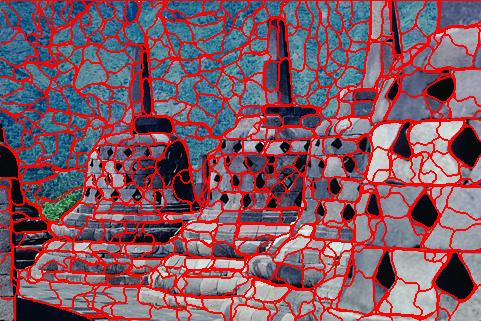
\includegraphics[scale=\scaletwothreebsd]{pictures/bsd-test-1-nc}
	}
	\subfigure{
		\label{subfig:evaluation-qualitative-bsd-2-nc}
		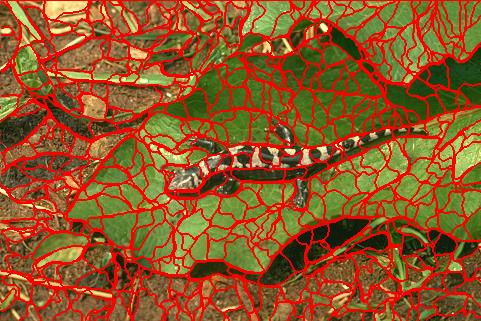
\includegraphics[scale=\scaletwothreebsd]{pictures/bsd-test-2-nc}
	}
	\subfigure{
		\label{subfig:evaluation-qualitative-nyu-1-nc}
		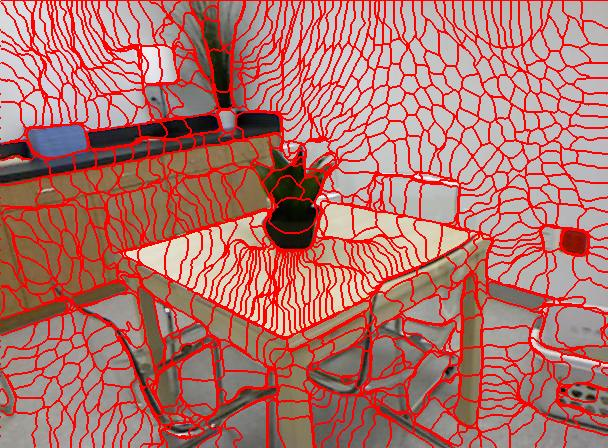
\includegraphics[scale=\scaletwothreenyu]{pictures/nyu-test-1-nc}
	}
	\subfigure{
		\label{subfig:evaluation-qualitative-nyu-2-nc}
		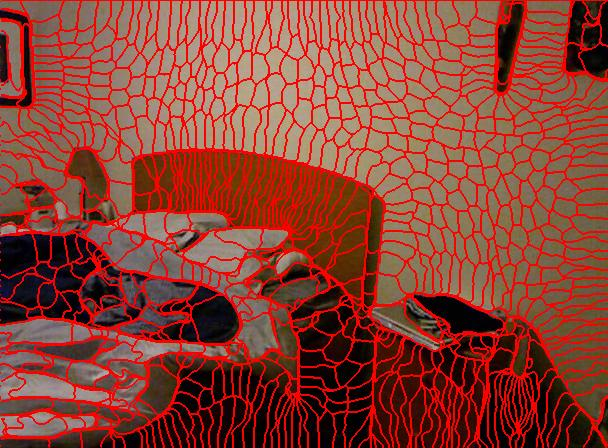
\includegraphics[scale=\scaletwothreenyu]{pictures/nyu-test-2-nc}
	}
	\subfigure{
		\label{subfig:evaluation-qualitative-nyu-3-nc}
		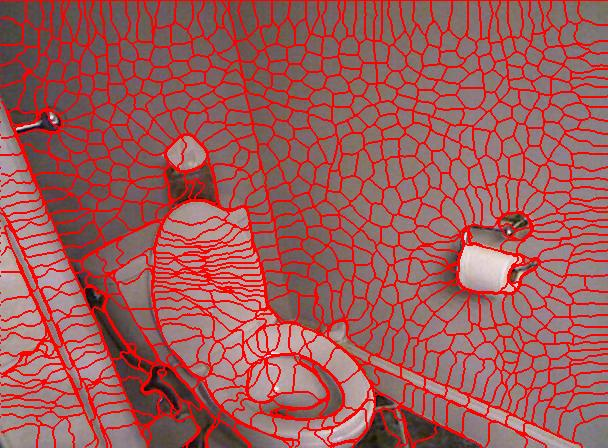
\includegraphics[scale=\scaletwothreenyu]{pictures/nyu-test-3-nc}
	}
	% FH
	\subfigure{
		\label{subfig:evaluation-qualitative-bsd-1-fh}
		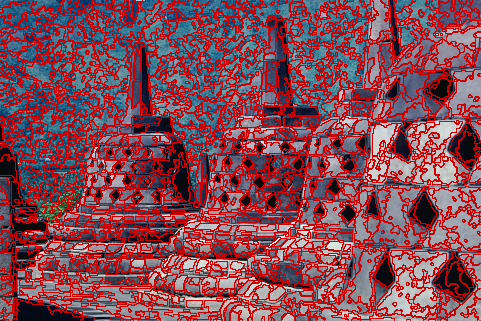
\includegraphics[scale=\scaletwothreebsd]{pictures/bsd-test-1-fh}
	}
	\subfigure{
		\label{subfig:evaluation-qualitative-bsd-2-fh}
		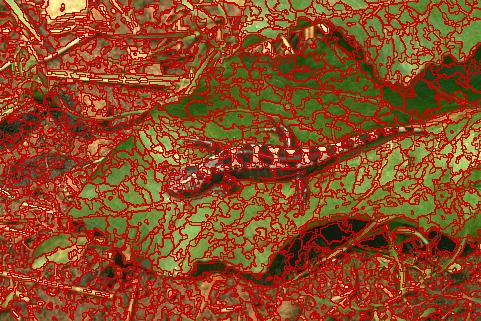
\includegraphics[scale=\scaletwothreebsd]{pictures/bsd-test-2-fh}
	}
	\subfigure{
		\label{subfig:evaluation-qualitative-nyu-1-fh}
		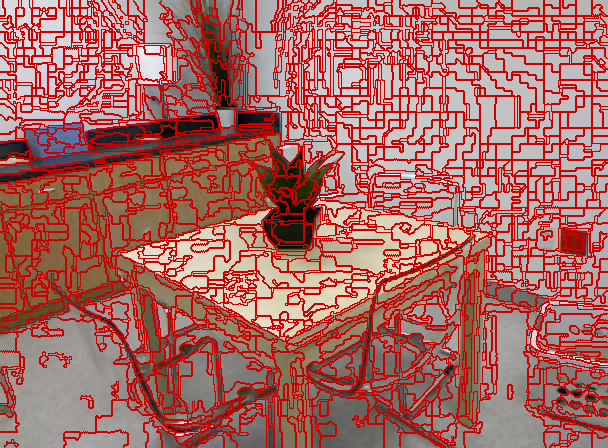
\includegraphics[scale=\scaletwothreenyu]{pictures/nyu-test-1-fh}
	}
	\subfigure{
		\label{subfig:evaluation-qualitative-nyu-2-fh}
		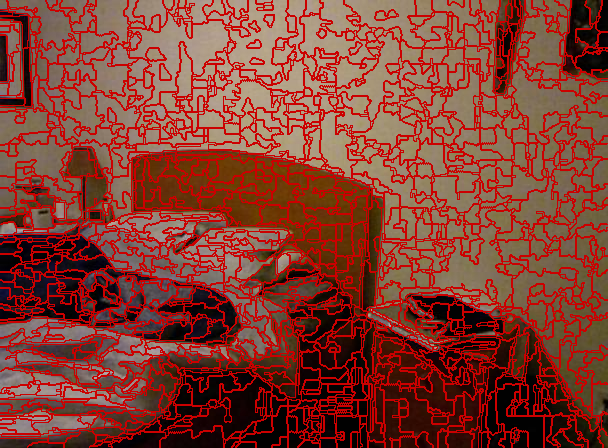
\includegraphics[scale=\scaletwothreenyu]{pictures/nyu-test-2-fh}
	}
	\subfigure{
		\label{subfig:evaluation-qualitative-nyu-3-fh}
		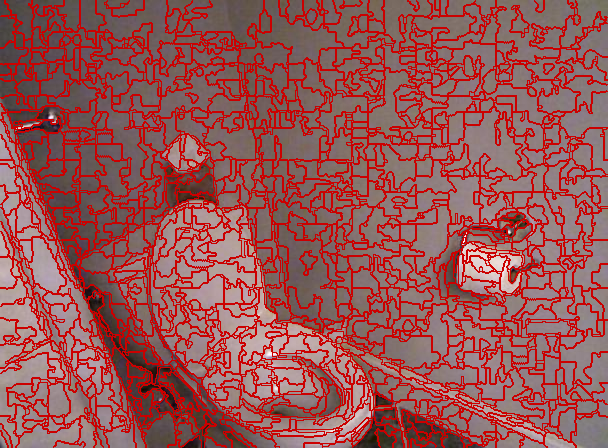
\includegraphics[scale=\scaletwothreenyu]{pictures/nyu-test-3-fh}
	}
	% QS
	\subfigure{
		\label{subfig:evaluation-qualitative-bsd-1-qs}
		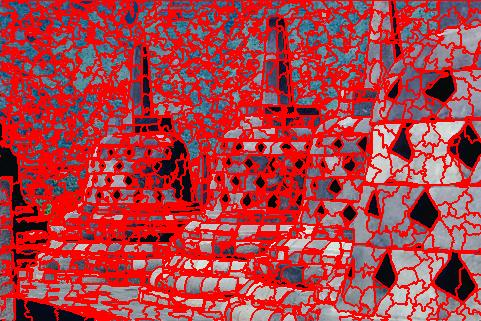
\includegraphics[scale=\scaletwothreebsd]{pictures/bsd-test-1-qs}
	}
	\subfigure{
		\label{subfig:evaluation-qualitative-bsd-2-qs}
		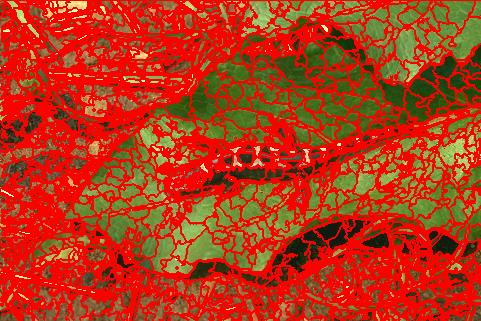
\includegraphics[scale=\scaletwothreebsd]{pictures/bsd-test-2-qs}
	}
	\subfigure{
		\label{subfig:evaluation-qualitative-nyu-1-qs}
		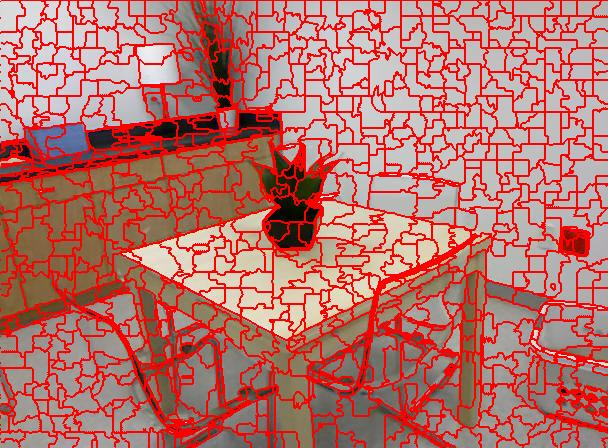
\includegraphics[scale=\scaletwothreenyu]{pictures/nyu-test-1-qs}
	}
	\subfigure{
		\label{subfig:evaluation-qualitative-nyu-2-qs}
		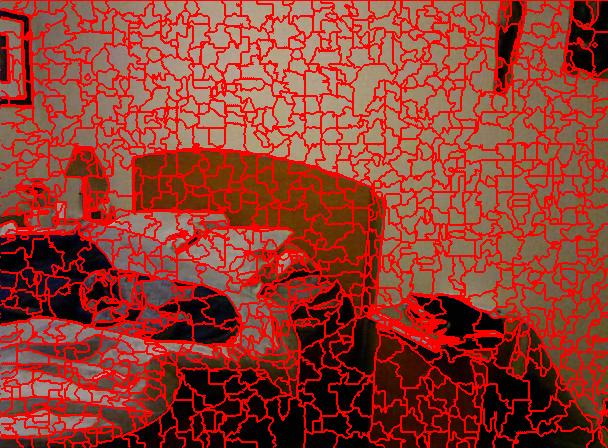
\includegraphics[scale=\scaletwothreenyu]{pictures/nyu-test-2-qs}
	}
	\subfigure{
		\label{subfig:evaluation-qualitative-nyu-3-qs}
		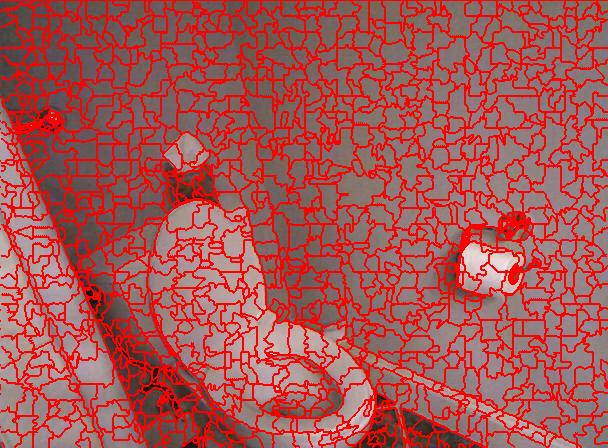
\includegraphics[scale=\scaletwothreenyu]{pictures/nyu-test-3-qs}
	}
	% TP
	\subfigure{
		\label{subfig:evaluation-qualitative-bsd-1-tp}
		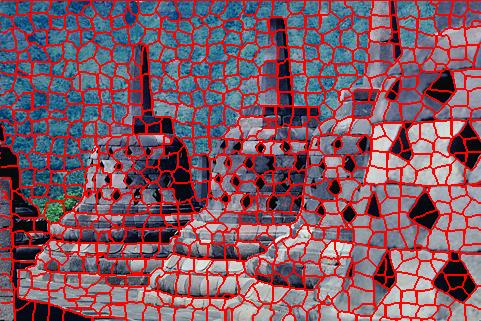
\includegraphics[scale=\scaletwothreebsd]{pictures/bsd-test-1-tp}
	}
	\subfigure{
		\label{subfig:evaluation-qualitative-bsd-2-tp}
		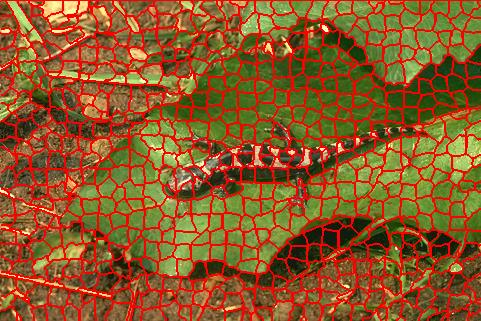
\includegraphics[scale=\scaletwothreebsd]{pictures/bsd-test-2-tp}
	}
	\subfigure{
		\label{subfig:evaluation-qualitative-nyu-1-tp}
		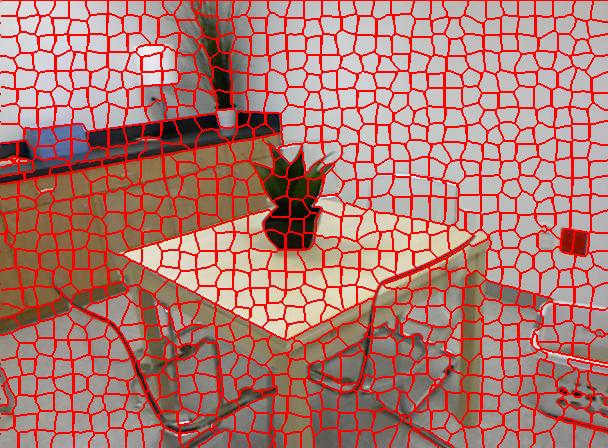
\includegraphics[scale=\scaletwothreenyu]{pictures/nyu-test-1-tp}
	}
	\subfigure{
		\label{subfig:evaluation-qualitative-nyu-2-tp}
		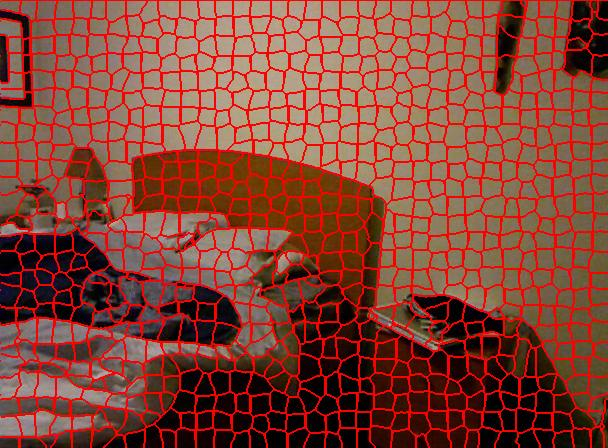
\includegraphics[scale=\scaletwothreenyu]{pictures/nyu-test-2-tp}
	}
	\subfigure{
		\label{subfig:evaluation-qualitative-nyu-3-tp}
		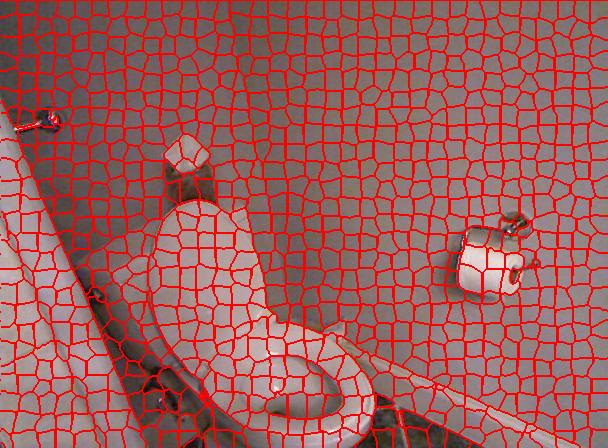
\includegraphics[scale=\scaletwothreenyu]{pictures/nyu-test-3-tp}
	}
	% oriSLIC
	\subfigure{
		\label{subfig:evaluation-qualitative-bsd-1-orislic}
		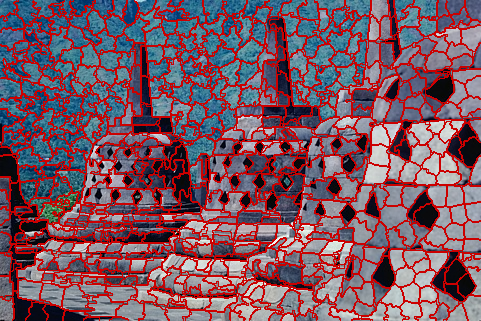
\includegraphics[scale=\scaletwothreebsd]{pictures/bsd-test-1-orislic}
	}
	\subfigure{
		\label{subfig:evaluation-qualitative-bsd-2-orislic}
		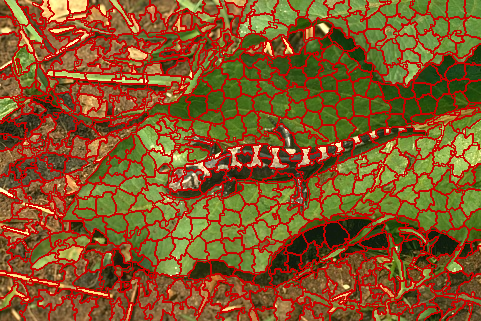
\includegraphics[scale=\scaletwothreebsd]{pictures/bsd-test-2-orislic}
	}
	\subfigure{
		\label{subfig:evaluation-qualitative-nyu-1-orislic}
		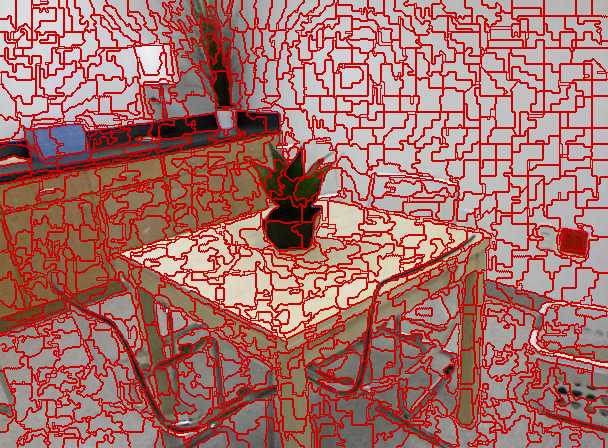
\includegraphics[scale=\scaletwothreenyu]{pictures/nyu-test-1-orislic}
	}
	\subfigure{
		\label{subfig:evaluation-qualitative-nyu-2-orislic}
		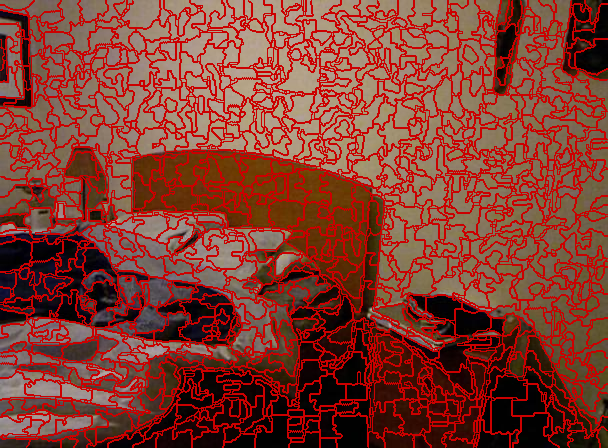
\includegraphics[scale=\scaletwothreenyu]{pictures/nyu-test-2-orislic}
	}
	\subfigure{
		\label{subfig:evaluation-qualitative-nyu-3-orislic}
		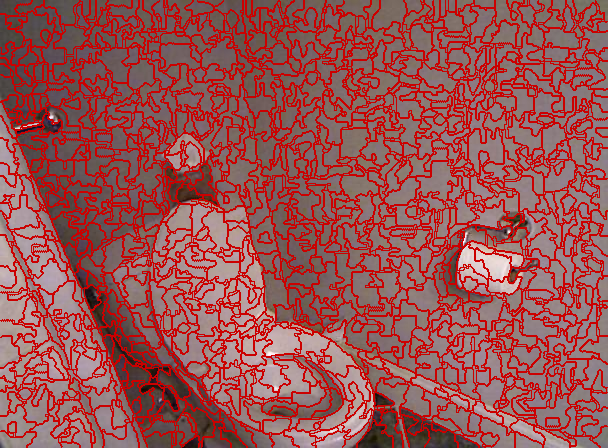
\includegraphics[scale=\scaletwothreenyu]{pictures/nyu-test-3-orislic}
	}
	% CIS
	\subfigure{
		\label{subfig:evaluation-qualitative-bsd-1-cis}
		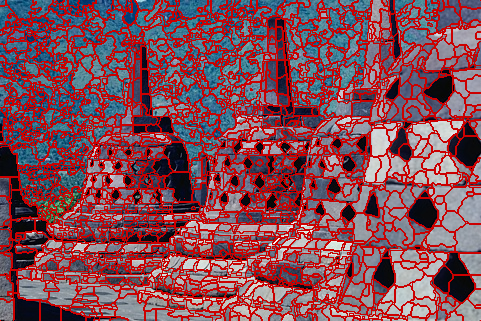
\includegraphics[scale=\scaletwothreebsd]{pictures/bsd-test-1-cis}
	}
	\subfigure{
		\label{subfig:evaluation-qualitative-bsd-2-cis}
		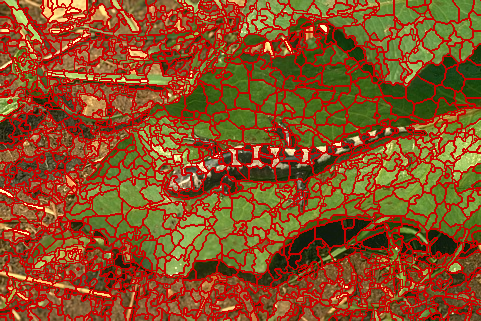
\includegraphics[scale=\scaletwothreebsd]{pictures/bsd-test-2-cis}
	}
	\subfigure{
		\label{subfig:evaluation-qualitative-nyu-1-cis}
		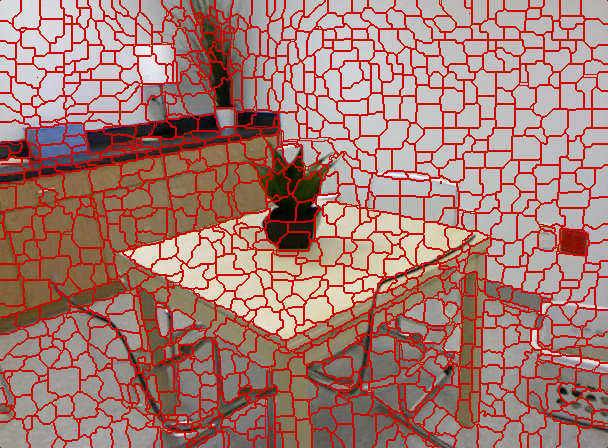
\includegraphics[scale=\scaletwothreenyu]{pictures/nyu-test-1-cis}
	}
	\subfigure{
		\label{subfig:evaluation-qualitative-nyu-2-cis}
		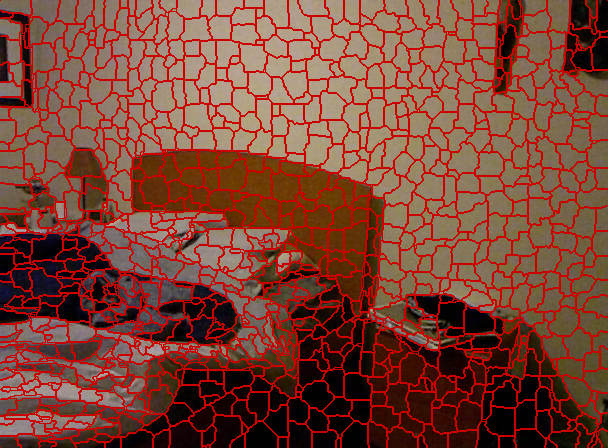
\includegraphics[scale=\scaletwothreenyu]{pictures/nyu-test-2-cis}
	}
	\subfigure{
		\label{subfig:evaluation-qualitative-nyu-3-cis}
		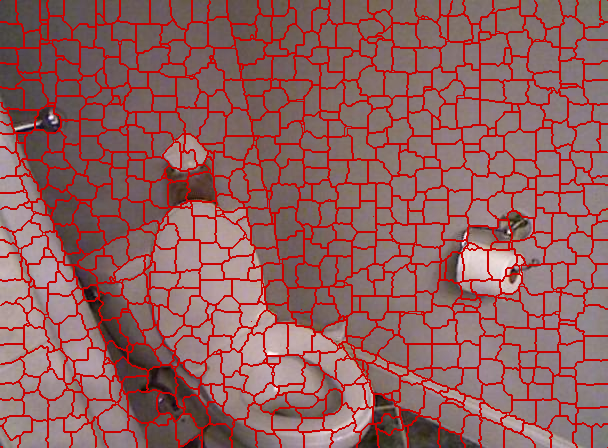
\includegraphics[scale=\scaletwothreenyu]{pictures/nyu-test-3-cis}
	}
	% ERS
	\subfigure{
		\label{subfig:evaluation-qualitative-bsd-1-ers}
		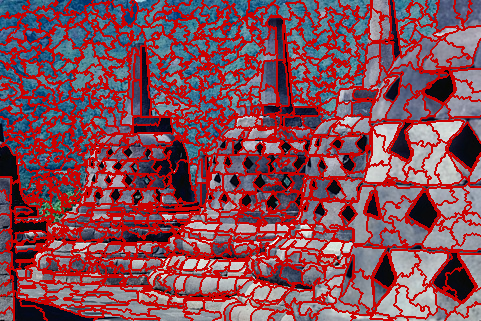
\includegraphics[scale=\scaletwothreebsd]{pictures/bsd-test-1-ers}
	}
	\subfigure{
		\label{subfig:evaluation-qualitative-bsd-2-ers}
		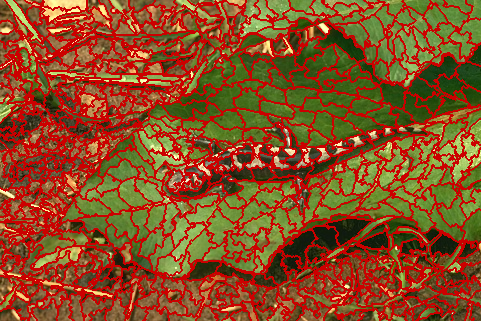
\includegraphics[scale=\scaletwothreebsd]{pictures/bsd-test-2-ers}
	}
	\subfigure{
		\label{subfig:evaluation-qualitative-nyu-1-ers}
		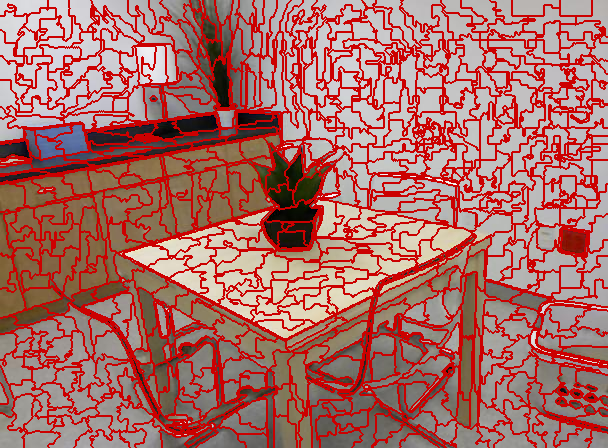
\includegraphics[scale=\scaletwothreenyu]{pictures/nyu-test-1-ers}
	}
	\subfigure{
		\label{subfig:evaluation-qualitative-nyu-2-ers}
		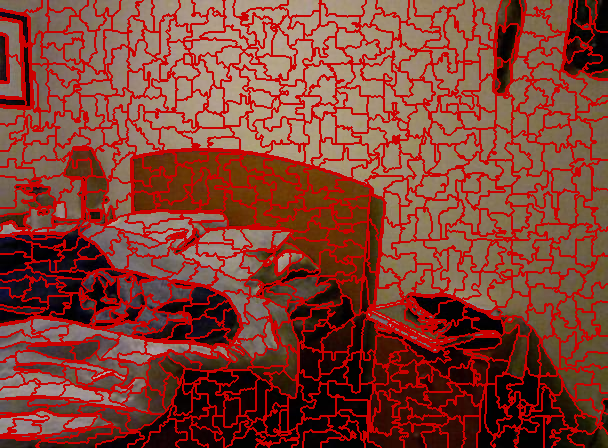
\includegraphics[scale=\scaletwothreenyu]{pictures/nyu-test-2-ers}
	}
	\subfigure{
		\label{subfig:evaluation-qualitative-nyu-3-ers}
		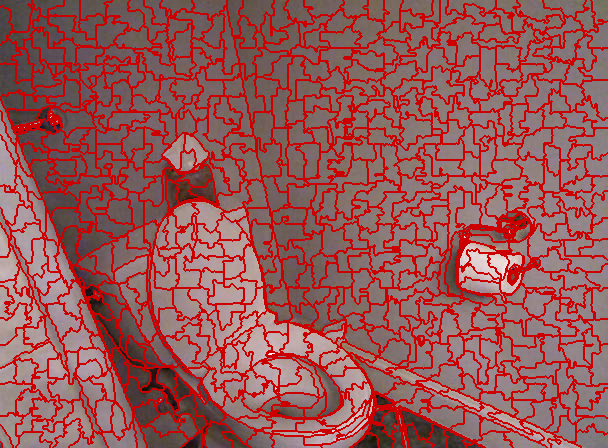
\includegraphics[scale=\scaletwothreenyu]{pictures/nyu-test-3-ers}
	}
	% PB
	\subfigure{
		\label{subfig:evaluation-qualitative-bsd-1-pb}
		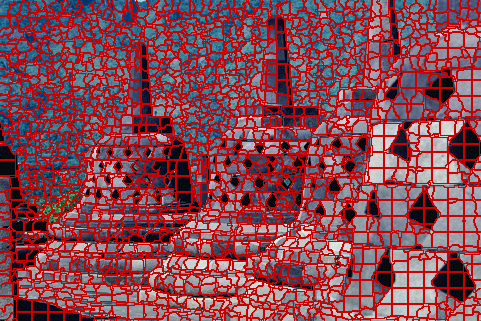
\includegraphics[scale=\scaletwothreebsd]{pictures/bsd-test-1-pb}
	}
	\subfigure{
		\label{subfig:evaluation-qualitative-bsd-2-pb}
		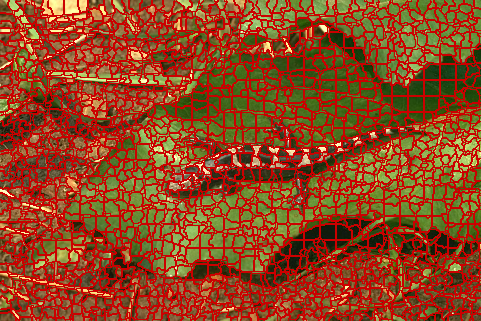
\includegraphics[scale=\scaletwothreebsd]{pictures/bsd-test-2-pb}
	}
	\subfigure{
		\label{subfig:evaluation-qualitative-nyu-1-pb}
		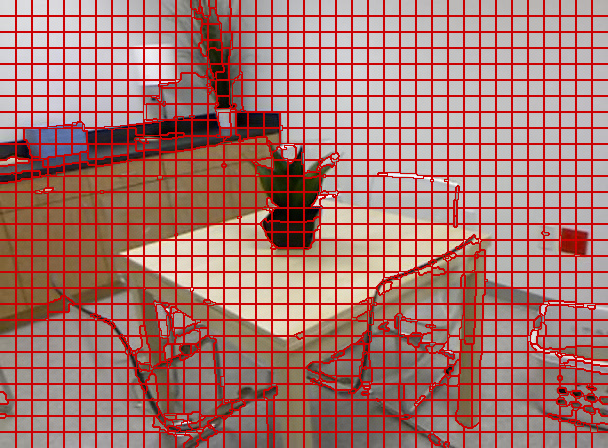
\includegraphics[scale=\scaletwothreenyu]{pictures/nyu-test-1-pb}
	}
	\subfigure{
		\label{subfig:evaluation-qualitative-nyu-2-pb}
		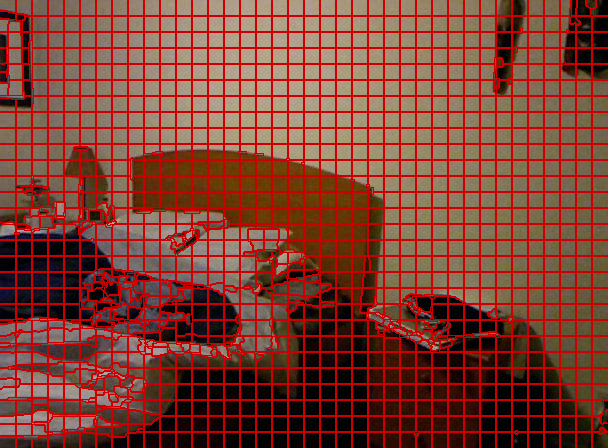
\includegraphics[scale=\scaletwothreenyu]{pictures/nyu-test-2-pb}
	}
	\subfigure{
		\label{subfig:evaluation-qualitative-nyu-3-pb}
		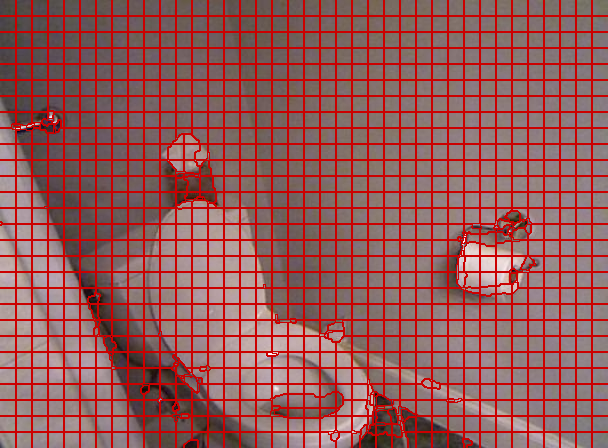
\includegraphics[scale=\scaletwothreenyu]{pictures/nyu-test-3-pb}
	}
	% CRS
	\subfigure{
		\label{subfig:evaluation-qualitative-bsd-1-crs}
		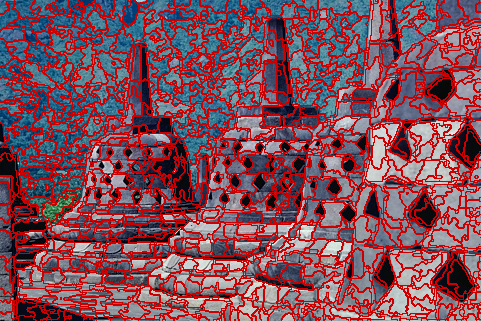
\includegraphics[scale=\scaletwothreebsd]{pictures/bsd-test-1-crs}
	}
	\subfigure{
		\label{subfig:evaluation-qualitative-bsd-2-crs}
		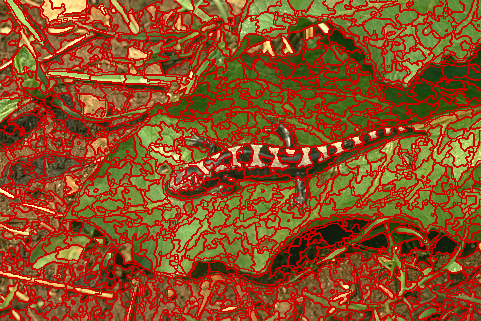
\includegraphics[scale=\scaletwothreebsd]{pictures/bsd-test-2-crs}
	}
	\subfigure{
		\label{subfig:evaluation-qualitative-nyu-1-crs}
		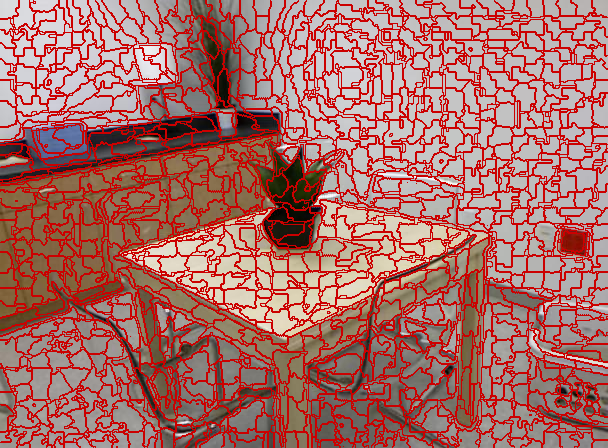
\includegraphics[scale=\scaletwothreenyu]{pictures/nyu-test-1-crs}
	}
	\subfigure{
		\label{subfig:evaluation-qualitative-nyu-2-crs}
		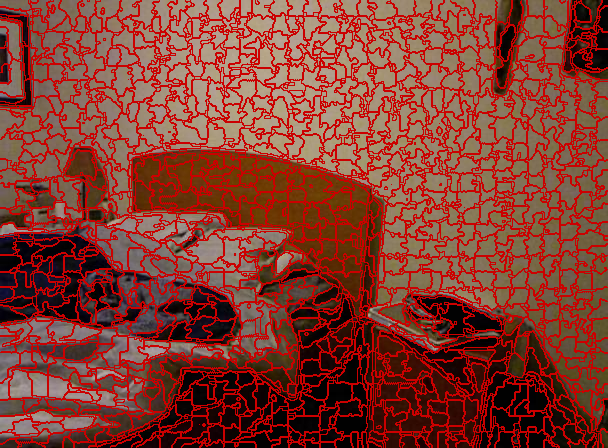
\includegraphics[scale=\scaletwothreenyu]{pictures/nyu-test-2-crs}
	}
	\subfigure{
		\label{subfig:evaluation-qualitative-nyu-3-crs}
		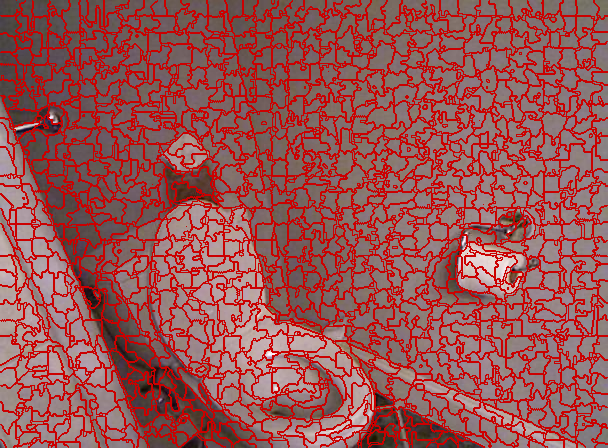
\includegraphics[scale=\scaletwothreenyu]{pictures/nyu-test-3-crs}
	}
	% TPS
	\subfigure{
		\label{subfig:evaluation-qualitative-bsd-1-tps}
		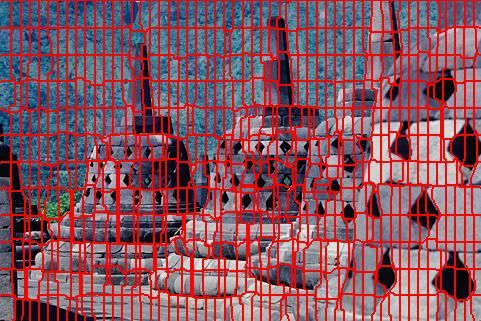
\includegraphics[scale=\scaletwothreebsd]{pictures/bsd-test-1-tps}
	}
	\subfigure{
		\label{subfig:evaluation-qualitative-bsd-2-tps}
		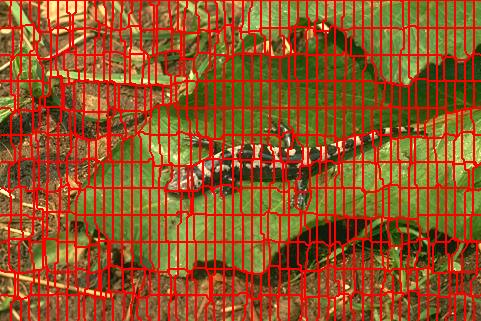
\includegraphics[scale=\scaletwothreebsd]{pictures/bsd-test-2-tps}
	}
	\subfigure{
		\label{subfig:evaluation-qualitative-nyu-1-tps}
		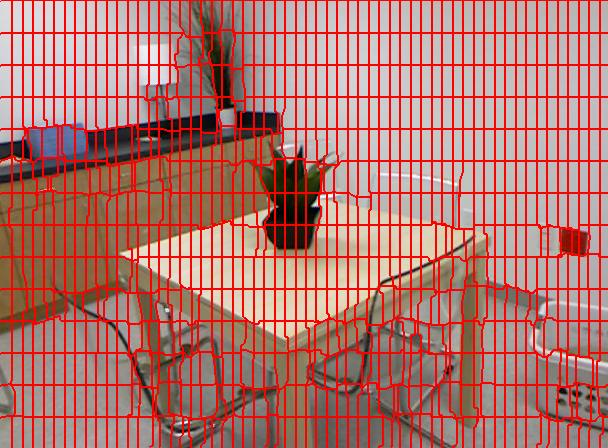
\includegraphics[scale=\scaletwothreenyu]{pictures/nyu-test-1-tps}
	}
	\subfigure{
		\label{subfig:evaluation-qualitative-nyu-2-tps}
		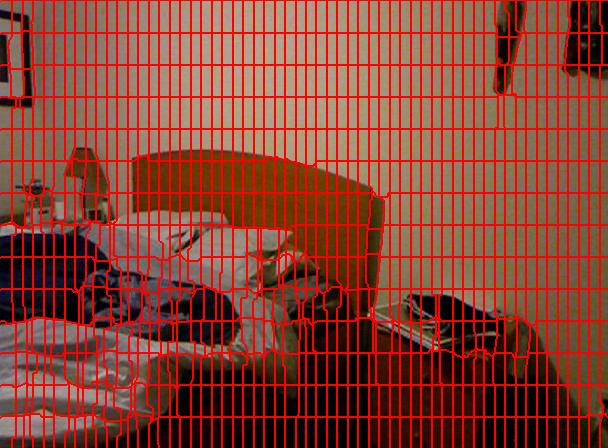
\includegraphics[scale=\scaletwothreenyu]{pictures/nyu-test-2-tps}
	}
	\subfigure{
		\label{subfig:evaluation-qualitative-nyu-3-tps}
		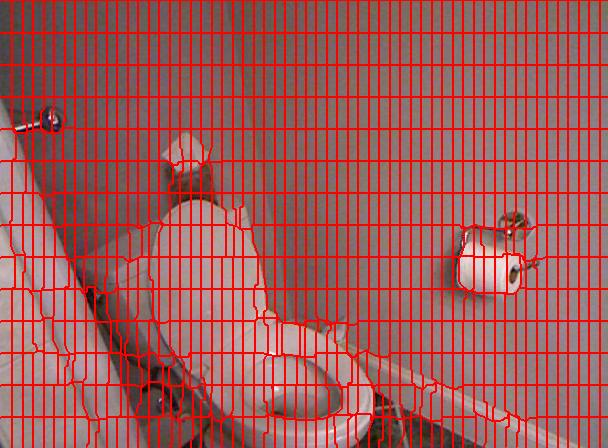
\includegraphics[scale=\scaletwothreenyu]{pictures/nyu-test-3-tps}
	}
	% TODO: add vlSLIC if applicable.
	\caption[Qualitative results for \textbf{NC} \cite{RenMalik:2003}, \textbf{FH} \cite{FelzenswalbHuttenlocher:2004}, \textbf{QS} \cite{VedaldiSoatto:2008}, \textbf{TP} \cite{LevinshteinStereKutulakosFleetDickinsonSiddiqi:2009}, \textbf{SLIC} \cite{AchantaShajiSmithLucchiFuaSuesstrunk:2010}, \textbf{CIS} \cite{VekslerBoykovMehrani:2010}, \textbf{ERS} \cite{LiuTuzelRamalingamChellappa:2011}, \textbf{PB} \cite{ZhangHartleyMashfordBurn:2011}, \textbf{CRS} \cite{ConradMertzMester:2013} and \textbf{TPS} \cite{DaiTangHuazhaFuXiaochunCao:2012} illustrated on images from the Berkeley Segmentation Dataset \cite{ArbelaezMaireFowlkesMalik:2011} and the NYU Depth Dataset \cite{SilbermanHoiemKohliFergus:2012}.]{Qualitative results for several evaluated superpixel algorithms illustrated on two images form the BSDS500 and three images from the NYUV2. From top to bottom: \textbf{NC}, \textbf{FH}, \textbf{QS}, \textbf{TP}, \textbf{oriSLIC}, \textbf{CIS}, \textbf{ERS}, \textbf{PB}, \textbf{CRS}, \textbf{TPS}. For images from the BSDS500, approximately $600$ superpixels are shown; for images from the NYUV2 approximately $840$ images are shown. Further examples can be found in appendix \ref{chapter:appendix-evaluation}.}
	\label{fig:evaluation-qualitative}
\end{figure}

\textbf{NC}. Superpixels from Normalized Cuts are relatively smooth when compared to other approaches, however, tend to be highly elongated in order to adhere to boundaries. Mostly, strong boundaries are met well, but smaller objects and details are missed.

\textbf{FH}. Superpixels generated by \textbf{FH} cannot be described as regular or compact. However, they are able to adapt even to small details. This leads to a good overall boundary adherence. In addition, we often observe collapsed superpixels within relatively large superpixels.

\textbf{QS}. Similar to \textbf{FH}, \textbf{QS} generates superpixels irregular in size and shape. However, superpixels are able to capture little details. Furthermore, we notice that the number of superpixels adapts to the image content in that more superpixels are found at strongly textured regions.% However, at nearly uniformly colored regions the superpixels show irregular behavior.
\begin{figure}[t]
	\centering
	% oriSEEDS
	\subfigure{
		\label{subfig:evaluation-qualitative-bsd-1-oriseeds}
		\includegraphics[scale=\scaletwothreebsd]{pictures/bsd-test-1-oriseeds}
	}
	\subfigure{
		\label{subfig:evaluation-qualitative-bsd-2-oriseeds}
		\includegraphics[scale=\scaletwothreebsd]{pictures/bsd-test-2-oriseeds}
	}
	\subfigure{
		\label{subfig:evaluation-qualitative-nyu-1-oriseeds}
		\includegraphics[scale=\scaletwothreenyu]{pictures/nyu-test-1-oriseeds}
	}
	\subfigure{
		\label{subfig:evaluation-qualitative-nyu-2-oriseeds}
		\includegraphics[scale=\scaletwothreenyu]{pictures/nyu-test-2-oriseeds}
	}
	\subfigure{
		\label{subfig:evaluation-qualitative-nyu-3-oriseeds}
		\includegraphics[scale=\scaletwothreenyu]{pictures/nyu-test-3-oriseeds}
	}
	% oriSEEDSmp
	\subfigure{
		\label{subfig:evaluation-qualitative-bsd-1-oriseedsmp}
		\includegraphics[scale=\scaletwothreebsd]{pictures/bsd-test-1-oriseedsmp}
	}
	\subfigure{
		\label{subfig:evaluation-qualitative-bsd-2-oriseedsmp}
		\includegraphics[scale=\scaletwothreebsd]{pictures/bsd-test-2-oriseedsmp}
	}
	\subfigure{
		\label{subfig:evaluation-qualitative-nyu-1-oriseedsmp}
		\includegraphics[scale=\scaletwothreenyu]{pictures/nyu-test-1-oriseedsmp}
	}
	\subfigure{
		\label{subfig:evaluation-qualitative-nyu-2-oriseedsmp}
		\includegraphics[scale=\scaletwothreenyu]{pictures/nyu-test-2-oriseedsmp}
	}
	\subfigure{
		\label{subfig:evaluation-qualitative-nyu-3-oriseedsmp}
		\includegraphics[scale=\scaletwothreenyu]{pictures/nyu-test-3-oriseedsmp}
	}
	% reSEEDS
	\subfigure{
		\label{subfig:evaluation-qualitative-bsd-1-reseeds}
		\includegraphics[scale=\scaletwothreebsd]{pictures/bsd-test-1-reseeds}
	}
	\subfigure{
		\label{subfig:evaluation-qualitative-bsd-2-reseeds}
		\includegraphics[scale=\scaletwothreebsd]{pictures/bsd-test-2-reseeds}
	}
	\subfigure{
		\label{subfig:evaluation-qualitative-nyu-1-reseeds}
		\includegraphics[scale=\scaletwothreenyu]{pictures/nyu-test-1-reseeds}
	}
	\subfigure{
		\label{subfig:evaluation-qualitative-nyu-2-reseeds}
		\includegraphics[scale=\scaletwothreenyu]{pictures/nyu-test-2-reseeds}
	}
	\subfigure{
		\label{subfig:evaluation-qualitative-nyu-3-reseeds}
		\includegraphics[scale=\scaletwothreenyu]{pictures/nyu-test-3-reseeds}
	}
	% reSEEDSmp
	\subfigure{
		\label{subfig:evaluation-qualitative-bsd-1-reseedsmp}
		\includegraphics[scale=\scaletwothreebsd]{pictures/bsd-test-1-reseedsmp}
	}
	\subfigure{
		\label{subfig:evaluation-qualitative-bsd-2-reseedsmp}
		\includegraphics[scale=\scaletwothreebsd]{pictures/bsd-test-2-reseedsmp}
	}
	\subfigure{
		\label{subfig:evaluation-qualitative-nyu-1-reseedsmp}
		\includegraphics[scale=\scaletwothreenyu]{pictures/nyu-test-1-reseedsmp}
	}
	\subfigure{
		\label{subfig:evaluation-qualitative-nyu-2-reseedsmp}
		\includegraphics[scale=\scaletwothreenyu]{pictures/nyu-test-2-reseedsmp}
	}
	\subfigure{
		\label{subfig:evaluation-qualitative-nyu-3-reseedsmp}
		\includegraphics[scale=\scaletwothreenyu]{pictures/nyu-test-3-reseedsmp}
	}
	% reSEEDSmp*
	\subfigure{
		\label{subfig:evaluation-qualitative-bsd-1-reseedssm}
		\includegraphics[scale=\scaletwothreebsd]{pictures/bsd-test-1-reseedssm}
	}
	\subfigure{
		\label{subfig:evaluation-qualitative-bsd-2-reseedssm}
		\includegraphics[scale=\scaletwothreebsd]{pictures/bsd-test-2-reseedssm}
	}
	\subfigure{
		\label{subfig:evaluation-qualitative-nyu-1-reseedssm}
		\includegraphics[scale=\scaletwothreenyu]{pictures/nyu-test-1-reseedssm}
	}
	\subfigure{
		\label{subfig:evaluation-qualitative-nyu-2-reseedssm}
		\includegraphics[scale=\scaletwothreenyu]{pictures/nyu-test-2-reseedssm}
	}
	\subfigure{
		\label{subfig:evaluation-qualitative-nyu-3-reseedssm}
		\includegraphics[scale=\scaletwothreenyu]{pictures/nyu-test-3-reseedssm}
	}
	\caption[Qualitative results for all implementations of \textbf{SEEDS} \cite{VanDenBerghBoixRoigCapitaniVanGool:2012} on images from the Berkeley Segmentation Dataset \cite{ArbelaezMaireFowlkesMalik:2011} and the NYU Depth Dataset \cite{SilbermanHoiemKohliFergus:2012}.]{Qualitative results for all implementations of \textbf{SEEDS} illustrated on two images form the BSDS500 and three images from the NYUV2. From top to bottom: \textbf{oriSEEDS}, \textbf{oriSEEDSmp}, \textbf{reSEEDS}, \textbf{reSEEDSmp}, \textbf{reSEEDSmp*}. For images from the BSDS500, approximately $600$ superpixels are shown; for images from the NYUV2 approximately $840$ images are shown. Further examples can be found in appendix \ref{chapter:appendix-evaluation}.}
	\label{fig:evaluation-qualitative-seeds}
\end{figure}

\textbf{TP}. A strong focus on compactness often results in poor boundary adherence. This can be observed when considering superpixels generated by \textbf{TP}. In particular, objects or details smaller than the initial regular grid are rarely captured well. However, when increasing the number of superpixels, boundary adherence may be combined with very compact superpixels.

\textbf{SLIC} is one of the few algorithms offering direct control over the compactness. Therefore, using \textbf{SLIC} may result in visually appealing, regular and compact superpixels. However, the compactness needs to be traded off against Boundary Recall and Undersegmentation Error. As we optimized the parameters with respect to Boundary Recall and Undersegmentation Error, we get relatively irregular superpixels at nearly uniformly colored regions but on the other hand are able to capture small details. This gets apparent on images from the NYUV2.

\textbf{SLIC3D}. Superpixels generated by \textbf{SLIC3D} are similar to those generated by \textbf{SLIC}. On some images, the superpixels appear relatively compact on nearly uniformly colored regions while on others we can observe highly irregular superpixels. Overall, the superpixels are able to adapt to comparably small details and lighting changes.

\textbf{CIS}. As \textbf{CIS} uses gray scale images only, some boundaries are inevitable missed. Additionally, \textbf{CIS} gets easily challenged by small details as well as bad lighting. However, the superpixels appear to be relatively compact and regular when compared to other approaches not offering direct control over the compactness. Some of these disadvantages may be resolved when extending \textbf{CIS} to use color images.

\textbf{ERS}. Superpixels generated by \textbf{ERS} show a good boundary adherence. This is partly due to the large variation in size: \textbf{ERS} superpixels are able to adapt their size to capture small details. At nearly uniformly colored regions, the superpixels tend to be irregular and are not visually appealing anymore.

\textbf{PB}. Superpixels generated by \textbf{PB} appear to be unfinished and of poor quality. Often, the superpixels tend to be too regular and compact such that even strong boundaries are not captured well. In particular, this can be observed for images taken from the NYUV2. Even strong changes in color do not affect the initial superpixel segmentation given by a regular grid.

\textbf{CRS}. Similar to \textbf{SLIC}, \textbf{CRS} offers direct control over the compactness. As we optimized the parameters with respect to Boundary Recall and Undersegmentation Error, the generated superpixels do not appear compact, especially on images from the NYUV2. However, this enables superpixels to capture small details and achieve reasonable boundary adherence. Increasing the number of superpixels as well as the compactness parameter will result in visually more appealing superpixels with similar performance.

\begin{figure}[t]
	\centering
	% SLIC3D
	\subfigure{
		\label{subfig:evaluation-qualitative-nyu-1-slic3d-beta-10}
		\includegraphics[scale=\scaletwothreenyu]{pictures/nyu-test-1-slic3d}
	}
	\subfigure{
		\label{subfig:evaluation-qualitative-nyu-2-slic3d-beta-10}
		\includegraphics[scale=\scaletwothreenyu]{pictures/nyu-test-2-slic3d}
	}
	\subfigure{
		\label{subfig:evaluation-qualitative-nyu-3-slic3d-beta-10}
		\includegraphics[scale=\scaletwothreenyu]{pictures/nyu-test-3-slic3d}
	}
	\subfigure{
		\label{subfig:evaluation-qualitative-nyu-4-slic3d-beta-10}
		\includegraphics[scale=\scaletwothreenyu]{pictures/nyu-test-4-slic3d}
	}
	\subfigure{
		\label{subfig:evaluation-qualitative-nyu-5-slic3d-beta-10}
		\includegraphics[scale=\scaletwothreenyu]{pictures/nyu-test-5-slic3d}
	}
	% SEEDS3D
	\subfigure{
		\label{subfig:evaluation-qualitative-nyu-1-seeds3d}
		\includegraphics[scale=\scaletwothreenyu]{pictures/nyu-test-1-seeds3d}
	}
	\subfigure{
		\label{subfig:evaluation-qualitative-nyu-2-seeds3d}
		\includegraphics[scale=\scaletwothreenyu]{pictures/nyu-test-2-seeds3d}
	}
	\subfigure{
		\label{subfig:evaluation-qualitative-nyu-3-seeds3d}
		\includegraphics[scale=\scaletwothreenyu]{pictures/nyu-test-3-seeds3d}
	}
	\subfigure{
		\label{subfig:evaluation-qualitative-nyu-4-seeds3d}
		\includegraphics[scale=\scaletwothreenyu]{pictures/nyu-test-4-seeds3d}
	}
	\subfigure{
		\label{subfig:evaluation-qualitative-nyu-5-seeds3d}
		\includegraphics[scale=\scaletwothreenyu]{pictures/nyu-test-5-seeds3d}
	}
	% SEEDS3Dn
	\subfigure{
		\label{subfig:evaluation-qualitative-nyu-1-seeds3dn}
		\includegraphics[scale=\scaletwothreenyu]{pictures/nyu-test-1-seeds3dn}
	}
	\subfigure{
		\label{subfig:evaluation-qualitative-nyu-2-seeds3dn}
		\includegraphics[scale=\scaletwothreenyu]{pictures/nyu-test-2-seeds3dn}
	}
	\subfigure{
		\label{subfig:evaluation-qualitative-nyu-3-seeds3dn}
		\includegraphics[scale=\scaletwothreenyu]{pictures/nyu-test-3-seeds3dn}
	}
	\subfigure{
		\label{subfig:evaluation-qualitative-nyu-4-seeds3dn}
		\includegraphics[scale=\scaletwothreenyu]{pictures/nyu-test-4-seeds3dn}
	}
	\subfigure{
		\label{subfig:evaluation-qualitative-nyu-5-seeds3dn}
		\includegraphics[scale=\scaletwothreenyu]{pictures/nyu-test-5-seeds3dn}
	}
	% DASP
	\subfigure{
		\label{subfig:evaluation-qualitative-nyu-1-dasp}
		\includegraphics[scale=\scaletwothreenyu]{{pictures/nyu-test-1-dasp-beta-0.05}.png}
	}
	\subfigure{
		\label{subfig:evaluation-qualitative-nyu-2-dasp}
		\includegraphics[scale=\scaletwothreenyu]{{pictures/nyu-test-2-dasp-beta-0.05}.png}
	}
	\subfigure{
		\label{subfig:evaluation-qualitative-nyu-3-dasp}
		\includegraphics[scale=\scaletwothreenyu]{{pictures/nyu-test-3-dasp-beta-0.05}.png}
	}
	\subfigure{
		\label{subfig:evaluation-qualitative-nyu-4-dasp}
		\includegraphics[scale=\scaletwothreenyu]{{pictures/nyu-test-4-dasp-beta-0.05}.png}
	}
	\subfigure{
		\label{subfig:evaluation-qualitative-nyu-5-dasp}
		\includegraphics[scale=\scaletwothreenyu]{{pictures/nyu-test-5-dasp-beta-0.05}.png}
	}
	% DCRS
	% VCCS
	\subfigure{
		\label{subfig:evaluation-qualitative-nyu-1-vccs}
		\includegraphics[scale=\scaletwothreenyu]{pictures/nyu-test-1-vccs}
	}
	\subfigure{
		\label{subfig:evaluation-qualitative-nyu-2-vccs}
		\includegraphics[scale=\scaletwothreenyu]{pictures/nyu-test-2-vccs}
	}
	\subfigure{
		\label{subfig:evaluation-qualitative-nyu-3-vccs}
		\includegraphics[scale=\scaletwothreenyu]{pictures/nyu-test-3-vccs}
	}
	\subfigure{
		\label{subfig:evaluation-qualitative-nyu-4-vccs}
		\includegraphics[scale=\scaletwothreenyu]{pictures/nyu-test-4-vccs}
	}
	\subfigure{
		\label{subfig:evaluation-qualitative-nyu-5-vccs}
		\includegraphics[scale=\scaletwothreenyu]{pictures/nyu-test-5-vccs}
	}
	\caption[Qualitative results for an extension of \textbf{SEEDS} \cite{VanDenBerghBoixRoigCapitaniVanGool:2012} using depth information, \textbf{DASP} \cite{WeikersdorferGossowBeetz:2012} and \textbf{VCCS} \cite{PaponAbramovSchoelerWoergoetter:2013} on images from the NYU Depth Dataset \cite{SilbermanHoiemKohliFergus:2012}.]{Qualitative results for superpixel algorithms utilizing depth. From top to bottom: \textbf{SLIC3D}, \textbf{SEEDS3D}, \textbf{SEEDS3Dn}, \textbf{DASP}, \textbf{VCCS}. For images from the BSDS500, approximately $600$ superpixels are shown; for images from the NYUV2 approximately $840$ images are shown. Further examples can be found in appendix \ref{chapter:appendix-evaluation}.}
	\label{fig:evaluation-qualitative-depth}
\end{figure}
\textbf{SEEDS}. Independent of the implementation, using \textbf{SEEDS} without mean pixel updates (that is \textbf{oriSEEDS} and \textbf{reSEEDS} for the original and our implementation, respectively) results in highly irregular superpixels which are mostly not compact. However, especially on images from the BSDS500, the superpixel segmentations show good boundary adherence. On images from the NYUV2, the original implementation shows poor boundary adherence compared to our implementation. Using mean pixel updates (that is \textbf{oriSEEDSmp} and \textbf{reSEEDSmp} for the original and or implementation, respectively) results in improved boundary adherence. The superpixels are able to capture small details at the cost of regularity and compactness. At this point, using the alternative smoothing term of equation \eqref{eq:superpixel-segmentation-seeds-spatial-smoothing}, referred to as \textbf{reSEEDSmp*}, generates more compact as well as regular superpixels. Nevertheless, these superpixels are able to adapt to small details and boundaries. 

\textbf{SEEDS3D}. Superpixels generated by \textbf{SEEDS3D} appear to be similar to those obtained from \textbf{reSEEDSmp*}. However, the superpixels appear to resemble the underlying three dimensional structure better. Additionally, the superpixels are adaptive to small changes in color as well as lighting changes. Unfortunately, we observe collapsed superpixels especially at nearly uniformly colored regions. \textbf{SEEDS3Dn} appears to worsen the results, at least concerning the visual quality of the superpixels. As of the negligible performance improvement of \textbf{SEEDS3Dn} over \textbf{SEEDS3D}, we further concentrate on \textbf{SEEDS3D}.

\textbf{DASP}. Superpixels generated by \textbf{DASP} are overall not visually appealing. However, note that \textbf{DASP} allows to adjust the compactness of the superpixels. In addition, the algorithm is not robust to noise within the depth image. This can be observed at regions where depth has been filled, especially towards the borders. Often strong boundaries are not captured well, although the superpixels are allowed to vary in size and shape.

\textbf{TPS}. Superpixels generated by \textbf{TPS} should resemble a regular topology. However, often the superpixel segmentation appears to be of poor quality as we are able to think of better topology preserving superpixel segmentations \cite{DaiTangHuazhaFuXiaochunCao:2012} adhering to more of the strong boundaries present in the images. On images from the NYUV2 this may be due to the fact that the underlying contour detector \cite{ArbelaezMaireFowlkesMalik:2011} has been trained on the BSDS500, however, even on images from the BSDS500 the quality is relatively poor.

\textbf{VCCS}. As \textbf{VCCS} is designed to work directly on point clouds, the generated supervoxels can best be observed on the oversegmented point clouds. Figure \ref{fig:evaluation-qualitative-depth} merely shows the backprojection of the oversegmented point cloud. This means, that the effect of voxelization is still visible. As we chose to optimize Boundary Recall and Undersegmentation Error, the supervoxels are irregular and not compact. However, this can be controlled by the provided compactness parameter. The supervoxels align well with most of the visible boundaries, and are able to capture small details.

% ============================================================
% quantitative \/
\subsection{Quantitative}

The quantitative evaluation is based on the measures provided in section \ref{section:datasets-extended-berkeley-segmentation-benchmark}. Although Boundary Recall and Undersegmentation Error may give a good idea of the performance of an algorithm, additional measures are necessary to complement the impression. Therefore, we use Achievable Segmentation Accuracy, Compactness, Sum-of-Squared Error as well as Explained Variation. We note that due to the prohibitive runtime of \textbf{NC}, the results obtained on the smaller validation set of the BSDS500 and training set of NYUV2 are used. Unfortunately, we were not able to evaluate \textbf{CIS} and \textbf{TPS} with respect to the Sum-of-Squared Error and Explained Variation. All results are also available in tabular form in appendix \ref{chapter:appendix-evaluation}.

\begin{figure}[t]
	\centering
	\subfigure{
		\begin{tikzpicture}
			\begin{axis}[
					height=6.4cm,
					width=3.75cm,
					xlabel=Superpixels,
					ylabel=$Rec$,
					ymin=0.9,
					ymax=1,
					xmin=100,
					xmax=1200,
					cycle list name=comparison bsd]
					
				% NC
				\addplot+[thick] table [row sep=newline,trim cells=true,x=K,y=Rec] {data/nc-bsd.csv};
				\label{plot:evaluation-comparison-nc-rec-bsd}
				
				% FH
				\addplot+[thick] table [row sep=newline,trim cells=true,x=K,y=Rec] {data/fh-bsd-test.csv};
				\label{plot:evaluation-comparison-fh-rec-bsd}
				
				% QS
				\addplot+[thick] table [row sep=newline,trim cells=true,x=K,y=Rec] {data/qs-bsd-test.csv};
				\label{plot:evaluation-comparison-qs-rec-bsd}
				
				% TP
				\addplot+[thick] table [row sep=newline,trim cells=true,x=K,y=Rec] {data/tp-bsd-test.csv};
				\label{plot:evaluation-comparison-tp-rec-bsd}
				
				% oriSLIC
				\addplot+[thick] table [row sep=newline,trim cells=true,x=K,y=Rec] {data/orislic-bsd-test.csv};
				\label{plot:evaluation-comparison-orislic-rec-bsd}
				
				% CIS
				\addplot+[thick] table [row sep=newline,trim cells=true,x=K,y=Rec] {data/cis-bsd-test.csv};
				\label{plot:evaluation-comparison-cis-rec-bsd}
				
				% ERS
				\addplot+[thick] table [row sep=newline,trim cells=true,x=K,y=Rec] {data/ers-bsd-test.csv};
				\label{plot:evaluation-comparison-ers-rec-bsd}
				
				% PB
				\addplot+[thick] table [row sep=newline,trim cells=true,x=K,y=Rec] {data/pb-bsd-test.csv};
				\label{plot:evaluation-comparison-pb-rec-bsd}
				
				% oriSEEDSmp
				\addplot+[thick] table [row sep=newline,trim cells=true,x=K,y=Rec] {data/oriseedsmp-bsd-test.csv};
				\label{plot:evaluation-comparison-oriseedsmp-rec-bsd}
				
				% reSEEDSmp*
				\addplot+[thick] table [row sep=newline,trim cells=true,x=K,y=Rec] {data/reseedssm-bsd-test.csv};
				\label{plot:evaluation-comparison-reseedssm-rec-bsd}
				
				% TPS
				\addplot+[thick] table [row sep=newline,trim cells=true,x=K,y=Rec] {data/tps-bsd-test.csv};
				\label{plot:evaluation-comparison-tps-rec-bsd}
				
				% CRS
				\addplot+[thick] table [row sep=newline,trim cells=true,x=K,y=Rec] {data/crs-bsd-test.csv};
				\label{plot:evaluation-comparison-crs-rec-bsd}
			\end{axis}
%			\matrix[%
%					matrix of nodes,%
%					anchor=north west,%
%					inner sep=0.15em,%
%					nodes={font=\scriptsize},%
%					column 1/.append style={anchor=base west},%
%				] at ($(current axis.north east) + (0.25,0)$) {
%					BSDS500:\\
%					\ref{plot:evaluation-comparison-nc-rec-bsd} \textbf{NC}
%					\ref{plot:evaluation-comparison-qs-rec-bsd} \textbf{FH}\\
%					\ref{plot:evaluation-comparison-fh-rec-bsd} \textbf{QS}
%					\ref{plot:evaluation-comparison-tp-rec-bsd} \textbf{TP}\\
%					\ref{plot:evaluation-comparison-orislic-rec-bsd} \textbf{oriSLIC}\\
%					% vlSLIC
%					\ref{plot:evaluation-comparison-cis-rec-bsd} \textbf{CIS}
%					\ref{plot:evaluation-comparison-ers-rec-bsd} \textbf{ERS}\\
%					\ref{plot:evaluation-comparison-pb-rec-bsd} \textbf{PB}\\
%					\ref{plot:evaluation-comparison-oriseedsmp-rec-bsd} \textbf{oriSEEDSmp}\\
%					\ref{plot:evaluation-comparison-reseedssm-rec-bsd} \textbf{reSEEDSmp*}\\
%					% \ref{plot:evaluation-comparison-tps-rec-bsd} \textbf{TPS}\\
%					\ref{plot:evaluation-comparison-crs-rec-bsd} \textbf{CRS}\\
%				};
		\end{tikzpicture}
	}
	\subfigure{
		\begin{tikzpicture}
			\begin{axis}[
					height=6.4cm,
					width=3.75cm,
					xlabel=Superpixels,
					ylabel=$UE$,
					ymin=0.025,
					ymax=0.1,
					xmin=100,
					xmax=1200,
					cycle list name=comparison bsd]
				
				% NC
				\addplot+[thick] table [row sep=newline,trim cells=true,x=K,y=UE] {data/nc-bsd.csv};
				\label{plot:evaluation-comparison-nc-ue-bsd}
				
				% FH
				\addplot+[thick] table [row sep=newline,trim cells=true,x=K,y=UE] {data/fh-bsd-test.csv};
				\label{plot:evaluation-comparison-fh-ue-bsd}
				
				% QS
				\addplot+[thick] table [row sep=newline,trim cells=true,x=K,y=UE] {data/qs-bsd-test.csv};
				\label{plot:evaluation-comparison-qs-ue-bsd}
				
				% TP
				\addplot+[thick] table [row sep=newline,trim cells=true,x=K,y=UE] {data/tp-bsd-test.csv};
				\label{plot:evaluation-comparison-tp-ue-bsd}
				
				% oriSLIC
				\addplot+[thick] table [row sep=newline,trim cells=true,x=K,y=UE] {data/orislic-bsd-test.csv};
				\label{plot:evaluation-comparison-orislic-ue-bsd}
				
				% CIS
				\addplot+[thick] table [row sep=newline,trim cells=true,x=K,y=UE] {data/cis-bsd-test.csv};
				\label{plot:evaluation-comparison-cis-ue-bsd}
				
				% ERS
				\addplot+[thick] table [row sep=newline,trim cells=true,x=K,y=UE] {data/ers-bsd-test.csv};
				\label{plot:evaluation-comparison-ers-ue-bsd}
				
				% PB
				\addplot+[thick] table [row sep=newline,trim cells=true,x=K,y=UE] {data/pb-bsd-test.csv};
				\label{plot:evaluation-comparison-pb-ue-bsd}
				
				% oriSEEDSmp
				\addplot+[thick] table [row sep=newline,trim cells=true,x=K,y=UE] {data/oriseedsmp-bsd-test.csv};
				\label{plot:evaluation-comparison-oriseedsmp-ue-bsd}
				
				% reSEEDSmp*
				\addplot+[thick] table [row sep=newline,trim cells=true,x=K,y=UE] {data/reseedssm-bsd-test.csv};
				\label{plot:evaluation-comparison-reseedssm-ue-bsd}
				
				% TPS
				\addplot+[thick] table [row sep=newline,trim cells=true,x=K,y=UE] {data/tps-bsd-test.csv};
				\label{plot:evaluation-comparison-tps-ue-bsd}
				
				% CRS
				\addplot+[thick] table [row sep=newline,trim cells=true,x=K,y=UE] {data/crs-bsd-test.csv};
				\label{plot:evaluation-comparison-crs-ue-bsd}
			\end{axis}
%			\matrix[%
%					matrix of nodes,%
%					anchor=north west,%
%					inner sep=0.15em,%
%					nodes={font=\scriptsize},%
%					column 1/.append style={anchor=base west},%
%				] at ($(current axis.north east) + (0.25,0)$) {
%					BSDS500:\\
%					\ref{plot:evaluation-comparison-nc-ue-bsd} \textbf{NC}
%					\ref{plot:evaluation-comparison-fh-ue-bsd} \textbf{FH}\\
%					\ref{plot:evaluation-comparison-qs-ue-bsd} \textbf{QS}
%					\ref{plot:evaluation-comparison-tp-ue-bsd} \textbf{TP}\\
%					\ref{plot:evaluation-comparison-orislic-ue-bsd} \textbf{oriSLIC}\\
%					% vlSLIC
%					\ref{plot:evaluation-comparison-cis-ue-bsd} \textbf{CIS}
%					\ref{plot:evaluation-comparison-ers-ue-bsd} \textbf{ERS}\\
%					\ref{plot:evaluation-comparison-pb-ue-bsd} \textbf{PB}\\
%					\ref{plot:evaluation-comparison-oriseedsmp-ue-bsd} \textbf{oriSEEDSmp}\\
%					\ref{plot:evaluation-comparison-reseedssm-ue-bsd} \textbf{reSEEDSmp*}\\
%					% \ref{plot:evaluation-comparison-tps-ue-bsd} \textbf{TPS}\\
%					\ref{plot:evaluation-comparison-crs-ue-bsd} \textbf{CRS}\\
%				};
		\end{tikzpicture}
	}
	\subfigure{
		\begin{tikzpicture}
			\begin{axis}[
					height=6.4cm,
					width=3.75cm,
					xlabel=Superpixels,
					ylabel=$ASA$,
					ymin=0.92,
					ymax=0.98,
					xmin=100,
					xmax=1200,
					cycle list name=comparison bsd]
				
				% NC
				\addplot+[thick] table [row sep=newline,trim cells=true,x=K,y=ASA] {data/nc-bsd.csv};
				\label{plot:evaluation-comparison-nc-asa-bsd}
				
				% FH
				\addplot+[thick] table [row sep=newline,trim cells=true,x=K,y=ASA] {data/fh-bsd-test.csv};
				\label{plot:evaluation-comparison-fh-asa-bsd}
				
				% QS
				\addplot+[thick] table [row sep=newline,trim cells=true,x=K,y=ASA] {data/qs-bsd-test.csv};
				\label{plot:evaluation-comparison-qs-asa-bsd}
				
				% TP
				\addplot+[thick] table [row sep=newline,trim cells=true,x=K,y=ASA] {data/tp-bsd-test.csv};
				\label{plot:evaluation-comparison-tp-asa-bsd}
				
				% oriSLIC
				\addplot+[thick] table [row sep=newline,trim cells=true,x=K,y=ASA] {data/orislic-bsd-test.csv};
				\label{plot:evaluation-comparison-orislic-asa-bsd}
				
				%CIS
				\addplot+[thick] table [row sep=newline,trim cells=true,x=K,y=ASA] {data/cis-bsd-test.csv};
				\label{plot:evaluation-comparison-cis-asa-bsd}
				
				% ERS
				\addplot+[thick] table [row sep=newline,trim cells=true,x=K,y=ASA] {data/ers-bsd-test.csv};
				\label{plot:evaluation-comparison-ers-asa-bsd}
				
				% PB
				\addplot+[thick] table [row sep=newline,trim cells=true,x=K,y=ASA] {data/pb-bsd-test.csv};
				\label{plot:evaluation-comparison-pb-asa-bsd}
				
				% oriSEEDSmp
				\addplot+[thick] table [row sep=newline,trim cells=true,x=K,y=ASA] {data/oriseedsmp-bsd-test.csv};
				\label{plot:evaluation-comparison-oriseedsmp-asa-bsd}
				
				% reSEEDSmp*
				\addplot+[thick] table [row sep=newline,trim cells=true,x=K,y=ASA] {data/reseedssm-bsd-test.csv};
				\label{plot:evaluation-comparison-reseedssm-asa-bsd}
				
				% TPS
				\addplot+[thick] table [row sep=newline,trim cells=true,x=K,y=ASA] {data/tps-bsd-test.csv};
				\label{plot:evaluation-comparison-tps-asa-bsd}
				
				% CRS
				\addplot+[thick] table [row sep=newline,trim cells=true,x=K,y=ASA] {data/crs-bsd-test.csv};
				\label{plot:evaluation-comparison-crs-asa-bsd}
			\end{axis}
			\matrix[%
					matrix of nodes,%
					anchor=north west,%
					inner sep=0.15em,%
					nodes={font=\scriptsize},%
					column 1/.append style={anchor=base west},%
				] at ($(current axis.north east) + (0.25,0)$) {
					BSDS500:\\
					\ref{plot:evaluation-comparison-nc-asa-bsd} \textbf{NC}
					\ref{plot:evaluation-comparison-fh-asa-bsd} \textbf{FH}\\
					\ref{plot:evaluation-comparison-qs-asa-bsd} \textbf{QS}
					\ref{plot:evaluation-comparison-tp-asa-bsd} \textbf{TP}\\
					\ref{plot:evaluation-comparison-orislic-asa-bsd} \textbf{oriSLIC}\\
					% vlSLIC
					\ref{plot:evaluation-comparison-cis-asa-bsd} \textbf{CIS}
					\ref{plot:evaluation-comparison-ers-asa-bsd} \textbf{ERS}\\
					\ref{plot:evaluation-comparison-pb-asa-bsd} \textbf{PB}
					\ref{plot:evaluation-comparison-crs-asa-bsd} \textbf{CRS}\\
					\ref{plot:evaluation-comparison-oriseedsmp-asa-bsd} \textbf{oriSEEDSmp}\\
					\ref{plot:evaluation-comparison-reseedssm-asa-bsd} \textbf{reSEEDSmp*}\\
					\ref{plot:evaluation-comparison-tps-asa-bsd} \textbf{TPS}\\
				};
		\end{tikzpicture}
	}
	\subfigure{
		\begin{tikzpicture}
			\begin{axis}[
					height=6.4cm,
					width=3.75cm,
					xlabel=Superpixels,
					ylabel=$Rec$,
					ymin=0.9,
					ymax=1,
					xmin=300,
					xmax=1700,
					cycle list name=comparison nyu]
				
				% NC
				\addplot+[thick] table [row sep=newline,trim cells=true,x=K,y=Rec] {data/nc-nyu.csv};
				\label{plot:evaluation-comparison-nc-rec-nyu}
				
				% FH
				\addplot+[thick] table [row sep=newline,trim cells=true,x=K,y=Rec] {data/fh-nyu-test.csv};
				\label{plot:evaluation-comparison-fh-rec-nyu}
				
				% QS
				\addplot+[thick] table [row sep=newline,trim cells=true,x=K,y=Rec] {data/qs-nyu-test.csv};
				\label{plot:evaluation-comparison-qs-rec-nyu}
				
				% TP
				\addplot+[thick] table [row sep=newline,trim cells=true,x=K,y=Rec] {data/tp-nyu-test.csv};
				\label{plot:evaluation-comparison-tp-rec-nyu}
				
				% oriSLIC
				\addplot+[thick] table [row sep=newline,trim cells=true,x=K,y=Rec] {data/orislic-nyu-test.csv};
				\label{plot:evaluation-comparison-orislic-rec-nyu}
				
				% SLIC3D
				\addplot+[thick] table [row sep=newline,trim cells=true,x=K,y=Rec] {data/slic3d-nyu-test.csv};
				\label{plot:evaluation-comparison-slic3d-rec-nyu}
				
				% CIS
				\addplot+[thick] table [row sep=newline,trim cells=true,x=K,y=Rec] {data/cis-nyu-test.csv};
				\label{plot:evaluation-comparison-cis-rec-nyu}
				
				% ERS
				\addplot+[thick] table [row sep=newline,trim cells=true,x=K,y=Rec] {data/ers-nyu-test.csv};
				\label{plot:evaluation-comparison-ers-rec-nyu}
				
				% PB
				\addplot+[thick] table [row sep=newline,trim cells=true,x=K,y=Rec] {data/pb-nyu-test.csv};
				\label{plot:evaluation-comparison-pb-rec-nyu}
				
				% oriSEEDSmp
				\addplot+[thick] table [row sep=newline,trim cells=true,x=K,y=Rec] {data/oriseedsmp-nyu-test.csv};
				\label{plot:evaluation-comparison-oriseedsmp-rec-nyu}
				
				% reSEEDSmp*
				\addplot+[thick] table [row sep=newline,trim cells=true,x=K,y=Rec] {data/reseedssm-nyu-test.csv};
				\label{plot:evaluation-comparison-reseedssm-rec-nyu}
				
				% SEEDS3D
				\addplot+[thick] table [row sep=newline,trim cells=true,x=K,y=Rec] {data/seeds3d-nyu-test.csv};
				\label{plot:evaluation-comparison-seeds3d-rec-nyu}
				
				% DASP
				\addplot+[thick] table [row sep=newline,trim cells=true,x=K,y=Rec] {data/dasp-nyu-test.csv};
				\label{plot:evaluation-comparison-dasp-rec-nyu}
				
				% TPS
				\addplot+[thick] table [row sep=newline,trim cells=true,x=K,y=Rec] {data/tps-nyu-test.csv};
				\label{plot:evaluation-comparison-tps-rec-nyu}
				
				% CRS
				\addplot+[thick] table [row sep=newline,trim cells=true,x=K,y=Rec] {data/crs-nyu-test.csv};
				\label{plot:evaluation-comparison-crs-rec-nyu}
				
				% DCRS
				
				% VCCS
				\addplot+[thick] table [row sep=newline,trim cells=true,x=K,y=Rec] {data/vccs-depth-test.csv};
				\label{plot:evaluation-comparison-vccs-rec-nyu}
			\end{axis}
%			\matrix[%
%					matrix of nodes,%
%					anchor=north west,%
%					inner sep=0.15em,%
%					nodes={font=\scriptsize},%
%					column 1/.append style={anchor=base west},%
%				] at ($(current axis.north east) + (0.25,0)$) {
%					NYUV2:\\
%					\ref{plot:evaluation-comparison-nc-rec-nyu} \textbf{NC}
%					\ref{plot:evaluation-comparison-fh-rec-nyu} \textbf{FH}\\
%					\ref{plot:evaluation-comparison-qs-rec-nyu} \textbf{QS}
%					\ref{plot:evaluation-comparison-tp-rec-nyu} \textbf{TP}\\
%					\ref{plot:evaluation-comparison-orislic-rec-nyu} \textbf{oriSLIC}\\
%					% vlSLIC
%					\ref{plot:evaluation-comparison-slic3d-rec-nyu} \textbf{SLIC3D}\\
%					\ref{plot:evaluation-comparison-cis-rec-nyu} \textbf{CIS}
%					\ref{plot:evaluation-comparison-ers-rec-nyu} \textbf{ERS}\\
%					\ref{plot:evaluation-comparison-pb-rec-nyu} \textbf{PB}\\
%					\ref{plot:evaluation-comparison-oriseedsmp-rec-nyu} \textbf{oriSEEDSmp}\\
%					\ref{plot:evaluation-comparison-reseedssm-rec-nyu} \textbf{reSEEDSmp*}\\
%					\ref{plot:evaluation-comparison-seeds3d-rec-nyu} \textbf{SEEDS3D}\\
%					\ref{plot:evaluation-comparison-dasp-rec-nyu} \textbf{DASP}\\
%					% \ref{plot:evaluation-comparison-tps-rec-nyu} \textbf{TPS}\\
%					\ref{plot:evaluation-comparison-crs-rec-nyu} \textbf{CRS}\\
%					% DCRS
%					\ref{plot:evaluation-comparison-vccs-rec-nyu} \textbf{VCCS}\\
%				};
		\end{tikzpicture}
	}
	\subfigure{
		\begin{tikzpicture}
			\begin{axis}[
					height=6.4cm,
					width=3.75cm,
					xlabel=Superpixels,
					ylabel=$UE$,
					ymin=0.07,
					ymax=0.17,
					xmin=300,
					xmax=1700,
					cycle list name=comparison nyu]
				
				% NC
				\addplot+[thick] table [row sep=newline,trim cells=true,x=K,y=UE] {data/nc-nyu.csv};
				\label{plot:evaluation-comparison-nc-ue-nyu}
				
				% FH
				\addplot+[thick] table [row sep=newline,trim cells=true,x=K,y=UE] {data/fh-nyu-test.csv};
				\label{plot:evaluation-comparison-fh-ue-nyu}
				
				% QS
				\addplot+[thick] table [row sep=newline,trim cells=true,x=K,y=UE] {data/qs-nyu-test.csv};
				\label{plot:evaluation-comparison-qs-ue-nyu}
				
				% TP
				\addplot+[thick] table [row sep=newline,trim cells=true,x=K,y=UE] {data/tp-nyu-test.csv};
				\label{plot:evaluation-comparison-tp-ue-nyu}
				
				% oriSLIC
				\addplot+[thick] table [row sep=newline,trim cells=true,x=K,y=UE] {data/orislic-nyu-test.csv};
				\label{plot:evaluation-comparison-orislic-ue-nyu}
				
				% SLIC3D
				\addplot+[thick] table [row sep=newline,trim cells=true,x=K,y=UE] {data/slic3d-nyu-test.csv};
				\label{plot:evaluation-comparison-slic3d-ue-nyu}
				
				% CIS
				\addplot+[thick] table [row sep=newline,trim cells=true,x=K,y=UE] {data/cis-nyu-test.csv};
				\label{plot:evaluation-comparison-cis-ue-nyu}
				
				% ERS
				\addplot+[thick] table [row sep=newline,trim cells=true,x=K,y=UE] {data/ers-nyu-test.csv};
				\label{plot:evaluation-comparison-ers-ue-nyu}
				
				% PB
				\addplot+[thick] table [row sep=newline,trim cells=true,x=K,y=UE] {data/pb-nyu-test.csv};
				\label{plot:evaluation-comparison-pb-ue-nyu}
				
				% oriSEEDSmp
				\addplot+[thick] table [row sep=newline,trim cells=true,x=K,y=UE] {data/oriseedsmp-nyu-test.csv};
				\label{plot:evaluation-comparison-oriseedsmp-ue-nyu}
				
				% reSEEDSmp*
				\addplot+[thick] table [row sep=newline,trim cells=true,x=K,y=UE] {data/reseedssm-nyu-test.csv};
				\label{plot:evaluation-comparison-reseedssm-ue-nyu}
				
				% SEEDS3D
				\addplot+[thick] table [row sep=newline,trim cells=true,x=K,y=UE] {data/seeds3d-nyu-test.csv};
				\label{plot:evaluation-comparison-seeds3d-ue-nyu}
				
				% DASP
				\addplot+[thick] table [row sep=newline,trim cells=true,x=K,y=UE] {data/dasp-nyu-test.csv};
				\label{plot:evaluation-comparison-dasp-ue-nyu}
				
				% TPS
				\addplot+[thick] table [row sep=newline,trim cells=true,x=K,y=UE] {data/tps-nyu-test.csv};
				\label{plot:evaluation-comparison-tps-ue-nyu}
				
				% CRS
				\addplot+[thick] table [row sep=newline,trim cells=true,x=K,y=UE] {data/crs-nyu-test.csv};
				\label{plot:evaluation-comparison-crs-ue-nyu}
				
				% DCRS
				
				% VCCS
				\addplot+[thick] table [row sep=newline,trim cells=true,x=K,y=UE] {data/vccs-depth-test.csv};
				\label{plot:evaluation-comparison-vccs-ue-nyu}
				
			\end{axis}
%			\matrix[%
%					matrix of nodes,%
%					anchor=north west,%
%					inner sep=0.15em,%
%					nodes={font=\scriptsize},%
%					column 1/.append style={anchor=base west},%
%				] at ($(current axis.north east) + (0.25,0)$) {
%					NYUV2:\\
%					\ref{plot:evaluation-comparison-nc-ue-nyu} \textbf{NC}
%					\ref{plot:evaluation-comparison-fh-ue-nyu} \textbf{FH}\\
%					\ref{plot:evaluation-comparison-qs-ue-nyu} \textbf{QS}
%					\ref{plot:evaluation-comparison-tp-ue-nyu} \textbf{TP}\\
%					\ref{plot:evaluation-comparison-orislic-ue-nyu} \textbf{oriSLIC}\\
%					% vlSLIC
%					\ref{plot:evaluation-comparison-slic3d-ue-nyu} \textbf{SLIC3D}\\
%					\ref{plot:evaluation-comparison-cis-ue-nyu} \textbf{CIS}
%					\ref{plot:evaluation-comparison-ers-ue-nyu} \textbf{ERS}\\
%					\ref{plot:evaluation-comparison-pb-ue-nyu} \textbf{PB}\\
%					\ref{plot:evaluation-comparison-oriseedsmp-ue-nyu} \textbf{oriSEEDSmp}\\
%					\ref{plot:evaluation-comparison-reseedssm-ue-nyu} \textbf{reSEEDSmp*}\\
%					\ref{plot:evaluation-comparison-seeds3d-ue-nyu} \textbf{SEEDS3D}\\
%					\ref{plot:evaluation-comparison-dasp-ue-nyu} \textbf{DASP}\\
%					% \ref{plot:evaluation-comparison-tps-ue-nyu} \textbf{TPS}\\
%					\ref{plot:evaluation-comparison-crs-ue-nyu} \textbf{CRS}\\
%					% DCRS
%					\ref{plot:evaluation-comparison-vccs-ue-nyu} \textbf{VCCS}\\
%				};
		\end{tikzpicture}
	}
	\subfigure{
		\begin{tikzpicture}
			\begin{axis}[
					height=6.4cm,
					width=3.75cm,
					xlabel=Superpixels,
					ylabel=$ASA$,
					ymin=0.91,
					ymax=0.965,
					xmin=300,
					xmax=1700,
					cycle list name=comparison nyu]
				
				% NC
				\addplot+[thick] table [row sep=newline,trim cells=true,x=K,y=ASA] {data/nc-nyu.csv};
				\label{plot:evaluation-comparison-nc-asa-nyu}
				
				% FH
				\addplot+[thick] table [row sep=newline,trim cells=true,x=K,y=ASA] {data/fh-nyu-test.csv};
				\label{plot:evaluation-comparison-fh-asa-nyu}
				
				% QS
				\addplot+[thick] table [row sep=newline,trim cells=true,x=K,y=ASA] {data/qs-nyu-test.csv};
				\label{plot:evaluation-comparison-qs-asa-nyu}
				
				% TP
				\addplot+[thick] table [row sep=newline,trim cells=true,x=K,y=ASA] {data/tp-nyu-test.csv};
				\label{plot:evaluation-comparison-tp-asa-nyu}
				
				% oriSLIC
				\addplot+[thick] table [row sep=newline,trim cells=true,x=K,y=ASA] {data/orislic-nyu-test.csv};
				\label{plot:evaluation-comparison-orislic-asa-nyu}
				
				% SLIC3D
				\addplot+[thick] table [row sep=newline,trim cells=true,x=K,y=ASA] {data/slic3d-nyu-test.csv};
				\label{plot:evaluation-comparison-slic3d-asa-nyu}
				
				%CIS
				\addplot+[thick] table [row sep=newline,trim cells=true,x=K,y=ASA] {data/cis-nyu-test.csv};
				\label{plot:evaluation-comparison-cis-asa-nyu}
				
				% ERS
				\addplot+[thick] table [row sep=newline,trim cells=true,x=K,y=ASA] {data/ers-nyu-test.csv};
				\label{plot:evaluation-comparison-ers-asa-nyu}
				
				% PB
				\addplot+[thick] table [row sep=newline,trim cells=true,x=K,y=ASA] {data/pb-nyu-test.csv};
				\label{plot:evaluation-comparison-pb-asa-nyu}
				
				% oriSEEDSmp
				\addplot+[thick] table [row sep=newline,trim cells=true,x=K,y=ASA] {data/oriseedsmp-nyu-test.csv};
				\label{plot:evaluation-comparison-oriseedsmp-asa-nyu}
				
				% reSEEDSmp*
				\addplot+[thick] table [row sep=newline,trim cells=true,x=K,y=ASA] {data/reseedssm-nyu-test.csv};
				\label{plot:evaluation-comparison-reseedssm-asa-nyu}
				
				% SEEDS3D
				\addplot+[thick] table [row sep=newline,trim cells=true,x=K,y=ASA] {data/seeds3d-nyu-test.csv};
				\label{plot:evaluation-comparison-seeds3d-asa-nyu}
				
				% DASP
				\addplot+[thick] table [row sep=newline,trim cells=true,x=K,y=ASA] {data/dasp-nyu-test.csv};
				\label{plot:evaluation-comparison-dasp-asa-nyu}
				
				% TPS
				\addplot+[thick] table [row sep=newline,trim cells=true,x=K,y=ASA] {data/tps-nyu-test.csv};
				\label{plot:evaluation-comparison-tps-asa-nyu}
				
				% CRS
				\addplot+[thick] table [row sep=newline,trim cells=true,x=K,y=ASA] {data/crs-nyu-test.csv};
				\label{plot:evaluation-comparison-crs-asa-nyu}
				
				% DCRS
				
				% VCCS
				\addplot+[thick] table [row sep=newline,trim cells=true,x=K,y=ASA] {data/vccs-depth-test.csv};
				\label{plot:evaluation-comparison-vccs-asa-nyu}
				
			\end{axis}
			\matrix[%
					matrix of nodes,%
					anchor=north west,%
					inner sep=0.15em,%
					nodes={font=\scriptsize},%
					column 1/.append style={anchor=base west},%
				] at ($(current axis.north east) + (0.25,0)$) {
					NYUV2:\\
					\ref{plot:evaluation-comparison-nc-asa-nyu} \textbf{NC}
					\ref{plot:evaluation-comparison-fh-asa-nyu} \textbf{FH}\\
					\ref{plot:evaluation-comparison-qs-asa-nyu} \textbf{QS}
					\ref{plot:evaluation-comparison-tp-asa-nyu} \textbf{TP}\\
					\ref{plot:evaluation-comparison-orislic-asa-nyu} \textbf{oriSLIC}\\
					\ref{plot:evaluation-comparison-slic3d-asa-nyu} \textbf{SLIC3D}\\
					% SLIC3D
					\ref{plot:evaluation-comparison-cis-asa-nyu} \textbf{CIS}
					\ref{plot:evaluation-comparison-ers-asa-nyu} \textbf{ERS}\\
					\ref{plot:evaluation-comparison-pb-asa-nyu} \textbf{PB}
					\ref{plot:evaluation-comparison-crs-asa-nyu} \textbf{CRS}\\
					\ref{plot:evaluation-comparison-oriseedsmp-asa-nyu} \textbf{oriSEEDSmp}\\
					\ref{plot:evaluation-comparison-reseedssm-asa-nyu} \textbf{reSEEDSmp*}\\
					\ref{plot:evaluation-comparison-seeds3d-asa-nyu} \textbf{SEEDS3D}\\
					\ref{plot:evaluation-comparison-dasp-asa-nyu} \textbf{DASP}\\
					\ref{plot:evaluation-comparison-tps-asa-nyu} \textbf{TPS}\\
					% DCRS
					\ref{plot:evaluation-comparison-vccs-asa-nyu} \textbf{VCCS}\\
				};
		\end{tikzpicture}
	}
	\caption[Final comparison of several superpixel algorithms with respect to Boundary Recall, Undersegmentation Error and Achievable Segmentation Accuracy on the test sets of the Berkeley Segmentation Dataset \cite{ArbelaezMaireFowlkesMalik:2011} and the NYU Depth Dataset \cite{SilbermanHoiemKohliFergus:2012}.]{Final comparison of all superpixel algorithms with respect to Boundary Recall ($Rec$), Undersegmentation Error ($UE$) and Achievable Segmentation Accuracy ($ASA$) on the BSDS500 and the NYUV2. Note that for visualization purposes  only a small part of the range of all measures is shown, for exact numbers we refer to appendix \ref{chapter:appendix-evaluation}.
	% Boundary Recall represents the fraction of boundary pixels within the ground truth segmentation correctly detected by the superpixel segmentation. A high Boundary Recall is desirable as superpixels should respect boundaries. Undersegmentation Error quantifies the leakage, or ``bleeding'' \cite{LevinshteinStereKutulakosFleetDickinsonSiddiqi:2009} of superpixels with respect to the ground truth segmentation. A low Undersegmentation Error indicates that superpixels respect boundaries and do not cover multiple objects. Achievable Segmentation Accuracy is the fraction of correctly labeled pixels where each superpixel is labeled according to its underlying ground truth segment. Therefore, Achievable Segmentation Accuracy represents an upper bound on the achievable performance of a subsequent segmentation step.
	}
	\label{fig:evaluation-comparison-rec-ue}
\end{figure}
\textbf{Boundary Recall, Undersegmentation Error, Achievable Segmentation Accuracy} -- Figure \ref{fig:evaluation-comparison-rec-ue}.
% We note that Achievable Segmentation Accuracy represents the fraction of correctly labeled pixels in the case where each superpixel is labeled according to its corresponding ground truth segment.
First of all, we observe that our implementation of \textbf{SEEDS}, \textbf{reSEEDS}, outperforms the original implementation, \textbf{oriSEEDS}, with respect to all three measures. Although, our implementation uses the alternative smoothing term of equation \eqref{eq:superpixel-segmentation-seeds-spatial-smoothing}, our experiments in the previous sections suggest that this can be generalized. Furthermore, our implementation is comparable to \textbf{oriSLIC}, outperforming \textbf{oriSLIC} on the BSDS500 and lying head-to-head on the NYUV2. On the BSDS500, our implementation is consequently outperformed only by \textbf{FH}. In contrast, on the NYUV2, \textbf{VCCS} and also \textbf{ERS} outperform our implementation as well. The observed performance increase when using \textbf{SEEDS3D} or \textbf{SLIC3D} is negligible suggesting that using depth information does not further improve performance at this level. This suggests that the excellent performance achieved by \textbf{VCCS} is a result of oversegmenting point clouds instead of images with depth information.

\begin{figure}[t]
	\centering
	\subfigure{
		\begin{tikzpicture}
			\begin{axis}[
					height=6.4cm,
					width=3.75cm,
					xlabel=Superpixels,
					ylabel=$CO$,
					ymin=0.2,
					ymax=0.8,
					xmin=100,
					xmax=1200,
					cycle list name=comparison bsd]
				
				% NC
				\addplot+[thick] table [row sep=newline,trim cells=true,x=K,y=avgCO] {data/nc-bsd.csv};
				\label{plot:evaluation-comparison-nc-co-bsd}
				
				% FH
				\addplot+[thick] table [row sep=newline,trim cells=true,x=K,y=avgCO] {data/fh-bsd-test.csv};
				\label{plot:evaluation-comparison-fh-co-bsd}
				
				% QS
				\addplot+[thick] table [row sep=newline,trim cells=true,x=K,y=avgCO] {data/qs-bsd-test.csv};
				\label{plot:evaluation-comparison-qs-co-bsd}
				
				% TP
				\addplot+[thick] table [row sep=newline,trim cells=true,x=K,y=avgCO] {data/tp-bsd-test.csv};
				\label{plot:evaluation-comparison-tp-co-bsd}
				
				% oriSLIC
				\addplot+[thick] table [row sep=newline,trim cells=true,x=K,y=avgCO] {data/orislic-bsd-test.csv};
				\label{plot:evaluation-comparison-orislic-co-bsd}
				
				%CIS
				\addplot+[thick] table [row sep=newline,trim cells=true,x=K,y=avgCO] {data/cis-bsd-test.csv};
				\label{plot:evaluation-comparison-cis-co-bsd}
				
				% ERS
				\addplot+[thick] table [row sep=newline,trim cells=true,x=K,y=avgCO] {data/ers-bsd-test.csv};
				\label{plot:evaluation-comparison-ers-co-bsd}
				
				% PB
				\addplot+[thick] table [row sep=newline,trim cells=true,x=K,y=avgCO] {data/pb-bsd-test.csv};
				\label{plot:evaluation-comparison-pb-co-bsd}
				
				% oriSEEDSmp
				\addplot+[thick] table [row sep=newline,trim cells=true,x=K,y=avgCO] {data/oriseedsmp-bsd-test.csv};
				\label{plot:evaluation-comparison-oriseedsmp-co-bsd}
				
				% reSEEDSmp*
				\addplot+[thick] table [row sep=newline,trim cells=true,x=K,y=avgCO] {data/reseedssm-bsd-test.csv};
				\label{plot:evaluation-comparison-reseedssm-co-bsd}
				
				% TPS
				\addplot+[thick] table [row sep=newline,trim cells=true,x=K,y=avgCO] {data/tps-bsd-test.csv};
				\label{plot:evaluation-comparison-tps-co-bsd}
				
				% CRS
				\addplot+[thick] table [row sep=newline,trim cells=true,x=K,y=avgCO] {data/crs-bsd-test.csv};
				\label{plot:evaluation-comparison-crs-co-bsd}
			\end{axis}
%			\matrix[%
%					matrix of nodes,%
%					anchor=north west,%
%					inner sep=0.15em,%
%					nodes={font=\scriptsize},%
%					column 1/.append style={anchor=base west},%
%				] at ($(current axis.north east) + (0.25,0)$) {
%					BSDS500:\\
%					\ref{plot:evaluation-comparison-nc-co-bsd} \textbf{NC}
%					\ref{plot:evaluation-comparison-fh-co-bsd} \textbf{FH}\\
%					\ref{plot:evaluation-comparison-qs-co-bsd} \textbf{QS}
%					\ref{plot:evaluation-comparison-tp-co-bsd} \textbf{TP}\\
%					\ref{plot:evaluation-comparison-orislic-co-bsd} \textbf{oriSLIC}\\
%					% vlSLIC
%					\ref{plot:evaluation-comparison-cis-co-bsd} \textbf{CIS}
%					\ref{plot:evaluation-comparison-ers-co-bsd} \textbf{ERS}\\
%					\ref{plot:evaluation-comparison-pb-co-bsd} \textbf{PB}\\
%					\ref{plot:evaluation-comparison-oriseedsmp-co-bsd} \textbf{oriSEEDSmp}\\
%					\ref{plot:evaluation-comparison-reseedssm-co-bsd} \textbf{reSEEDSmp*}\\
%					% \ref{plot:evaluation-comparison-tps-co-bsd} \textbf{TPS}\\
%					\ref{plot:evaluation-comparison-crs-co-bsd} \textbf{CRS}\\
%				};
		\end{tikzpicture}
	}
	\subfigure{
		\begin{tikzpicture}
			\begin{axis}[
					height=6.4cm,
					width=3.75cm,
					xlabel=Superpixels,
					ylabel=$SSE$,
					ymin=12,
					ymax=28,
					xmin=100,
					xmax=1200,
					cycle list name=without nc cis tps comparison bsd]
				
				% FH
				\addplot+[thick] table [row sep=newline,trim cells=true,x=K,y=rgbSSE] {data/fh-bsd-test.csv};
				\label{plot:evaluation-comparison-fh-sse-bsd}
				
				% QS
				\addplot+[thick] table [row sep=newline,trim cells=true,x=K,y=rgbSSE] {data/qs-bsd-test.csv};
				\label{plot:evaluation-comparison-qs-sse-bsd}
				
				% TP
				\addplot+[thick] table [row sep=newline,trim cells=true,x=K,y=rgbSSE] {data/tp-bsd-test.csv};
				\label{plot:evaluation-comparison-tp-sse-bsd}
				
				% oriSLIC
				\addplot+[thick] table [row sep=newline,trim cells=true,x=K,y=rgbSSE] {data/orislic-bsd-test.csv};
				\label{plot:evaluation-comparison-orislic-sse-bsd}
				
				%CIS
				
				% ERS
				\addplot+[thick] table [row sep=newline,trim cells=true,x=K,y=rgbSSE] {data/ers-bsd-test.csv};
				\label{plot:evaluation-comparison-ers-sse-bsd}
				
				% PB
				\addplot+[thick] table [row sep=newline,trim cells=true,x=K,y=rgbSSE] {data/pb-bsd-test.csv};
				\label{plot:evaluation-comparison-pb-sse-bsd}
				
				% oriSEEDSmp
				\addplot+[thick] table [row sep=newline,trim cells=true,x=K,y=rgbSSE] {data/oriseedsmp-bsd-test.csv};
				\label{plot:evaluation-comparison-oriseedsmp-sse-bsd}
				
				% reSEEDSmp*
				\addplot+[thick] table [row sep=newline,trim cells=true,x=K,y=rgbSSE] {data/reseedssm-bsd-test.csv};
				\label{plot:evaluation-comparison-reseedssm-sse-bsd}
				
				% CRS
				\addplot+[thick] table [row sep=newline,trim cells=true,x=K,y=rgbSSE] {data/crs-bsd-test.csv};
				\label{plot:evaluation-comparison-crs-sse-bsd}
			\end{axis}
%			\matrix[%
%					matrix of nodes,%
%					anchor=north west,%
%					inner sep=0.15em,%
%					nodes={font=\scriptsize},%
%					column 1/.append style={anchor=base west},%
%				] at ($(current axis.north east) + (0.25,0)$) {
%					BSDS500:\\
%					% \ref{plot:evaluation-comparison-nc-sse-bsd} \textbf{NC}
%					\ref{plot:evaluation-comparison-fh-sse-bsd} \textbf{FH}\\
%					\ref{plot:evaluation-comparison-qs-sse-bsd} \textbf{QS}
%					\ref{plot:evaluation-comparison-tp-sse-bsd} \textbf{TP}\\
%					\ref{plot:evaluation-comparison-orislic-sse-bsd} \textbf{oriSLIC}\\
%					% vlSLIC
%					% \ref{plot:evaluation-comparison-cis-sse-bsd} \textbf{CIS}
%					\ref{plot:evaluation-comparison-ers-sse-bsd} \textbf{ERS}\\
%					\ref{plot:evaluation-comparison-pb-sse-bsd} \textbf{PB}\\
%					\ref{plot:evaluation-comparison-oriseedsmp-sse-bsd} \textbf{oriSEEDSmp}\\
%					\ref{plot:evaluation-comparison-reseedssm-sse-bsd} \textbf{reSEEDSmp*}\\
%					% \ref{plot:evaluation-comparison-tps-sse-bsd} \textbf{TPS}\\
%					\ref{plot:evaluation-comparison-crs-sse-bsd} \textbf{CRS}\\
%				};
		\end{tikzpicture}
	}
	\subfigure{
		\begin{tikzpicture}
			\begin{axis}[
					height=6.4cm,
					width=3.75cm,
					xlabel=Superpixels,
					ylabel=$EV$,
					ymin=0.62,
					ymax=0.83,
					xmin=100,
					xmax=1200,
					cycle list name=without nc cis tps comparison bsd]
				
				% FH
				\addplot+[thick] table [row sep=newline,trim cells=true,x=K,y=EV] {data/fh-bsd-test.csv};
				\label{plot:evaluation-comparison-fh-ev-bsd}
				
				% QS
				\addplot+[thick] table [row sep=newline,trim cells=true,x=K,y=EV] {data/qs-bsd-test.csv};
				\label{plot:evaluation-comparison-qs-ev-bsd}
				
				% TP
				\addplot+[thick] table [row sep=newline,trim cells=true,x=K,y=EV] {data/tp-bsd-test.csv};
				\label{plot:evaluation-comparison-tp-ev-bsd}
				
				% oriSLIC
				\addplot+[thick] table [row sep=newline,trim cells=true,x=K,y=EV] {data/orislic-bsd-test.csv};
				\label{plot:evaluation-comparison-orislic-ev-bsd}
				
				%CIS
				
				% ERS
				\addplot+[thick] table [row sep=newline,trim cells=true,x=K,y=EV] {data/ers-bsd-test.csv};
				\label{plot:evaluation-comparison-ers-ev-bsd}
				
				% PB
				\addplot+[thick] table [row sep=newline,trim cells=true,x=K,y=rgbSSE] {data/pb-bsd-test.csv};
				\label{plot:evaluation-comparison-pb-ev-bsd}
				
				% oriSEEDSmp
				\addplot+[thick] table [row sep=newline,trim cells=true,x=K,y=EV] {data/oriseedsmp-bsd-test.csv};
				\label{plot:evaluation-comparison-oriseedsmp-ev-bsd}
				
				% reSEEDSmp*
				\addplot+[thick] table [row sep=newline,trim cells=true,x=K,y=EV] {data/reseedssm-bsd-test.csv};
				\label{plot:evaluation-comparison-reseedssm-ev-bsd}
				
				% CRS
				\addplot+[thick] table [row sep=newline,trim cells=true,x=K,y=EV] {data/crs-bsd-test.csv};
				\label{plot:evaluation-comparison-crs-ev-bsd}
			\end{axis}
			\matrix[%
					matrix of nodes,%
					anchor=north west,%
					inner sep=0.15em,%
					nodes={font=\scriptsize},%
					column 1/.append style={anchor=base west},%
				] at ($(current axis.north east) + (0.25,0)$) {
					BSDS500:\\
					\ref{plot:evaluation-comparison-nc-co-bsd} \textbf{NC}
					\ref{plot:evaluation-comparison-fh-ev-bsd} \textbf{FH}\\
					\ref{plot:evaluation-comparison-qs-ev-bsd} \textbf{QS}
					\ref{plot:evaluation-comparison-tp-ev-bsd} \textbf{TP}\\
					\ref{plot:evaluation-comparison-orislic-ev-bsd} \textbf{oriSLIC}\\
					% vlSLIC
					\ref{plot:evaluation-comparison-cis-co-bsd} \textbf{CIS}
					\ref{plot:evaluation-comparison-ers-ev-bsd} \textbf{ERS}\\
					\ref{plot:evaluation-comparison-pb-ev-bsd} \textbf{PB}
					\ref{plot:evaluation-comparison-crs-ev-bsd} \textbf{CRS}\\
					\ref{plot:evaluation-comparison-oriseedsmp-ev-bsd} \textbf{oriSEEDSmp}\\
					\ref{plot:evaluation-comparison-reseedssm-ev-bsd} \textbf{reSEEDSmp*}\\
					\ref{plot:evaluation-comparison-tps-co-bsd} \textbf{TPS}\\
				};
		\end{tikzpicture}
	}
	\subfigure{
		\begin{tikzpicture}
			\begin{axis}[
					height=6.4cm,
					width=3.75cm,
					xlabel=Superpixels,
					ylabel=$CO$,
					ymin=0.2,
					ymax=0.85,
					xmin=300,
					xmax=1700,
					cycle list name=comparison nyu]
				
				% NC
				\addplot+[thick] table [row sep=newline,trim cells=true,x=K,y=avgCO] {data/nc-nyu.csv};
				\label{plot:evaluation-comparison-nc-co-nyu}
				
				% FH
				\addplot+[thick] table [row sep=newline,trim cells=true,x=K,y=avgCO] {data/fh-nyu-test.csv};
				\label{plot:evaluation-comparison-fh-co-nyu}
				
				% QS
				\addplot+[thick] table [row sep=newline,trim cells=true,x=K,y=avgCO] {data/qs-nyu-test.csv};
				\label{plot:evaluation-comparison-qs-co-nyu}
				
				% TP
				\addplot+[thick] table [row sep=newline,trim cells=true,x=K,y=avgCO] {data/tp-nyu-test.csv};
				\label{plot:evaluation-comparison-tp-co-nyu}
				
				% oriSLIC
				\addplot+[thick] table [row sep=newline,trim cells=true,x=K,y=avgCO] {data/orislic-nyu-test.csv};
				\label{plot:evaluation-comparison-orislic-co-nyu}
				
				% SLIC3D
				\addplot+[thick] table [row sep=newline,trim cells=true,x=K,y=avgCO] {data/slic3d-nyu-test.csv};
				\label{plot:evaluation-comparison-slic3d-co-nyu}
				
				% CIS
				\addplot+[thick] table [row sep=newline,trim cells=true,x=K,y=avgCO] {data/cis-nyu-test.csv};
				\label{plot:evaluation-comparison-cis-co-nyu}
				
				% ERS
				\addplot+[thick] table [row sep=newline,trim cells=true,x=K,y=avgCO] {data/ers-nyu-test.csv};
				\label{plot:evaluation-comparison-ers-co-nyu}
				
				% PB
				\addplot+[thick] table [row sep=newline,trim cells=true,x=K,y=avgCO] {data/pb-nyu-test.csv};
				\label{plot:evaluation-comparison-pb-co-nyu}
				
				% oriSEEDSmp
				\addplot+[thick] table [row sep=newline,trim cells=true,x=K,y=avgCO] {data/oriseedsmp-nyu-test.csv};
				\label{plot:evaluation-comparison-oriseedsmp-co-nyu}
				
				% reSEEDSmp*
				\addplot+[thick] table [row sep=newline,trim cells=true,x=K,y=avgCO] {data/reseedssm-nyu-test.csv};
				\label{plot:evaluation-comparison-reseedssm-co-nyu}
				
				% SEEDS3D
				\addplot+[thick] table [row sep=newline,trim cells=true,x=K,y=avgCO] {data/seeds3d-nyu-test.csv};
				\label{plot:evaluation-comparison-seeds3d-co-nyu}
				
				% DASP
				\addplot+[thick] table [row sep=newline,trim cells=true,x=K,y=avgCO] {data/dasp-nyu-test.csv};
				\label{plot:evaluation-comparison-dasp-co-nyu}
				
				% TPS
				\addplot+[thick] table [row sep=newline,trim cells=true,x=K,y=avgCO] {data/tps-nyu-test.csv};
				\label{plot:evaluation-comparison-tps-co-nyu}
				
				% CRS
				\addplot+[thick] table [row sep=newline,trim cells=true,x=K,y=avgCO] {data/crs-nyu-test.csv};
				\label{plot:evaluation-comparison-crs-co-nyu}
				
				% DCRS
				
				% VCCS
				\addplot+[thick] table [row sep=newline,trim cells=true,x=K,y=avgCO] {data/vccs-depth-test.csv};
				\label{plot:evaluation-comparison-vccs-co-nyu}
				
			\end{axis}
%			\matrix[%
%					matrix of nodes,%
%					anchor=north west,%
%					inner sep=0.15em,%
%					nodes={font=\scriptsize},%
%					column 1/.append style={anchor=base west},%
%				] at ($(current axis.north east) + (0.25,0)$) {
%					NYUV2:\\
%					\ref{plot:evaluation-comparison-nc-co-nyu} \textbf{NC}
%					\ref{plot:evaluation-comparison-fh-co-nyu} \textbf{FH}\\
%					\ref{plot:evaluation-comparison-qs-co-nyu} \textbf{QS}
%					\ref{plot:evaluation-comparison-tp-co-nyu} \textbf{TP}\\
%					\ref{plot:evaluation-comparison-orislic-co-nyu} \textbf{oriSLIC}\\
%					% vlSLIC
%					\ref{plot:evaluation-comparison-slic3d-co-nyu} \textbf{SLIC3D}\\
%					\ref{plot:evaluation-comparison-cis-co-nyu} \textbf{CIS}
%					\ref{plot:evaluation-comparison-ers-co-nyu} \textbf{ERS}\\
%					\ref{plot:evaluation-comparison-pb-co-nyu} \textbf{PB}\\
%					\ref{plot:evaluation-comparison-oriseedsmp-co-nyu} \textbf{oriSEEDSmp}\\
%					\ref{plot:evaluation-comparison-reseedssm-co-nyu} \textbf{reSEEDSmp*}\\
%					\ref{plot:evaluation-comparison-seeds3d-co-nyu} \textbf{SEEDS3D}\\
%					\ref{plot:evaluation-comparison-dasp-co-nyu} \textbf{DASP}\\
%					% \ref{plot:evaluation-comparison-tps-co-nyu} \textbf{TPS}\\
%					\ref{plot:evaluation-comparison-crs-co-nyu} \textbf{CRS}\\
%					% DCRS
%					\ref{plot:evaluation-comparison-vccs-co-nyu} \textbf{VCCS}\\
%				};
		\end{tikzpicture}
	}
	\subfigure{
		\begin{tikzpicture}
			\begin{axis}[
					height=6.4cm,
					width=3.75cm,
					xlabel=Superpixels,
					ylabel=$SSE$,
					ymin=9,
					ymax=23,
					xmin=300,
					xmax=1700,
					cycle list name=without nc cis tps comparison nyu]
				
				% FH
				\addplot+[thick] table [row sep=newline,trim cells=true,x=K,y=rgbSSE] {data/fh-nyu-test.csv};
				\label{plot:evaluation-comparison-fh-sse-nyu}
				
				% QS
				\addplot+[thick] table [row sep=newline,trim cells=true,x=K,y=rgbSSE] {data/qs-nyu-test.csv};
				\label{plot:evaluation-comparison-qs-sse-nyu}
				
				% TP
				\addplot+[thick] table [row sep=newline,trim cells=true,x=K,y=rgbSSE] {data/tp-nyu-test.csv};
				\label{plot:evaluation-comparison-tp-sse-nyu}
				
				% oriSLIC
				\addplot+[thick] table [row sep=newline,trim cells=true,x=K,y=rgbSSE] {data/orislic-nyu-test.csv};
				\label{plot:evaluation-comparison-orislic-sse-nyu}
				
				% SLIC3D
				\addplot+[thick] table [row sep=newline,trim cells=true,x=K,y=rgbSSE] {data/slic3d-nyu-test.csv};
				\label{plot:evaluation-comparison-slic3d-sse-nyu}
				
				% CIS
				
				% ERS
				\addplot+[thick] table [row sep=newline,trim cells=true,x=K,y=rgbSSE] {data/ers-nyu-test.csv};
				\label{plot:evaluation-comparison-ers-sse-nyu}
				
				% PB
				\addplot+[thick] table [row sep=newline,trim cells=true,x=K,y=rgbSSE] {data/pb-nyu-test.csv};
				\label{plot:evaluation-comparison-pb-sse-nyu}
				
				% oriSEEDSmp
				\addplot+[thick] table [row sep=newline,trim cells=true,x=K,y=rgbSSE] {data/oriseedsmp-nyu-test.csv};
				\label{plot:evaluation-comparison-oriseedsmp-sse-nyu}
				
				% reSEEDSmp*
				\addplot+[thick] table [row sep=newline,trim cells=true,x=K,y=rgbSSE] {data/reseedssm-nyu-test.csv};
				\label{plot:evaluation-comparison-reseedssm-sse-nyu}
				
				% SEEDS3D
				\addplot+[thick] table [row sep=newline,trim cells=true,x=K,y=rgbSSE] {data/seeds3d-nyu-test.csv};
				\label{plot:evaluation-comparison-seeds3d-sse-nyu}
				
				% DASP 
				\addplot+[thick] table [row sep=newline,trim cells=true,x=K,y=rgbSSE] {data/dasp-nyu-test.csv};
				\label{plot:evaluation-comparison-dasp-sse-nyu}
				
				% CRS
				\addplot+[thick] table [row sep=newline,trim cells=true,x=K,y=rgbSSE] {data/crs-nyu-test.csv};
				\label{plot:evaluation-comparison-crs-sse-nyu}
				
				% DCRS
				
				% VCCS
				\addplot+[thick] table [row sep=newline,trim cells=true,x=K,y=rgbSSE] {data/vccs-depth-test.csv};
				\label{plot:evaluation-comparison-vccs-sse-nyu}
				
			\end{axis}
%			\matrix[%
%					matrix of nodes,%
%					anchor=north west,%
%					inner sep=0.15em,%
%					nodes={font=\scriptsize},%
%					column 1/.append style={anchor=base west},%
%				] at ($(current axis.north east) + (0.25,0)$) {
%					NYUV2:\\
%					% \ref{plot:evaluation-comparison-nc-sse-nyu} \textbf{NC}
%					\ref{plot:evaluation-comparison-fh-sse-nyu} \textbf{FH}\\
%					\ref{plot:evaluation-comparison-qs-sse-nyu} \textbf{QS}
%					\ref{plot:evaluation-comparison-tp-sse-nyu} \textbf{TP}\\
%					\ref{plot:evaluation-comparison-orislic-sse-nyu} \textbf{oriSLIC}\\
%					% vlSLIC
%					\ref{plot:evaluation-comparison-slic3d-sse-nyu} \textbf{SLIC3D}\\
%					% \ref{plot:evaluation-comparison-cis-sse-nyu} \textbf{CIS}
%					\ref{plot:evaluation-comparison-ers-sse-nyu} \textbf{ERS}\\
%					\ref{plot:evaluation-comparison-pb-sse-nyu} \textbf{PB}\\
%					\ref{plot:evaluation-comparison-oriseedsmp-sse-nyu} \textbf{oriSEEDSmp}\\
%					\ref{plot:evaluation-comparison-reseedssm-sse-nyu} \textbf{reSEEDSmp*}\\
%					\ref{plot:evaluation-comparison-seeds3d-sse-nyu} \textbf{SEEDS3D}\\
%					\ref{plot:evaluation-comparison-dasp-sse-nyu} \textbf{DASP}\\
%					% \ref{plot:evaluation-comparison-tps-sse-nyu} \textbf{TPS}\\
%					\ref{plot:evaluation-comparison-crs-sse-nyu} \textbf{CRS}\\
%					% DCRS
%					\ref{plot:evaluation-comparison-vccs-sse-nyu} \textbf{VCCS}\\
%				};
		\end{tikzpicture}
	}
	\subfigure{
		\begin{tikzpicture}
			\begin{axis}[
					height=6.4cm,
					width=3.75cm,
					xlabel=Superpixels,
					ylabel=$EV$,
					ymin=0.86,
					ymax=0.955,
					xmin=300,
					xmax=1700,
					cycle list name=without nc cis tps comparison nyu]
				
				% FH
				\addplot+[thick] table [row sep=newline,trim cells=true,x=K,y=EV] {data/fh-nyu-test.csv};
				\label{plot:evaluation-comparison-fh-ev-nyu}
				
				% QS
				\addplot+[thick] table [row sep=newline,trim cells=true,x=K,y=EV] {data/qs-nyu-test.csv};
				\label{plot:evaluation-comparison-qs-ev-nyu}
				
				% TP
				\addplot+[thick] table [row sep=newline,trim cells=true,x=K,y=EV] {data/tp-nyu-test.csv};
				\label{plot:evaluation-comparison-tp-ev-nyu}
				
				% oriSLIC
				\addplot+[thick] table [row sep=newline,trim cells=true,x=K,y=EV] {data/orislic-nyu-test.csv};
				\label{plot:evaluation-comparison-orislic-ev-nyu}
				
				% SLIC3D
				\addplot+[thick] table [row sep=newline,trim cells=true,x=K,y=EV] {data/slic3d-nyu-test.csv};
				\label{plot:evaluation-comparison-slic3d-ev-nyu}
				
				% CIS
				
				% ERS
				\addplot+[thick] table [row sep=newline,trim cells=true,x=K,y=EV] {data/ers-nyu-test.csv};
				\label{plot:evaluation-comparison-ers-ev-nyu}
				
				% PB
				\addplot+[thick] table [row sep=newline,trim cells=true,x=K,y=EV] {data/pb-nyu-test.csv};
				\label{plot:evaluation-comparison-pb-ev-nyu}
				
				% oriSEEDSmp
				\addplot+[thick] table [row sep=newline,trim cells=true,x=K,y=EV] {data/oriseedsmp-nyu-test.csv};
				\label{plot:evaluation-comparison-oriseedsmp-ev-nyu}
				
				% reSEEDSmp*
				\addplot+[thick] table [row sep=newline,trim cells=true,x=K,y=EV] {data/reseedssm-nyu-test.csv};
				\label{plot:evaluation-comparison-reseedssm-ev-nyu}
				
				% SEEDS3D
				\addplot+[thick] table [row sep=newline,trim cells=true,x=K,y=EV] {data/seeds3d-nyu-test.csv};
				\label{plot:evaluation-comparison-seeds3d-ev-nyu}
				
				% DASP
				\addplot+[thick] table [row sep=newline,trim cells=true,x=K,y=EV] {data/dasp-nyu-test.csv};
				\label{plot:evaluation-comparison-dasp-ev-nyu}
				
				% CRS
				\addplot+[thick] table [row sep=newline,trim cells=true,x=K,y=EV] {data/crs-nyu-test.csv};
				\label{plot:evaluation-comparison-crs-ev-nyu}
				
				% DCRS
				
				% VCCS
				\addplot+[thick] table [row sep=newline,trim cells=true,x=K,y=EV] {data/vccs-depth-test.csv};
				\label{plot:evaluation-comparison-vccs-ev-nyu}
				
			\end{axis}
			\matrix[%
					matrix of nodes,%
					anchor=north west,%
					inner sep=0.15em,%
					nodes={font=\scriptsize},%
					column 1/.append style={anchor=base west},%
				] at ($(current axis.north east) + (0.25,0)$) {
					NYUV2:\\
					\ref{plot:evaluation-comparison-nc-co-nyu} \textbf{NC}
					\ref{plot:evaluation-comparison-fh-ev-nyu} \textbf{FH}\\
					\ref{plot:evaluation-comparison-qs-ev-nyu} \textbf{QS}
					\ref{plot:evaluation-comparison-tp-ev-nyu} \textbf{TP}\\
					\ref{plot:evaluation-comparison-orislic-ev-nyu} \textbf{oriSLIC}\\
					% vlSLIC
					\ref{plot:evaluation-comparison-slic3d-ev-nyu} \textbf{SLIC3D}\\
					\ref{plot:evaluation-comparison-cis-co-nyu} \textbf{CIS}
					\ref{plot:evaluation-comparison-ers-ev-nyu} \textbf{ERS}\\
					\ref{plot:evaluation-comparison-pb-ev-nyu} \textbf{PB}
					\ref{plot:evaluation-comparison-crs-ev-nyu} \textbf{CRS}\\
					\ref{plot:evaluation-comparison-oriseedsmp-ev-nyu} \textbf{oriSEEDSmp}\\
					\ref{plot:evaluation-comparison-reseedssm-ev-nyu} \textbf{reSEEDSmp*}\\
					\ref{plot:evaluation-comparison-seeds3d-ev-nyu} \textbf{SEEDS3D}\\
					\ref{plot:evaluation-comparison-dasp-ev-nyu} \textbf{DASP}\\
					\ref{plot:evaluation-comparison-tps-co-nyu} \textbf{TPS}\\
					% DCRS
					\ref{plot:evaluation-comparison-vccs-ev-nyu} \textbf{VCCS}\\
				};
		\end{tikzpicture}
	}
	\caption[Final comparison of several superpixel algorithms with respect to Compactness, the Sum-of-Squared Error and Explained Variation on the test sets of the Berkeley Segmentation Dataset \cite{ArbelaezMaireFowlkesMalik:2011} and the NYU Depth Dataset \cite{SilbermanHoiemKohliFergus:2012}.]{Final comparison of all superpixel algorithms with respect to Compactness, the Sum-of-Squared Error and Explained Variation on the BSDS500 and the NYUV2. Note that for visualization purposes only a part of the range of all measures is shown. We refer to appendix \ref{chapter:appendix-evaluation} for details.
	% Compactness uses the perimetric quotient and relates the area of each superpixel to the area of a circle with the same perimeter. As the circle is the most compact form, superpixel segmentations comprising more compact superpixels result in a higher Compactness. The Sum-of-Squared Error computes the average color difference when interpreting the superpixel segmentation as reconstruction of the original image. Explained Variation, in contrast, indicates how well the variation within the image is captured by the superpixel segmentation.
	}
	\label{fig:evaluation-comparison-sse-ev}
\end{figure}
On the BSDS500, \textbf{FH} performs excellent, often lying ahead together with \textbf{reSEEDSmp*} and \textbf{QS}. On the NYUV2, \textbf{FH} gets outperformed only by \textbf{VCCS}, offering excellent performance with respect to all measures and always being slightly ahead of the other algorithms. Further, we are able to identify solid performance of \textbf{CIS} as well as \textbf{CRS} lying close to \textbf{oriSLIC} and \textbf{reSEEDSmp*}. Concerning Undersegmentation Error and Achievable Segmentation Accuracy on the NYUV2, \textbf{CIS} even outperforms \textbf{oriSLIC} and \textbf{reSEEDSmp*}. While \textbf{PB} offers adequate performance on the BSDS500, it performs poorly on the NYUV2. This is in accordance with the qualitative results discussed above. The performance of \textbf{NC} and \textbf{TP} is mostly not comparable to the other algorithms. Surprisingly, \textbf{DASP} performs poor as well, especially concerning Boundary Recall where it is outperformed by \textbf{NC}. Finally, \textbf{TPS} performs worst.

Overall, we conclude that it is appropriate to use Boundary Recall and Undersegmentation Error to choose parameters as Achievable Segmentation Accuracy presents similar results to those obtained by Undersegmentation Error. Furthermore, the state-of-the-art, at least on the BSDS500, is hard to identify. Although \textbf{FH} outperforms most of the algorithms, approaches like \textbf{oriSLIC}, \textbf{SEEDS} -- especially our implementation --, \textbf{ERS}, \textbf{CRS}, \textbf{QS} and \textbf{CIS} are highly competitive. However, the NYUV2 offers a different point of view: clearly, \textbf{VCCS} outperforms all other algorithms.

\textbf{Compactness} -- Figure \ref{fig:evaluation-comparison-sse-ev}.
As already discussed in the course of the qualitative comparison, \textbf{TP}, \textbf{CIS}, \textbf{PB} and \textbf{TPS} provide the most compact superpixels on both datasets. Surprisingly, \textbf{QS} provides relatively compact superpixels. In our opinion this is the result of many small superpixels in highly textured regions. \textbf{SEEDS} provides poor compactness, even though the alternative smoothing term is used. On the other hand, \textbf{reSEEDSmp*} as well as \textbf{oriSLIC} and \textbf{CRS} provide a compactness parameter which may be used to trade Boundary Recall and Undersegmentation Error for Compactness. Another important aspect is the compactness of superpixels from \textbf{VCCS} and \textbf{DASP}. In both cases the used compactness measure is misplaced as it does only measure compactness on the image plane, while both algorithms enforce compactness within three dimensional space. The same is true for \textbf{SEEDS3D} and \textbf{SLIC3D} showing poor compactness due to the choice of $\beta$.

\textbf{Sum-of-Squared Error, Explained Variation} -- Figure \ref{fig:evaluation-comparison-sse-ev}.
Surprisingly, these measures do not fully support the conclusion drawn based on the previous measures. For example, \textbf{VCCS} is outperformed by \textbf{QS}, \textbf{FH}, \textbf{reSEEDSmp*} and \textbf{SEEDS3D}. In particular, \textbf{QS} shows excellent performance. In our opinion, this corresponds to the observation made in the qualitative section that more superpixels are generated in highly textured regions. Furthermore, \textbf{reSEEDSmp*} shows competitive performance and the influence of using depth in the form of \textbf{SEEDS3D} is visible. On the other hand, some of the earlier statements are supported. For example, our implementation of \textbf{SEEDS} continuously outperforms the original implementation as well as \textbf{oriSLIC}. Furthermore, \textbf{TP} and \textbf{DASP} perform rather poorly with respect to both measures.

% ============================================================
% runtime \/
\subsection{Runtime}

As of the previous section, several of the superpixel algorithms are comparable in performance. Therefore, other aspects need to be considered in order to choose the appropriate superpixel algorithm for specific applications. One important property of a superpixel algorithm is its runtime. We note that images from the BSDS500 have $N = 481 \cdot 321 = 154401$ pixels while images from the NYUV2 have $N = 608 \cdot 448 = 272384$ pixels. The results presented in this section where obtained on a 64 bit machine equipped with a Intel Core i7-3770 @ 3.4GHz, a Nvidia GeForce GTX 680 and 16GB RAM. To the best of our knowledge, none of the evaluated algorithms makes use of multi-threading or the graphics card. The timings are given in seconds and represent the average runtime over all images from the test sets of the BSS500 and the NYUV2.

\begin{figure}[t]
	\centering
%	\subfigure{
%		\begin{tikzpicture}
%			\begin{axis}[
%					height=5cm,
%					width=4.25cm,
%					xlabel=Superpixels,
%					ylabel=$t$,
%					ymin=0.8,
%					ymax=8,
%					xmin=100,
%					xmax=1200,
%					cycle list name=runtime bsd high]
%				
%				% NC
%				
%				% FH
%				
%				% QS
%				\addplot+[thick] table [row sep=newline,trim cells=true,x=K,y=t] {data/qs-bsd-test.csv};
%				\label{plot:evaluation-comparison-qs-t-bsd}
%				
%				% TP
%				\addplot+[thick] table [row sep=newline,trim cells=true,x=K,y=t] {data/tp-bsd-test.csv};
%				\label{plot:evaluation-comparison-tp-t-bsd}
%				
%				% oriSLIC
%				
%				%CIS
%				\addplot+[thick] table [row sep=newline,trim cells=true,x=K,y=t] {data/cis-bsd-test.csv};
%				\label{plot:evaluation-comparison-cis-t-bsd}
%				
%				% ERS
%				\addplot+[thick] table [row sep=newline,trim cells=true,x=K,y=t] {data/ers-bsd-test.csv};
%				\label{plot:evaluation-comparison-ers-t-bsd}
%				
%				% PB
%				
%				% oriSEEDSmp
%				
%				% reSEEDSmp*
%				
%				% TPS
%				
%				% CRS
%				
%			\end{axis}
%			\matrix[%
%					matrix of nodes,%
%					anchor=north west,%
%					inner sep=0.15em,%
%					nodes={font=\scriptsize},%
%					column 1/.append style={anchor=base west},%
%				] at ($(current axis.north east) + (0.25,0)$) {
%					BSDS500:\\
%					%\ref{plot:evaluation-comparison-nc-t-bsd} \textbf{NC}
%					%\ref{plot:evaluation-comparison-fh-t-bsd} \textbf{FH}\\
%					\ref{plot:evaluation-comparison-qs-t-bsd} \textbf{QS}
%					\ref{plot:evaluation-comparison-tp-t-bsd} \textbf{TP}\\
%					%\ref{plot:evaluation-comparison-orislic-t-bsd} \textbf{oriSLIC}\\
%					% vlSLIC
%					\ref{plot:evaluation-comparison-cis-t-bsd} \textbf{CIS}
%					\ref{plot:evaluation-comparison-ers-t-bsd} \textbf{ERS}\\
%					% \ref{plot:evaluation-comparison-pb-t-bsd} \textbf{PB}\\
%					%\ref{plot:evaluation-comparison-oriseedsmp-t-bsd} \textbf{oriSEEDSmp}\\
%					%\ref{plot:evaluation-comparison-reseedssm-t-bsd} \textbf{reSEEDSmp*}\\
%					% \ref{plot:evaluation-comparison-tps-t-bsd} \textbf{TPS}\\
%					%\ref{plot:evaluation-comparison-crs-t-bsd} \textbf{CRS}\\
%				};
%		\end{tikzpicture}
%	}
	\subfigure{
		\begin{tikzpicture}
			\begin{axis}[
					height=4cm,
					width=4.25cm,
					xlabel=Superpixels,
					ylabel=$t$,
					ymin=0,
					ymax=0.35,
					xmin=100,
					xmax=1200,
					cycle list name=runtime bsd low]
				
				% NC
				
				% FH
				\addplot+[thick] table [row sep=newline,trim cells=true,x=K,y=t] {data/fh-bsd-test.csv};
				\label{plot:evaluation-comparison-fh-t-bsd}
				
				% QS
				
				% TP
				
				% oriSLIC
				\addplot+[thick] table [row sep=newline,trim cells=true,x=K,y=t] {data/orislic-bsd-test.csv};
				\label{plot:evaluation-comparison-orislic-t-bsd}
				
				%CIS
				
				% ERS
				
				% PB
				
				% oriSEEDSmp
				\addplot+[thick] table [row sep=newline,trim cells=true,x=K,y=t] {data/oriseedsmp-bsd-test.csv};
				\label{plot:evaluation-comparison-oriseedsmp-t-bsd}
				
				% reSEEDSmp*
				\addplot+[thick] table [row sep=newline,trim cells=true,x=K,y=t] {data/reseedssm-bsd-test.csv};
				\label{plot:evaluation-comparison-reseedssm-t-bsd}
				
				% TPS
				
				% CRS
				
			\end{axis}
			\matrix[%
					matrix of nodes,%
					anchor=north west,%
					inner sep=0.15em,%
					nodes={font=\scriptsize},%
					column 1/.append style={anchor=base west},%
				] at ($(current axis.north east) + (0.25,0)$) {
					BSDS500:\\
					%\ref{plot:evaluation-comparison-nc-t-bsd} \textbf{NC}
					\ref{plot:evaluation-comparison-fh-t-bsd} \textbf{FH}\\
					%\ref{plot:evaluation-comparison-qs-t-bsd} \textbf{QS}
					%\ref{plot:evaluation-comparison-tp-t-bsd} \textbf{TP}\\
					\ref{plot:evaluation-comparison-orislic-t-bsd} \textbf{oriSLIC}\\
					% vlSLIC
					%\ref{plot:evaluation-comparison-cis-t-bsd} \textbf{CIS}
					% \ref{plot:evaluation-comparison-ers-t-bsd} \textbf{ERS}\\
					% \ref{plot:evaluation-comparison-pb-t-bsd} \textbf{PB}\\
					\ref{plot:evaluation-comparison-oriseedsmp-t-bsd} \textbf{oriSEEDSmp}\\
					\ref{plot:evaluation-comparison-reseedssm-t-bsd} \textbf{reSEEDSmp*}\\
					% \ref{plot:evaluation-comparison-tps-t-bsd} \textbf{TPS}\\
					% \ref{plot:evaluation-comparison-crs-t-bsd} \textbf{CRS}\\
				};
		\end{tikzpicture}
	}
%	\subfigure{
%		\begin{tikzpicture}
%			\begin{axis}[
%					height=5cm,
%					width=4.25cm,
%					xlabel=Superpixels,
%					ylabel=$t$,
%					ymin=0.6,
%					ymax=16,
%					xmin=300,
%					xmax=1700,
%					cycle list name=runtime nyu high]
%				
%				% FH
%				
%				% QS
%				\addplot+[thick] table [row sep=newline,trim cells=true,x=K,y=t] {data/qs-nyu-test.csv};
%				\label{plot:evaluation-comparison-qs-t-nyu}
%				
%				% TP
%				\addplot+[thick] table [row sep=newline,trim cells=true,x=K,y=t] {data/tp-nyu-test.csv};
%				\label{plot:evaluation-comparison-tp-t-nyu}
%				
%				% oriSLIC
%				
%				% SLIC3D
%				
%				%CIS
%				\addplot+[thick] table [row sep=newline,trim cells=true,x=K,y=t] {data/cis-nyu-test.csv};
%				\label{plot:evaluation-comparison-cis-t-nyu}
%				
%				% ERS
%				\addplot+[thick] table [row sep=newline,trim cells=true,x=K,y=t] {data/ers-nyu-test.csv};
%				\label{plot:evaluation-comparison-ers-t-nyu}
%				
%				% PB
%				
%				% oriSEEDSmp
%				
%				% reSEEDSmp*
%				
%				% SEEDS3D
%				
%				% DASP
%				
%				% TPS
%				
%				% CRS
%				
%				% DCRS
%				
%				% VCCS
%				
%			\end{axis}
%			\matrix[%
%					matrix of nodes,%
%					anchor=north west,%
%					inner sep=0.15em,%
%					nodes={font=\scriptsize},%
%					column 1/.append style={anchor=base west},%
%				] at ($(current axis.north east) + (0.25,0)$) {
%					NYUV2:\\
%					%\ref{plot:evaluation-comparison-nc-t-nyu} \textbf{NC}
%					%\ref{plot:evaluation-comparison-fh-t-nyu} \textbf{FH}\\
%					\ref{plot:evaluation-comparison-qs-t-nyu} \textbf{QS}
%					\ref{plot:evaluation-comparison-tp-t-nyu} \textbf{TP}\\
%					%\ref{plot:evaluation-comparison-orislic-t-nyu} \textbf{oriSLIC}\\
%					% vlSLIC
%					% SLIC3D
%					\ref{plot:evaluation-comparison-cis-t-nyu} \textbf{CIS}
%					\ref{plot:evaluation-comparison-ers-t-nyu} \textbf{ERS}\\
%					%\ref{plot:evaluation-comparison-pb-t-nyu} \textbf{PB}\\
%					%\ref{plot:evaluation-comparison-oriseedsmp-t-nyu} \textbf{oriSEEDSmp}\\
%					%\ref{plot:evaluation-comparison-reseedssm-t-nyu} \textbf{reSEEDSmp*}\\
%					% \ref{plot:evaluation-comparison-seeds3d-t-nyu} \textbf{SEEDS3D}\\
%					%\ref{plot:evaluation-comparison-dasp-t-nyu} \textbf{DASP}\\
%					% \ref{plot:evaluation-comparison-tps-t-nyu} \textbf{TPS}\\
%					%\ref{plot:evaluation-comparison-crs-t-nyu} \textbf{CRS}\\
%					% DCRS
%					%\ref{plot:evaluation-comparison-vccs-t-nyu} \textbf{VCCS}\\
%				};
%		\end{tikzpicture}
%	}
	\subfigure{
		\begin{tikzpicture}
			\begin{axis}[
					height=4cm,
					width=4.25cm,
					xlabel=Superpixels,
					ylabel=$t$,
					ymin=0,
					ymax=0.45,
					xmin=300,
					xmax=1700,
					cycle list name=runtime nyu low]
				
				% FH
				\addplot+[thick] table [row sep=newline,trim cells=true,x=K,y=t] {data/fh-nyu-test.csv};
				\label{plot:evaluation-comparison-fh-t-nyu}
				
				% QS
				
				% TP
				
				% oriSLIC
				\addplot+[thick] table [row sep=newline,trim cells=true,x=K,y=t] {data/orislic-nyu-test.csv};
				\label{plot:evaluation-comparison-orislic-t-nyu}
				
				% SLIC3D
				\addplot+[thick] table [row sep=newline,trim cells=true,x=K,y=t] {data/slic3d-nyu-test.csv};
				\label{plot:evaluation-comparison-slic3d-t-nyu}
				
				% CIS
				
				% ERS
				
				% PB
				
				% oriSEEDSmp
				\addplot+[thick] table [row sep=newline,trim cells=true,x=K,y=t] {data/oriseedsmp-nyu-test.csv};
				\label{plot:evaluation-comparison-oriseedsmp-t-nyu}
				
				% reSEEDSmp*
				\addplot+[thick] table [row sep=newline,trim cells=true,x=K,y=t] {data/reseedssm-nyu-test.csv};
				\label{plot:evaluation-comparison-reseedssm-t-nyu}
				
				% SEEDS3D
				\addplot+[thick] table [row sep=newline,trim cells=true,x=K,y=t] {data/seeds3d-nyu-test.csv};
				\label{plot:evaluation-comparison-seeds3d-t-nyu}
				
				% DASP
				\addplot+[thick] table [row sep=newline,trim cells=true,x=K,y=t] {data/dasp-nyu-test.csv};
				\label{plot:evaluation-comparison-dasp-t-nyu}
				
				% TPS
				
				% CRS
				
				% DCRS
				
				% VCCS
				\addplot+[thick] table [row sep=newline,trim cells=true,x=K,y=t] {data/vccs-depth-test.csv};
				\label{plot:evaluation-comparison-vccs-t-nyu}
				
			\end{axis}
			\matrix[%
					matrix of nodes,%
					anchor=north west,%
					inner sep=0.15em,%
					nodes={font=\scriptsize},%
					column 1/.append style={anchor=base west},%
				] at ($(current axis.north east) + (0.25,0)$) {
					NYUV2:\\
					%\ref{plot:evaluation-comparison-nc-t-nyu} \textbf{NC}
					\ref{plot:evaluation-comparison-fh-t-nyu} \textbf{FH}\\
					%\ref{plot:evaluation-comparison-qs-t-nyu} \textbf{QS}
					%\ref{plot:evaluation-comparison-tp-t-nyu} \textbf{TP}\\
					\ref{plot:evaluation-comparison-orislic-t-nyu} \textbf{oriSLIC}\\
					% vlSLIC
					\ref{plot:evaluation-comparison-slic3d-t-nyu} \textbf{SLIC3D}\\
					% \ref{plot:evaluation-comparison-cis-t-nyu} \textbf{CIS}
					% \ref{plot:evaluation-comparison-ers-t-nyu} \textbf{ERS}\\
					% \ref{plot:evaluation-comparison-pb-t-nyu} \textbf{PB}\\
					\ref{plot:evaluation-comparison-oriseedsmp-t-nyu} \textbf{oriSEEDSmp}\\
					\ref{plot:evaluation-comparison-reseedssm-t-nyu} \textbf{reSEEDSmp*}\\
					\ref{plot:evaluation-comparison-seeds3d-t-nyu} \textbf{SEEDS3D}\\
					\ref{plot:evaluation-comparison-dasp-t-nyu} \textbf{DASP}\\
					% \ref{plot:evaluation-comparison-tps-t-nyu} \textbf{TPS}\\
					% \ref{plot:evaluation-comparison-crs-t-nyu} \textbf{CRS}\\
					% DCRS
					\ref{plot:evaluation-comparison-vccs-t-nyu} \textbf{VCCS}\\
				};
		\end{tikzpicture}
	}
	\caption[Final comparison of the runtime of several superpixel algorithms requiring below $500ms$ per image on the Berkeley Segmentation Dataset \cite{ArbelaezMaireFowlkesMalik:2011} and the NYU Depth Dataset \cite{SilbermanHoiemKohliFergus:2012}.]{Final comparison of the runtime of those superpixel algorithms requiring less than $500ms$ per image on the BSDS500 and the NYUV2 in seconds. Note that the runtime of \textbf{SEEDS} is in practice also influenced by the number of levels $L$ and the block size $w^{(1)} \times h^{(1)}$ resulting in the observed zig-zag-pattern, see section \ref{subsection:superpixel-segmentation-seeds-complexity}.}
	\label{fig:evaluation-comparison-runtime}
\end{figure}
\begin{table}[b]
	\footnotesize
	\centering
	\begin{tabular}{| c | c | c | c | c | c | c | c | c |}
		\hline
		Dataset & $K_d$ & \textbf{NC} & \textbf{QS} & \textbf{TP} & \textbf{CIS} & \textbf{ERS} & \textbf{CRS} & \textbf{TPS}\\\hline\hline
		\multirow{2}{*}{BSDS500}& $400$ & 250.51 & 2.2255 & 5.8005 & 3.7002 & 1.0317 & 0.5808 & 43.776 \\\cline{2-9}
		& $600$ & 332.23 & 1.0113 & 5.671 & 3.7586 & 1.0568 & 0.70345 & 44.659\\\hline\hline
		\multirow{2}{*}{NYUV2}& $450$ & 646.72 & 4.3859 & 14.182 & 6.0505 & 1.973 & 0.72337 & 59.273 \\\cline{2-9}
		& $700$ & 804.6 & 1.5681 & 14.29 & 6.7361 & 2.0522 & 0.90168 & 59.476\\\hline
	\end{tabular}
	\caption[Final comparison of the runtime of several superpixel algorithms requiring more than $500ms$ per image on the Berkeley Segmentation Dataset \cite{ArbelaezMaireFowlkesMalik:2011} and the NYU Depth Dataset \cite{SilbermanHoiemKohliFergus:2012}.]{Final comparison of the runtime of several superpixel algorithms requiring more than $500ms$ per image on the BSDS500 and the NYUV2 in seconds.}
	\label{table:evaluation-comparison-runtime}
\end{table}
\textbf{Runtime} -- Figure \ref{fig:evaluation-comparison-runtime} and table \ref{table:evaluation-comparison-runtime}. We concentrate on algorithms able to provide runtime below $500ms$ as these become interesting for applications requiring efficiency and those running in realtime, see figure \ref{fig:evaluation-comparison-runtime}. The runtime of the remaining algorithms is shown in table \ref{table:evaluation-comparison-runtime}. We can observe that our implementation of \textbf{SEEDS} is consequently faster than the original implementation and comparable in runtime to \textbf{oriSLIC} and \textbf{DASP}. In addition, we note that the runtime of most of the algorithms is not significantly depending on the number of superpixels. Overall, \textbf{FH} can be identified as fastest algorithm, closely followed by our implementation of \textbf{SEEDS}, \textbf{oriSLIC} and \textbf{DASP}. Further we notice that \textbf{VCCS} shows comparable runtime to the original implementation of \textbf{SEEDS}. However, all algorithms lie above $50ms$, especially on the NYUV2, which corresponds to a maximum of $\frac{1}{0.05} = 20 Hz$ excluding any additional processing which would be necessary for realtime applications.

\begin{figure}[t]
	\centering
	\subfigure{
		\begin{tikzpicture}
			\begin{axis}[
					height=4cm,
					width=3.5cm,
					xlabel=Superpixels,
					ylabel=$Rec$,
					ymin=0.8,
					ymax=1,
					xmin=100,
					xmax=1200,
					cycle list name=1it runtime bsd]
				
				% FH
				\addplot+[thick] table [row sep=newline,trim cells=true,x=K,y=Rec] {data/fh-bsd-test.csv};
				\label{plot:evaluation-comparison-iteration-fh-rec-bsd}
				
				% oriSLIC
				\addplot+[thick] table [row sep=newline,trim cells=true,x=K,y=Rec] {data/orislic1it-bsd-test.csv};
				\label{plot:evaluation-comparison-iteration-orislic-rec-bsd}
				
				% oriSEEDSmp
				\addplot+[thick] table [row sep=newline,trim cells=true,x=K,y=Rec] {data/oriseedsmp1it-bsd-test.csv};
				\label{plot:evaluation-comparison-iteration-oriseedsmp-rec-bsd}
				
				% reSEEDSmp
				\addplot+[thick] table [row sep=newline,trim cells=true,x=K,y=Rec] {data/reseedsmp1it-bsd-test.csv};
				\label{plot:evaluation-comparison-iteration-reseedsmp-rec-bsd}
				
				% reSEEDSmp*
				\addplot+[thick] table [row sep=newline,trim cells=true,x=K,y=Rec] {data/reseedssm1it-bsd-test.csv};
				\label{plot:evaluation-comparison-iteration-reseedssm-rec-bsd}
				
			\end{axis}
		\end{tikzpicture}
	}
	\subfigure{
		\begin{tikzpicture}
			\begin{axis}[
					height=4cm,
					width=3.5cm,
					xlabel=Superpixels,
					ylabel=$UE$,
					ymin=0,
					ymax=0.12,
					xmin=100,
					xmax=1200,
					cycle list name=1it runtime bsd]
				
				% FH
				\addplot+[thick] table [row sep=newline,trim cells=true,x=K,y=UE] {data/fh-bsd-test.csv};
				\label{plot:evaluation-comparison-iteration-fh-ue-bsd}
				
				% oriSLIC
				\addplot+[thick] table [row sep=newline,trim cells=true,x=K,y=UE] {data/orislic1it-bsd-test.csv};
				\label{plot:evaluation-comparison-iteration-orislic-ue-bsd}
				
				% oriSEEDSmp
				\addplot+[thick] table [row sep=newline,trim cells=true,x=K,y=UE] {data/oriseedsmp1it-bsd-test.csv};
				\label{plot:evaluation-comparison-iteration-oriseedsmp-ue-bsd}
				
				% reSEEDSmp
				\addplot+[thick] table [row sep=newline,trim cells=true,x=K,y=UE] {data/reseedsmp1it-bsd-test.csv};
				\label{plot:evaluation-comparison-iteration-reseedsmp-ue-bsd}
				
				% reSEEDSmp*
				\addplot+[thick] table [row sep=newline,trim cells=true,x=K,y=UE] {data/reseedssm1it-bsd-test.csv};
				\label{plot:evaluation-comparison-iteration-reseedssm-ue-bsd}
				
			\end{axis}
		\end{tikzpicture}
	}
	\subfigure{
		\begin{tikzpicture}
			\begin{axis}[
					height=4cm,
					width=3.5cm,
					xlabel=Superpixels,
					ylabel=$t$,
					ymin=0,
					ymax=0.1,
					xmin=100,
					xmax=1200,
					cycle list name=1it runtime bsd]
				
				% FH
				\addplot+[thick] table [row sep=newline,trim cells=true,x=K,y=t] {data/fh-bsd-test.csv};
				\label{plot:evaluation-comparison-iteration-fh-t-bsd}
				
				% oriSLIC
				\addplot+[thick] table [row sep=newline,trim cells=true,x=K,y=t] {data/orislic1it-bsd-test.csv};
				\label{plot:evaluation-comparison-iteration-orislic-t-bsd}
				
				% oriSEEDSmp
				\addplot+[thick] table [row sep=newline,trim cells=true,x=K,y=t] {data/oriseedsmp1it-bsd-test.csv};
				\label{plot:evaluation-comparison-iteration-oriseedsmp-t-bsd}
				
				% reSEEDSmp
				\addplot+[thick] table [row sep=newline,trim cells=true,x=K,y=t] {data/reseedsmp1it-bsd-test.csv};
				\label{plot:evaluation-comparison-iteration-reseedsmp-t-bsd}
				
				% reSEEDSmp*
				\addplot+[thick] table [row sep=newline,trim cells=true,x=K,y=t] {data/reseedssm1it-bsd-test.csv};
				\label{plot:evaluation-comparison-iteration-reseedssm-t-bsd}
				
			\end{axis}
			\matrix[%
					matrix of nodes,%
					anchor=north west,%
					inner sep=0.15em,%
					nodes={font=\scriptsize},%
					column 1/.append style={anchor=base west},%
				] at ($(current axis.north east) + (0.25,0)$) {
					BSDS500:\\
					\ref{plot:evaluation-comparison-iteration-fh-t-bsd} \textbf{FH}\\
					\ref{plot:evaluation-comparison-iteration-orislic-t-bsd} \textbf{oriSLIC}, $T = 1$\\
					\ref{plot:evaluation-comparison-iteration-oriseedsmp-t-bsd} \textbf{oriSEEDSmp}, $T = 1$\\
					\ref{plot:evaluation-comparison-iteration-reseedsmp-t-bsd} \textbf{reSEEDSmp}, $T = 1$\\
					\ref{plot:evaluation-comparison-iteration-reseedssm-t-bsd} \textbf{reSEEDSmp*}, $T = 1$\\
				};
		\end{tikzpicture}
	}
	\subfigure{
		\begin{tikzpicture}
			\begin{axis}[
					height=4cm,
					width=3.5cm,
					xlabel=Superpixels,
					ylabel=$Rec$,
					ymin=0.82,
					ymax=1,
					xmin=300,
					xmax=1700,
					cycle list name=1it runtime nyu]
				
				% FH
				\addplot+[thick] table [row sep=newline,trim cells=true,x=K,y=Rec] {data/fh-nyu-test.csv};
				\label{plot:evaluation-comparison-iteration-fh-rec-nyu}
				
				% oriSLIC
				\addplot+[thick] table [row sep=newline,trim cells=true,x=K,y=Rec] {data/orislic1it-nyu-test.csv};
				\label{plot:evaluation-comparison-iteration-orislic-rec-nyu}
				
				% oriSEEDSmp
				\addplot+[thick] table [row sep=newline,trim cells=true,x=K,y=Rec] {data/oriseedsmp1it-nyu-test.csv};
				\label{plot:evaluation-comparison-iteration-oriseedsmp-rec-nyu}
				
				% reSEEDSmp
				\addplot+[thick] table [row sep=newline,trim cells=true,x=K,y=Rec] {data/reseedsmp1it-nyu-test.csv};
				\label{plot:evaluation-comparison-iteration-reseedsmp-rec-nyu}
				
				% reSEEDSmp*
				\addplot+[thick] table [row sep=newline,trim cells=true,x=K,y=Rec] {data/reseedssm1it-nyu-test.csv};
				\label{plot:evaluation-comparison-iteration-reseedssm-rec-nyu}
				
				% SEEDS3D
				\addplot+[thick] table [row sep=newline,trim cells=true,x=K,y=Rec] {data/seeds3d1it-nyu-test.csv};
				\label{plot:evaluation-comparison-iteration-seeds3d-rec-nyu}
				
			\end{axis}
		\end{tikzpicture}
	}
	\subfigure{
		\begin{tikzpicture}
			\begin{axis}[
					height=4cm,
					width=3.5cm,
					xlabel=Superpixels,
					ylabel=$UE$,
					ymin=0.07,
					ymax=0.2,
					xmin=300,
					xmax=1700,
					cycle list name=1it runtime nyu]
				
				% FH
				\addplot+[thick] table [row sep=newline,trim cells=true,x=K,y=UE] {data/fh-nyu-test.csv};
				\label{plot:evaluation-comparison-iteration-fh-ue-nyu}
				
				% oriSLIC
				\addplot+[thick] table [row sep=newline,trim cells=true,x=K,y=UE] {data/orislic1it-nyu-test.csv};
				\label{plot:evaluation-comparison-iteration-orislic-ue-nyu}
				
				% oriSEEDSmp
				\addplot+[thick] table [row sep=newline,trim cells=true,x=K,y=UE] {data/oriseedsmp1it-nyu-test.csv};
				\label{plot:evaluation-comparison-iteration-oriseedsmp-ue-nyu}
				
				% reSEEDSmp
				\addplot+[thick] table [row sep=newline,trim cells=true,x=K,y=UE] {data/reseedsmp1it-nyu-test.csv};
				\label{plot:evaluation-comparison-iteration-reseedsmp-ue-nyu}
				
				% reSEEDSmp*
				\addplot+[thick] table [row sep=newline,trim cells=true,x=K,y=UE] {data/reseedssm1it-nyu-test.csv};
				\label{plot:evaluation-comparison-iteration-reseedssm-ue-nyu}
				
				% SEEDS3D
				\addplot+[thick] table [row sep=newline,trim cells=true,x=K,y=UE] {data/seeds3d1it-nyu-test.csv};
				\label{plot:evaluation-comparison-iteration-seeds3d-ue-nyu}
				
			\end{axis}
		\end{tikzpicture}
	}
	\subfigure{
		\begin{tikzpicture}
			\begin{axis}[
					height=4cm,
					width=3.5cm,
					xlabel=Superpixels,
					ylabel=$t$,
					ymin=0,
					ymax=0.15,
					xmin=300,
					xmax=1700,
					cycle list name=1it runtime nyu]
				
				% FH
				\addplot+[thick] table [row sep=newline,trim cells=true,x=K,y=t] {data/fh-nyu-test.csv};
				\label{plot:evaluation-comparison-iteration-fh-t-nyu}
				
				% oriSLIC
				\addplot+[thick] table [row sep=newline,trim cells=true,x=K,y=t] {data/orislic1it-nyu-test.csv};
				\label{plot:evaluation-comparison-iteration-orislic-t-nyu}
				
				% oriSEEDSmp
				\addplot+[thick] table [row sep=newline,trim cells=true,x=K,y=t] {data/oriseedsmp1it-nyu-test.csv};
				\label{plot:evaluation-comparison-iteration-oriseedsmp-t-nyu}
				
				% reSEEDSmp
				\addplot+[thick] table [row sep=newline,trim cells=true,x=K,y=t] {data/reseedsmp1it-nyu-test.csv};
				\label{plot:evaluation-comparison-iteration-reseedsmp-t-nyu}
				
				% reSEEDSmp*
				\addplot+[thick] table [row sep=newline,trim cells=true,x=K,y=t] {data/reseedssm1it-nyu-test.csv};
				\label{plot:evaluation-comparison-iteration-reseedssm-t-nyu}
				
				% SEEDS3D
				\addplot+[thick] table [row sep=newline,trim cells=true,x=K,y=t] {data/seeds3d1it-nyu-test.csv};
				\label{plot:evaluation-comparison-iteration-seeds3d-t-nyu}
				
			\end{axis}
			\matrix[%
					matrix of nodes,%
					anchor=north west,%
					inner sep=0.15em,%
					nodes={font=\scriptsize},%
					column 1/.append style={anchor=base west},%
				] at ($(current axis.north east) + (0.25,0)$) {
					NYUV2:\\
					\ref{plot:evaluation-comparison-iteration-fh-t-nyu} \textbf{FH}\\
					\ref{plot:evaluation-comparison-iteration-orislic-t-nyu} \textbf{oriSLIC}, $T = 1$\\
					\ref{plot:evaluation-comparison-iteration-oriseedsmp-t-nyu} \textbf{oriSEEDSmp}, $T = 1$\\
					\ref{plot:evaluation-comparison-iteration-reseedsmp-t-nyu} \textbf{reSEEDSmp}, $T = 1$\\
					\ref{plot:evaluation-comparison-iteration-reseedssm-t-nyu} \textbf{reSEEDSmp*}, $T = 1$\\
					\ref{plot:evaluation-comparison-iteration-seeds3d-t-nyu} \textbf{SEEDS3D}, $T = 1$\\
				};
		\end{tikzpicture}
	}
	\caption[Final comparison of the runtime of \textbf{SLIC} \cite{AchantaShajiSmithLucchiFuaSuesstrunk:2010} and \textbf{SEEDS} \cite{VanDenBerghBoixRoigCapitaniVanGool:2012} using only $T = 1$ iteration on the Berkeley Segmentation Dataset \cite{ArbelaezMaireFowlkesMalik:2011} and the NYU Depth Dataset \cite{SilbermanHoiemKohliFergus:2012}.]{Final comparison of the runtime of \textbf{SLIC} \cite{AchantaShajiSmithLucchiFuaSuesstrunk:2010} and \textbf{SEEDS} \cite{VanDenBerghBoixRoigCapitaniVanGool:2012} using $T = 1$ iteration on the BSDS500 and the NYUV2 in seconds. \textbf{FH} is shown for comparison only, no changes were made to increase its runtime.}
	\label{fig:evaluation-comparison-runtime-iteration}
\end{figure}
As we concluded that none of the algorithms is able to run above $20Hz$, we conducted further experiments including \textbf{oriSLIC}, \textbf{oriSEEDS}, \textbf{reSEEDS} and \textbf{SEEDS3D} to identify the minimum possible runtime and the corresponding performance of these implementations. Therefore, figure \ref{fig:evaluation-comparison-runtime-iteration} shows the performance and runtime when using only $T = 1$ iteration for the above algorithms while using the results for \textbf{FH} from above. Additionally, we reduced the histogram size to $Q = 3^3$. We point out, that our implementation of \textbf{SEEDS} using mean pixel updates is able to run at $\sim 30ms$ on images from the BSDS500, while offering state-of-the-art performance. Our implementation is outperformed only by \textbf{FH} offering runtime comparable to \textbf{oriSLIC} of $\sim60ms$ per image. Further, we observe that \textbf{SEEDS3D} is slightly outperformed by \textbf{SEEDSmp*} while providing similar runtime. Finally, \textbf{oriSEEDS} performs worst regarding both performance and runtime.% When running on video sequences, \textbf{SEEDS} is additionally capable of using the superpixel segmentation of the previous frame as initialization for the current frame \cite{VanDenBerghRoigBoixManenVanGool:2013}.

\subsection{Discussion}

We conclude this chapter by assembling the above insights in order to redefine the state-of-the-art in superpixel segmentation with regard to qualitative and quantitative performance as well as runtime. Additionally we consider the available implementations and their ease of use. In particular, we find it important whether the number of superpixels is controllable. Considering all of the above algorithms and their performance, the number of superpixels can be interpreted as lower bound on the performance. Therefore, the number of superpixels offers the most obvious measure of performance and simplifies the integration of superpixels as pre-processing step. Furthermore, for more than $\sim1000-2000$ superpixels, the performance of all evaluated algorithms appears to saturate quickly such that the choice of algorithm is more and more influenced by performance-independent aspects. Nevertheless, the reduction from $N > 10^5$ pixels to $K > 1000$ superpixels enables a significant increase in runtime for subsequent steps.

First of all, \textbf{FH} outperforms most of the algorithm on both dataset and provides considerable runtime. However, considering visual quality and the implementation of \textbf{FH}, other algorithms are preferable. Especially as the number of superpixels is not controllable and superpixels are highly irregular in size and shape. \textbf{FH} may still be used as baseline, however, we find it difficult to choose the available parameters in order to obtain results comparable to other algorithms as the number of computed superpixels is highly varying. This difficulty may also be problematic for applications as the optimal parameters are depending on the actual image content. On the NYUV2, on the other hand, \textbf{VCCS} shows excellent performance, often lying slightly ahead concerning Boundary Recall, Undersegmentation Error and Achievable Segmentation Accuracy. Furthermore, \textbf{VCCS} allows to adjust the compactness. However, we find it difficult to choose the voxel resolution and the seed resolution in order to obtain the desired number of superpixels. In practice, this results in problems similar to \textbf{FH}. In addition, when aiming to oversegment images, complete depth information as well as the intrinsic camera parameters are required. Another algorithm providing excellent performance on both datasets is \textbf{QS}. However, \textbf{QS} has the same problems as \textbf{FH}: superpixels are highly irregular and the number of superpixels is not controllable as well as strongly depending on the image content.

As of the above considerations, the choice of \textbf{SLIC} as baseline in many publications \cite{HuazhuFuXiaochunCaoDaiTangYahongHanDongXu:2014, PaponAbramovSchoelerWoergoetter:2013, VanDenBerghBoixRoigCapitaniVanGool:2012,ConradMertzMester:2013} was appropriate for the last few years as it is easy to use, allows to control the number of superpixels as well as the compactness and in most cases shows state-of-the-art performance and considerable runtime. However, based on the results presented in this chapter, we propose to use our implementation of \textbf{SEEDS}, especially \textbf{reSEEDSmp*}, as new (or additional) baseline for future research. \textbf{reSEEDSmp*} clearly outperforms most of the available algorithms, especially when considering runtime. In addition, the number of superpixels is controllable and met exactly. Furthermore, we encourage the use of \textbf{ERS} and \textbf{CRS}. Both show comparable performance and offer to control the number of superpixels directly -- \textbf{CRS} also allows to control the compactness. Additionally, \textbf{ERS} ensures that the number of superpixels is met exactly.